\setcounter{chapter}{2}
\chapter{溶液法生长晶体}
\authors{高樟寿\quad 蒋民华\quad 王希敏}
从溶液中生长晶体的历史最久,应用也很广泛。这种方法的基本原理是将原料(溶质)溶解在溶剂中,采取适当的措施造成溶液的过饱和状态,使晶体在其中生长。溶液法具有以下优点:
\begin{enumerate}[(1)]\itemsep -0.5ex
\item 晶体可在远低于其熔点的温度下生长。有许多晶体不到熔点就分解或发生不希望有的晶型转变,有的在熔化时有很高的蒸汽压,溶液使这些晶体可以在较低的温度下生长,从而避免了上述问题。此外,在低温下使晶体生长的热源和生长容器也较易选择。
\item 降低粘度。有些晶体在熔化状态时粘度很大,冷却时不能形成晶体而成为玻璃体,溶液法采用低粘度的溶剂则可避免这一问题。
\item 容易长成大块的、均匀性良好的晶体,并且有较完整的外形。
\item 在多数情况下,可直接观察晶体生长过程,便于对晶体生长动力学的研究。
\end{enumerate}

溶液法的缺点是组分多,影响晶体生长因素比较复杂,生长速度慢,周期长(一般需要数十天乃至一年以上)。另外,溶液法生产晶体对控温精度要求较高。在一定的温度($T$)下,温度波动($\Delta T$)对晶体生长的影响取决于$\Delta T/T$,若维持$\Delta T/T$数值不变,则在低温下$\Delta T$应当小。经验表明,为培养高质量的晶体,温度波动一般不宜超过百分之几,甚至是千分之几度。

溶液生长的范畴包括水溶液、有机溶剂和其他无机溶剂的溶液、熔盐(高温溶液)以及水热条件下的溶液等。本章只着重讨论从水溶液中生长晶体的问题。

\setcounter{section}{0}
\section{溶液和溶解度}

\subsection{溶液的概念}

由两种或两种以上物质所组成的均匀混合体系称为溶液。广义的溶液包括气体溶液、液体溶液和固体溶液,溶液由溶质和溶剂组成。溶质和溶剂没有严格的定义,但通常把溶液中含量较多的那个组分称为溶剂。本章中所涉及的溶液是指溶剂为液体、溶质为固体的溶液。

许多物质在常温下是固体,但温度升到熔点以上时就熔化为液体。这种常温下是固态的纯物质的液相称为熔体。但在一般的应用中,通常把两种或两种以上在冷却时凝固的均匀液态混合物也称为熔体。例如液态的$\alpha$萘酚(熔点96℃)是熔体。$\alpha$萘酚和$\beta$萘酚(熔点122℃)的均匀液态混合物也称为熔体,但$\alpha$萘酚、$\beta$萘酚和乙醇的液体混合物却不能称为熔体,而应称为溶液了。

溶液和熔体,溶解和熔化,溶质和溶剂有时是很难严格区分的。例如KNO3在少量水的存在下,在远低于其熔点的温度下可化为液体,这样形成的液体就很难判断是溶液还是熔体,因为如果把它看成$\rm KNO_3$溶于水的溶液时,则溶剂又太少,如若称为水在$\rm KNO_3$中的溶液时也不符合习惯的叫法。在这种情况下,通常把该体系看作熔体,即$\rm KNO_3$“熔化”在少量的水中。

\begin{figure}[thpb]
 \centering
 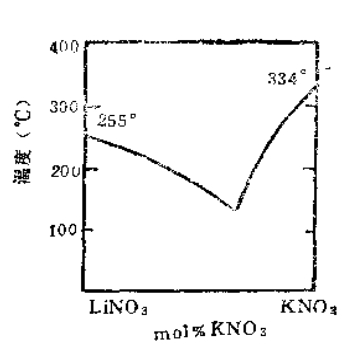
\includegraphics[width=0.5\textwidth]{fig/cp03/img3.1.jpg}
 \caption{$\rm LiNO_3-KNO_3$体系}
\end{figure}

\begin{figure}[thpb]
 \centering
 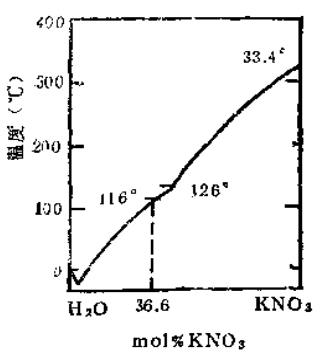
\includegraphics[width=0.5\textwidth]{fig/cp03/img3.2.jpg}
 \caption{$\rm H_2O-KNO_3$体系}
 (116℃是$\rm KNO_3$饱和溶液的沸点,126℃是$\rm KNO_3$的晶相转变温度)。
\end{figure}

如果从相图的观点来看问题,把溶液置于更广阔的范围内来讨论时,这些矛盾就可以统一起来了。例如在$\rm LiNO_3-KNO_3$体系的相图中(图3.1),低共熔点左右的两条液相线的范围是差不多的,都表示纯物质熔点因另一组分的加入而逐渐降低。该相图也可看成是溶解度图。此时,右边的曲线表示LiNO3在$\rm KNO_3$中的溶解度($\rm KNO_3$溶液);左边曲线则表示$\rm KNO_3$在LiNO3中的溶解度(LiNO3)。当状态点十分接近于$\rm KNO_3$熔点时(如成分为99.9\%的$\rm KNO_3$和0.1\%的LiNO3的样品在接近$\rm KNO_3$熔点(图3.1、图3.2)的温度下),LiNO3是液体,$\rm KNO_3$也在低于其熔点的温度下熔化。这种状态,一般认为是$\rm KNO_3$在少量LiNO3存在下熔化了,但也可以看成是999份$\rm KNO_3$溶解在1份LiNO3中。$\rm H_2O-KNO_3$体系的相图(图3.2)和$\rm LiNbO_3-KNO_3$体系是类似的。不同的是,其中一个组分,即H2O的熔点很低,左右两曲线的范围相差很大,但本质上没有什么差别。右边的曲线表示$\rm KNO_3$熔点因$\rm H_2O$的存在而下降的曲线,左边的曲线表示$\rm KNO_3$使$\rm H_2O$的冰点下降的曲线。由于$\rm H_2O$在常温下是液体,通常把右边曲线的下半部(图3.2中虚线左边,温度较低,含水量较多部分)看成$\rm KNO_3$在水中的溶解度曲线,而不是看成水使$\rm KNO_3$熔点降低的液相线。但在曲线的上部,我们虽然也可以把温度接近于$\rm KNO_3$熔点,含水量很少的液相(如含99.9\% $\rm KNO_3$,0.1\%$\rm H_2O$)看成是999份$\rm KNO_3$溶解在一份水中的溶液,但习惯上还是把这种情况看成$\rm KNO_3$在少量水的存在下熔化了。

由此可见,熔体和溶液是连续的,所以熔化和溶解在本质上是一样的。可以把熔化看成是被溶解所液化的特殊情况。当水是溶液的一个组分时,一般总是看成溶质(盐类)溶在一定温度的水中,而不是从水的存在使盐的熔点降低这个角度来看问题。习惯上把水多时称为溶解,而水很少时看成熔化。

 %溶液的概念
\subsection{溶解度和溶解度曲线}
溶解度是考察溶液中生长晶体的最基本参数。溶解度可用在一定条件(温度、压力)下饱和溶液的浓度来表示。溶质在溶液中的浓度(溶液成分)有以下几种表示方式:
\begin{enumerate}[(1)]\itemsep -0.5ex
\item 体积摩尔浓度(mol):一升溶液中所含溶质的摩尔数。
\item 重量摩尔浓度(mol):1000g溶剂中所含溶质的摩尔数。
\item 摩尔分数($x$):溶质摩尔数对溶液总摩尔数之比。
\item 重量百分数:100g(或是1000g)溶液中所含溶质的克数。
\item 重量比:100g(或是1000g)溶剂中所含溶质的克数。
\end{enumerate}

不同的浓度表示方式适用于不同的场合。在实验室中使用(1)表示方式是很方便的,但由于和溶液体积有关,易受温度影响(某一给定的摩尔随温度升高而减小),因此在溶解度数据中,经常使用其他浓度表示法,最常用的的是重量比和摩尔分数,后者特别适于多组分混合物的成分。

在数种质组成的溶液中,某一组分的摩尔分数可表示为
\begin{equation}
x_1=\frac{m_1/M_1}{m_1/M_1+m_2/M_2+m_3/M_3+\cdots},
\end{equation}
$m$是组分的重量,$M$是其分子量。任何混合物中所有成分的摩尔分数总和等于1。

各种浓度表示法可以互相换算,对于摩尔与其他浓度表示法换算时还需知道溶液的密度。在水溶液中,当溶质含有水合物和无水合物两种形式时,其重量百分数和重量比的换算公式如下:
\begin{equation}
c_1=\frac{100c_2}{100-c_2}=\frac{100c_3}{100R-c_3}=\frac{100c_4}{100R+c_4(R-1)},
\end{equation}
其中$c_1$为100g水中所含无水物的克数,$c_2$为100g溶液中所含无水物的克数,$c_3$为100g溶液中所含水合物的克数,$c_4$为100g水中所含水合物的克数;$R=\text{水合物分子量}/\text{无水合物分子量}$。

在我们所讨论的溶液体系中,压力对溶解度影响是很小的,但温度的影响却十分显著。这种温度-浓度关系可用溶解度曲线表示。图3.3示出一些常用水溶性晶体的溶解度曲线。从图3.3中可以看出,不同物质在水中的溶解度是有明显差别的。

%TODO: 图3.3
(图3.3)
% 图3.3一些水溶性晶体的溶解度曲线
%1.酒石酸钾钠(KNT); 2 .酒石酸钾(DKT); 3,酒石酸乙二胺(EDT);
%4.磷酸二氢铵(ADP);5.硫酸甘氨酸(TGS); 6.碘酸锂((L);7.磷酸二氢钾(KDP); 8.硫酸锂(LSH)。

有的晶体溶解度很大,如DKT,但有的则较小,如LSH,而大多数晶体的溶解度均随温度升高而增大(溶解度温度系数为正值)。有的晶体溶解度温度系数很大(如KNT),但也有少数晶体(如LSH,Li等),溶解度的温度系数很小,而且是负值。有的晶体溶解度曲线出现拐点(如EDT),这种物质有两种不同的溶解度晶相,即EDT无水物和水合物。图3.3中所示的溶解度曲线实际上是由EDT和$\rm EDT\cdot H_2O$两条溶解度曲线组成的,这两条曲线在拐点(40.6℃)相交。该点的温度称为相平衡转变温度。

溶解度曲线是选择从溶液中生长晶体的方法和生长温度区间的重要依据。如对于溶解度及其温度系数都很大的物质,采用降温法比较理想,而对于溶解度较大,而温度系数却较小的物质则宜采用蒸发法,对于具有不同晶相的物质则需选择对所需要的那种晶相是稳定的合适的生长温度区间。

温度对溶解度的影响可用下方程式表示:
\begin{equation}
\frac{d\ln{x}}{dT}=\frac{-\Delta H}{RT^2},
\end{equation}
式中$x$为溶质的摩尔分数,$\Delta H$为固体摩尔溶解热,$T$为绝对温度,$R$为气体常量。在理想情况下,式(3.3)可化为
\begin{equation}
\log x=\frac{-\Delta H}{2.303R}\left( \frac{1}{T}-\frac{1}{T_0}\right) =\frac{-\Delta H(T_0-T)}{4.579T_0T},
\end{equation}
$T_0$为晶体的熔点。从式(3.4)中可看出:
\begin{enumerate}[(1)]\itemsep -0.5ex
\item 大多数晶体的溶解过程是吸热过程,为正,温度升高,溶解度增大。如若是放热过程,则相反。
\item 在一定温度下,高熔点晶体的溶解度小于低熔点的溶解度。
\end{enumerate}

式(3.4)也可写成
\begin{equation}
\log x = -\frac{a}{T} + b,
\end{equation}
式中$a$和$b$都是常数。

温度对溶解度的影响也可表示为
\begin{equation}
c=A+Bt+Ct^2+\cdots,
\end{equation}
式中$c$为一定量溶剂中溶质的重量,$A,B,C$是和溶液体系(溶质-溶剂)有关的常数。式(3.5)和式(3.6)是表示温度对溶解度影响的最常用的表达式。

%TODO: 图3.4
(图3.4)

根据式(3.5)作图得出的溶解度曲线如图3.4(b)所示。图中的横坐标为溶质摩尔分数的对数坐标。右边纵坐标是(因为在273-373K范围内数值很小)的线性坐标。另外,也可以用专门的对数-倒数坐标图纸,将温度(℃)直接在图上标出。图3.4(b)中左边示出的纵坐标就是倒数标尺上直接标出的温度。将图3.4(a),(b)加以比较就可发现这种作图法有如下的一些优越性:
\begin{enumerate}[(1)]\itemsep -0.5ex
\item 线性好。在图3.4(a)中,在0-100℃范围内,CuSO4是平滑曲线,$\rm Na_2SO_4$和$\rm Na_2CrO_4$则分别是两条曲线在拐点(转变点)相交,而在图3.4(b)中,上述三种盐的溶解度曲线都是直线,但对一些溶解度很大的物质,或在很窄的温度区间内存在着数种水合物的物质,其溶解度仍是曲线。醋酸钠在40—50℃ 范围内直线发生弯曲,可能属于后一种情况。
\item 记录范围宽。对一些溶解度很大的盐类(如铬酸钠和醋酸钠的溶解度曲线)来说,都能像溶解度较小的盐类一样,在0-100 ℃范围内可出,这是通常的作图法无法做到的。
\item 较清楚地显示出转变点。例如通过两直线交点找$\rm Na_2SO_4$的转变点(32.4℃)要比图3.4(a)中所示延长两条曲线找转变点来得容易和准确。在图3.4(b)中,$\rm CuSO_4$的两条直线大约在67℃相交,表明硫酸铜在该处有不同的晶相转变,而在图3.4(a)中却找不出这一转变点。
\end{enumerate}

基于上述优点,利用$\log{x}-1/T$图可以用内插法和外推法求出溶解度的数值,并估计出转变温度(如果存在相平衡转变)。因此,式(3.5)在实践中很有用。 %溶解度和溶解度曲线
\subsection{饱和与过饱和}
与溶质固相处于平衡状态的溶液称该物质的饱和溶液。溶解度曲线实际上给出不同温度下的饱和溶液的浓度,所以溶解度曲线也称为饱和曲线。在一定条件下,对给定的物质,这条曲线是确定的,可以通过准确测定物质在不同温度下的溶解度绘制出来。

(图3.5)

如果A为溶质,B为溶剂,A与B之间也不形成任何化合物,

(图3.6)

则图3.6中的溶解度曲线就是图3.5中液相线的一部分$\alpha\beta$。图3.6中曲线$\alpha\beta$的下部是不饱和溶液区,$\alpha\beta$的上方是固相和溶液共存区。当溶液状态进入该区时,应当结晶出固相A,此时的溶液浓度应为在该温度下和固相A相平衡的饱和溶液的浓度。但实际上,这样的溶液常常不析出晶体。这种所含溶质量比在同一条件下饱和溶液中所含溶质量要多的溶液称为过饱和溶液。凡是状态点处在饱和曲线以上区域内的溶液都是过饱和溶液,所以这个区域也称为过饱和溶液区。

溶液都具有程度不同的过饱和现象。过饱和状态是从溶液中生长晶体的前提条件,因此从上一世纪以来就对过饱和溶液进行了较深人的研究。

过饱和状态在热力学上是不稳定的,整个过饱和区的不稳定程度也是不一样的。溶液状态靠近饱和曲线就较为稳定,离饱和曲线越远就越不稳定。1897年Ostwald首先引入“不稳过饱和” 和“亚稳过饱和”的概念。他把在无晶核存在的情况下能自发析出固相的过饱和溶液称为“不稳过饱和”溶液,而把不能自发结晶的过饱和溶液称为“亚稳过饱和”溶液。

随后,Miers对自发结晶和过饱和度之间的关系进行了广泛的研究。他测量了许多盐类的浓溶液在冷却过程中折射率的变化,试图找出过饱和溶液中不稳区和亚稳区的界限。他的实验结果可用图3.7来表示,图中除了溶解度曲线外,在其上方还有一条溶液开始自发结晶的界限,称为过溶解度曲线.这条曲线将过饱和溶液分为亚稳区和不稳区。过溶解度曲线不像溶解度曲线那样确定,极易受一些外界因素(如溶液搅拌程度)影响。关于这一观点引起了很大争论,有的人认为不可能存在这样一条使溶液性质突然起变化的曲线,有的人则倾向于把过溶解度曲线看成是位于过饱和区的一个区域或窄带。

(图3.7)

但是不论过溶度曲线是否真实存在,但在过饱和区,靠近溶解度曲线确实存在亚稳区,这个事实是毋庸置疑的。整个温度-浓度图还是可分成稳定区、亚稳区和不稳区三个区域,其中稳定区是确定的,而亚稳区和不稳区在一定程度上是可变的,很难严格区分。这些区域的特征如下:

稳定区:即不饱和区,不可能发生结晶作用。

亚稳(过饱和)区:处于这个区域的溶液不会自发地发生结晶作用。如将籽晶放人处于亚稳区的溶液中,晶体就会在籽晶上生长。

不稳(过饱和)区:处于这个区域的溶液会自发地发生结晶作用。

三个区域以亚稳区最为重要,因为从溶液中生长晶体都是在这个区域内进行的。从培养单晶的角度出发,我们总希望析出的溶质都在籽晶上逐渐生长而不希望中出现自发晶体(即杂晶),为此要求在整个生长过程中使溶液状态始终保持在亚稳区内。亚稳区虽无法精确测量, 但其大小、趋向还是可以用过饱和度(或过冷度)来估计的。亚稳区的大小既同结晶物质的本性有关,也极易受外界条件的影响, 如搅拌、振动、温度、杂质等。不同物质溶液的亚稳区差别相当大(见表3.2)。过饱和度有以下几种表示方式:
\begin{eqnarray}
&& \text{浓度驱动力}\ \Delta c,\quad\Delta c=c-c^*; \\
&& \text{过饱和比}\ s,\quad s=\frac{c}{c^*}; \\
&& \text{过饱和度或相对过饱和度}\ \sigma,\quad\sigma=\frac{\Delta c}{c^*}=s-1,
\end{eqnarray}
其中$c$是溶液的实际浓度,$c^*$是溶液在同一温度下的平衡饱和浓度(图3.7)。在以上三种表示方式中,只有是有量纲的(用摩尔分数表示是例外),其数值随浓度表示方式的不同而差别很大,但对$s$和$\sigma$的影响却不很明显(表3.1)。表示过饱和度时,必须注明溶液温度,因为溶液的平衡饱和浓度是随温度的变化而变化。

%TODO: 表3.1 3.2
(表3.1)(表3.2)

过饱和度也可用温度来表示。若将某一物质在$t^*$℃时,将其饱和溶液冷却至$t$℃,溶液进入过饱和状态,如果没有结晶析出,则该溶液的过饱和度为$\Delta t=(t^*-t)$(见图3.7),这实际上就是溶液的过冷度(在单组分体系中,只用过冷度而不使用过饱和度这个名词)。一些盐类水溶液的最大可容许过冷度列于表3.2中。这些数据是将25℃的饱和溶液在有晶体存在和适当搅拌的情况下,通过缓慢降温测得的。虽然在实验室条件下测得的过冷度和生产实践中的情况有较大差别,但也可以作为对在该实验条件下比较不同物质溶液亚稳区大小的量度。过冷度和过饱和度的关系为
\begin{equation}
\Delta c = \left(\frac{dc^*}{dt}\right)\Delta t.
\end{equation}
 %饱和与过饱和
\subsection{溶液饱和温度、溶解度和过饱和度的测定}
溶液到达饱和状态时的温度,即溶质固体和溶液达成平衡的温度称为溶液的饱和温度。准确地测定溶液的饱和温度是搞好下种操作的前提,也是测定溶解度和过饱和度的基础,所以饱和温度的测定是从溶液中培养晶体的一项基本功。常用的测定饱和温度的方法有以下几种:

\paragraph{(1) 平衡法}
在接近饱和的溶液中,放人一些溶质固体,在一定温度下不断搅拌,直到溶液中尚余少量固体不再溶解为止,此时溶液的温度即可看成是溶液的饱和温度。这个方法虽然简便,但要达到真正平衡所需的要达到真正平衡所需的时间较长(约数小时至数天,视溶液的粘度和搅拌强度而定),而且精确度也较低,约0.5—1℃。

\paragraph{(2) 浓度涡流法}
(图3.8)
%TODO:Fig.3.8
用尼龙线将一小块晶体悬在其接近饱和温度的溶液中,仔细观察晶体及其附近的液流情况。如果溶液是不饱和的,则晶体稜角变得圆滑。靠近晶体表面的溶液,由于晶体的溶解,其浓度比周围溶液浓度大,因而变得较重而向下运动,形成一股向下的液流, 并把这股液流称为溶解涡流。如果溶液是过饱和的,则晶体呈现生长 现象,晶面变光滑,稜角“发毛”变白。晶体附近的溶液由于溶质在晶体上析出,密度变小,因而形成一股向上运动的液流,称为生长涡流(图3.8)。涡流是溶液中浓差造成的对流运动。距饱和温度越远,涡流越明显;离饱和温度愈近,涡流就愈微弱;在饱和温度下,涡流完全消失。因此,可以通过观察涡流的变化来确定饱和温度。在测定时,可从不饱和状态开始,逐渐降低温度,观察晶体附近的浓差涡流从溶解涡流减弱到生长涡流出现的过程,找出涡流消失时的温度,即为溶液的饱和温度。为了提高准确度,可反复数次通过饱和点进行测定。这个方法的精确度约为0.1—0.5 ℃(与观察者熟练程有关)。使用该法时,要防止溶液分层,测定前溶液应充分搅拌,测定时只让溶液发生自然对流。

\paragraph{(3) 光学效应法}
溶液接近饱和温度时,涡流十分微弱,凭肉眼要把温度测定得很精确是困难的,光学效应法可以克服这一缺点。

当晶体处于与它不相平衡的母液中时,紧贴晶体附近有一薄层溶液,晶体溶解和生长时,溶质的扩散输出和输入都通过这一薄层进行,该薄层溶液称为扩散层或结晶区。扩散层存在浓度梯度,当溶液接近饱和温度时,扩散层的浓度梯度趋于消失。溶液到达饱和温度时,扩散层消失。扩散层是浓度不均匀的区域,因此在光学上也是不均匀的,光线通过这一区域时会因折射率梯度方向不同而发生不同的偏折,光学效应法的原理就基于此。常用的光学效应法有下两种类型。

\subparagraph{(i) 纹影法}
(图3.9)
%TODO:Fig.3.9
其装置如图3.9所示。这种装置适用于观察透明介质中的局部光学不均匀性。光源$S$通过$O_1$,聚焦至可调孔径光栏$R_1$即$O_2$的焦点上,光线透过$O_2$即变成平行光照射到待测的不均匀透明介质上,经$O_3$成像于焦点$S'$,在该处放置一锐边遮光板或狭缝$R_2$,挡住了光源的像$S'$,因此在白色的屏幕上出现黑色的背景,但在$SS'$之间存在光学不均匀区域$A$,则光线发生偏折,从$R_2$的锐边旁通过在屏幕上给出其像$A'$。偏折方向与不均匀区域的折射率梯度方向有关。这种方法能发现折射率差别很小的不均匀区域。在光路中的待测生长池$K$中,晶体附近的不均匀扩散层可以在屏幕上清楚地显示出来。在不饱和的溶液中,扩散层的像出现在无遮光板一侧的晶体附近,在过饱和溶液中则恰好相反,如图3.9所示。当溶液到达饱和状态时,扩散层消失。在测定时,溶液可以不停地搅拌,生长池的温度可用电热吹风机调整。这种方法的精确度可达0.05℃,甚至更高。值得注意的是,光源应用单色光,用He-Ne激光更好,否则,$O_2,O_3$应用消色差透镜。

\subparagraph{(ii) 狭缝光源法}
该法是使一狭缝光源和置于待测溶液中晶体的一个晶面斜交,随着溶液状态的变化,在狭缝和晶面的交界处会出现不同的偏折现象,这也是由于存在扩散层这一光学上不均匀的区域所引起的。

(图3.10)
%TODO:Fig.3.10

当溶液不饱和时,明亮的狭缝在晶面交界处弯曲成钝角,当溶液为过饱和时,则向相反方弯曲成锐角。溶液愈偏离饱和状态,弯曲现象就越明显。随着溶液逐淅接近饱和,弯曲部分逐渐缩短,当溶液达到饱和时,狭缝光在晶面交界处不发生弯曲(图3.10)。根据这种现象所测定的饱和温度的精确度也可达到0.05℃。 使用这一方法时,可将盛有待测溶液的容器放在恒温槽中进行测量,也可通过特定装置将溶液从大育器中抽出,流过调温装置和测量装置,再泵浦回育晶器,这样可以迅速而准确地测定育晶器中溶液的饱和温度,在生产和实验室中使用这种方法是很方便的。

利用上述测定饱和温度的方法,特别是光学效应法,也可以进行溶解度的测定,并绘制出溶解度曲线。溶解度测定虽较简单,但需要有高度的实验技巧和精确度。

用平衡法测溶解度时,在到达平衡后应恒温静置使细小分散的固体颗粒沉降,仔细抽取一定量(不是一定体积)的溶液样品进行分析,确定溶液成分。溶液分析通常用重量法和容量法,有时也使用其他方法(如比色法以及密度、折射率、电导等方法)。溶液成分也可以预先准确配制(即称取一定量的溶剂和溶质),然后再测出溶液的饱和温度,确定其溶解度。

在确定溶液成分的同时,也有必要对与之相平衡的固相进行分析鉴定。有时在很小的温度区间内与饱和溶液相平衡的稳定相是可以改变的,转别是水合物体系。例如在0-100 ℃区间内测定$\rm Na_2CO_3$在水中的溶解度时发现,在32℃以下,其稳定相是$\rm Na_2CO_3\cdot 10H_2O$,而$\rm Na_2CO_3\cdot 7H_2O$在32.0℃到35.4℃之间稳定,$\rm Na_2CO_3\cdot H_2O$在35.4℃以上稳定。因此,必须将不同温度下的平衡固相晶体取出,在该温度下仔细于燥,并确定其成分。对于成分相同但结构不一样的不同晶相(多形体),还必须利用物理鉴定的方法来确定与溶液相平衡的物相。例如从高浓度重水($\rm D/(D+H)=99.8\%$)溶液中,生长磷酸二氘钾(DKDP)晶体时,DKDP会出现四方和单斜两种晶相。在21℃以下时,四方相是与溶液平衡的稳定相,在21℃以上时,单斜相是稳定相。这两相的溶解度十分接近(特别是在转变点附近),因此用通常测定溶解度的方法很难将它们区分开来。在这种情况下,光学效应法就显示出其优越性。图3.11示出的四方和单斜两相溶解度曲线就是用图3.9的装置测定出来的。对每一相不仅测定了在其相稳定区内(即稳定相)的溶解度曲线,还成功地测出了在另一相稳定区内(即亚稳相,参阅3.2.3节)的溶解度曲线,这样对四方相和单斜相都测出了一条完整的溶解度曲线。这两条曲线的交点即为DKDP溶解度曲线上的拐点,即四方相和单斜相的相平衡转变点(在图3.11中转变点为21 ℃)。

(图3.11)
%TODO:Fig.3.11
必须指出的是,在测定溶解度曲线的工作中,提高控温和测温的精度是十分重要的。例如在测定氯化钠在30℃水中的溶解度时,实验温度波动±0.5℃,引起溶解度测量误差约0.1\%,但在测定硫酸钠在30℃水中的溶解度时,同样的温度波动则能造成5\%的误差。所以在测定工作中,恒温器所用的温度计必须用标准温度计进行校正。

过饱和度是影响晶体生长速度和质量的重要因素,过饱和度的确定对晶体生长研究工作和培养单晶的实践都有重要意义。如果在给定温度下,溶液的浓度可以测量出来,而且相应的平衡饱和浓度是已知的,那么就不难根据式(3.7)-(3.9)来计算溶液的过饱和度。上述已提到,溶液浓度可以进行直接的分析,也可通过测量体系中某些对浓度变化敏感的性质(如密度、粘度、折射率和电导率等)来间接确定。在实验室的条件下,这些性质都可以测量得很精确。但在晶体培养过程中,要求在不破坏液体稳定性的条件下,能在育晶器中进行连续的测量。如果在生长过程中温度是变化的,还需知道被测量性质对温度的依赖关系,这样,问题就变得复杂了,因此直接应用还是较少。在上述对浓度敏感的性质中,密度和折射率对温度较不敏感。

溶液的过饱和度也可以用光学效应法在生长过程中直接测定,所得的过饱和度是以过冷度$\Delta t$表示的。这种方法的优点就是不需要知道溶液的准确成分和溶解度曲线,也不需改变育晶器的温度,在晶体生长过程中,任何时候都可测得溶液的真实过饱和度。遗憾的是,在晶体的生长过程中,抽取溶液进行循环流动,有破坏溶液稳定性,影响晶体生长的危险。但在三槽流动法中,对过热槽中的饱和度用上述方法进行测量则是十分安全和方便的。

各种过饱和度的测量方法,虽取得了一定的效果,但都存在着不少问题,有待于进一步研究解决,并希望能创造更简便、灵敏、可靠的能连续进行测量的新方法。 %溶液饱和温度、溶解度和过饱和度的测定
\subsection{溶剂的选择和水溶液的结构}
 %溶剂的选择和水溶液的结构
\setcounter{section}{1}
\section{溶液中晶体生长的平衡}

\subsection{平衡和结晶过程的驱动力}
晶体生长是一个不平衡的过程。晶体在平衡状态时既不溶解也不生长,但要研究晶体生长过程,必须掌握有关该过程中平衡状态的知识。

溶液中生长晶体最重要的参数(平衡特征)是溶解度。溶解度曲线给出溶液的饱和浓度,即与固相处于平衡状态的溶液浓度。

可以把晶体生长看成是多相化学反应。当固体物质A在溶剂中溶解并达到饱和时,可用下述化学平衡方程式描述
\begin{equation}
\mathrm{A_{\text{固}} \rightleftharpoons A_{\text{溶解}}}
\end{equation}
\begin{equation}
K=\frac{[a]_e}{[a]_e(s)}
\end{equation}
其中$[a]_e$为饱和溶液中的平衡活度;$[a]_e(s)$为固相中的平衡活度,$K$为平衡常数。通常选取标准状态,使固体物质的活度等于1,此时,浓度单位最好用摩尔分数,这样上述方程就可在多组分的体系中应用。

组分活度$a_i$与其摩尔分数$x_i$的关系为
\begin{equation}
a_i = \gamma_i x_i
\end{equation}
$\gamma_i$是某组分$i$的活度系数,若$\gamma_i=1$,则该组分服从Raoult定律。如其活度系数不等于1,但仍是常数,则该组分服从Henry定律\footnote{Raoult定律:{$p=p_0x$}。{$p$}为溶液蒸汽压,$p_0$为纯溶剂蒸汽压,$x$为物质摩尔分数;Henry定律:$p=kx$,$p$为物质在溶液上的蒸汽压,$x$为物质摩尔分数,$k$为常数。}。

在理想溶液中,溶剂和溶质都服从Raoult定律,溶液的焓和体积分别等于溶剂和溶质的焓和体积之和。这意味着在溶解时,混合热和体积变化都等于零,但溶液的熵并不等于其组分熵的总和,因为熵是随无序性增加而增加的。在非理想的稀溶液中,溶质服从Henry定律,而溶剂则服从Raoult定律。

在3.1.1节中已提到,通常把溶液中含量较大的、即摩尔分数接近1的组分看作溶剂。浓溶液(溶剂和溶质含量差不多)并不服从Raoult定律和Henry定律,活度系数和浓度有关,需根据实验数据来估计。生长晶体的溶液大多是浓溶液,因此要考虑溶质质点间的相互作用,并在此基础上进行一些计算。

溶解度与温度的依赖关系可用Van't Hoff方程表示
\begin{equation}
\frac{\mathrm{d}\ln k}{\mathrm{d}T} = \frac{-\Delta H}{RT^2}.
\end{equation}
对溶液,上式变为
\begin{equation}
\frac{\mathrm{d}\ln [a]_e}{\mathrm{d}T} = -\frac{\overline{\Delta H}}{RT^2}.
\end{equation}
$\overline{\Delta H}$为溶质A在溶剂B中的偏摩尔焓的变化量,即表示将1摩尔溶质转移到体积足够大的溶液中时(此时溶液浓度不明显偏离饱和浓度)焓的变化、即溶解热(见3.1.6节)。在服从Raoult定律的溶液中,可用$x_A$来代替组分A的活度。

在溶液里生长晶体的过程中,自由能的变化为
\begin{equation}
\Delta G=\Delta G^0+RT\ln Q,
\end{equation}
其中
$$\Delta G^0=-RT\ln k,$$
$$Q=[a]^{-1},$$
$\Delta G^0$是生长过程中自由能的变化,$k$是式(3.19)的倒数,$[a]$是组分A在过饱和溶液中的实际活度。代入式(2.23)可得
\begin{equation}
\Delta G=RT\ln\frac{[a]_e}{[a]}
\end{equation}
其中$[a]_e$是组分A在饱和溶液中的平衡活度。若活度系数$\gamma=1$或是在一定范围内,$\gamma$和浓度无关,则在式(3.22)和式(3.24)中活度可用摩尔分数或浓度代替。因此式(3.24)中的$[a]_e/[a]$可用$c^*/c$代替。$c$和$c^*$分别是溶液在一定温度下的实际浓度和饱和浓度。根据式(3.8),$c/c^*$又是衡量过饱和度大小的过饱和比$s$,所以
\begin{equation}
\Delta G=RT\ln c^*/c = -RT\ln s
\end{equation}
从式(3.25)中可以看出,在过饱和溶液中($s>1$),生长晶体的过程是自由能降低的过程。这一过程是自动进行的。过饱和是结晶过程的驱动力。$s$愈大,自由能降低也愈多。晶体生长的驱动力也愈大。
 %平衡和结晶过程的驱动力
\subsection{分配系数}
溶液生长中平衡的一个重要方面是除溶质和溶剂外的第三个组分(包括杂质、掺质和同位素置换等)在固相中的溶解度问题,也就是该组分在固相和与之相平衡的液相之间的分配问题。

如果第三个组分(以下简称物质)在溶液和固相之间达成平衡时,有
\begin{equation}
\text{物质在液态溶液中的活度}(a_l) \rightleftharpoons \text{物质在固态溶液中的活度}(a_s),
\end{equation}
则
\begin{equation}
k_0=a_s(e)/a_l(e),
\end{equation}
$k_0$称为平衡分配系数。对于接近理想溶液的稀溶液来说,有
\begin{equation}
k_0=c_s(e)/c_l(e),
\end{equation}
$c_s(e)$和$c_l(e)$分别是物质在固相和溶液中的平衡浓度,即在液相和固相分界处的浓度。显然,要达到平衡时的分配系数,就要求晶体在溶液中既不溶解也不生长,或是生长速度很慢以至接近于平衡状态。另外,物质在两相中的浓度也不宜太大,以便用浓度来代替活度。

晶体在溶液中生长时,靠近晶体表面存在着扩散层(结晶区)。物质在扩散层中的浓度和在整个溶液中的浓度是有差别的。这一差别的程度取决于分配系数$k_0$的大小以及晶体生长的速度(对于给定物质,主要取决于后者)。在使用式(3.28)时,$c_l(e)$应该是物质在扩散层中的浓度,实际上这一浓度是无法测量的,因此引入有效分配系数$k_\text{eff}$的概念,定义如下
\begin{equation} k_\text{eff} = \frac{c_s}{c_l}, \end{equation}
$c_s$和$c_l$分别是物质在固相和溶液中(远离生长界面)的实际浓度。显然,$k_\text{eff}$和晶体生长速度有关,而后者又取决于过饱和度和扩散层的厚度。当溶液中的浓度接近等于晶体界面附近溶液浓度时,即$c_l \approx c_l(e)$,则$k_\text{eff} \approx k_e$(因为在大多数情况下,$c_s \approx c_s(e)$)。

当单晶在溶液中生长时,由于晶体的各向异性,$k_\text{eff}$也和结晶方向有关。例如Fe$^{3+}$在KDP晶体的柱面和锥面上的分配系数并不一样,这样就给确定$c_s$和分配系数带来很多的困难。

总之,有效分配系数和晶体生长速度溶液的搅拌情况(影响扩散层厚度)以及结晶方向都有关系,如果测得的分配系数和上述几方面都关系不大时,我们就可认为体系接近于平衡状态,即$k_\text{eff} = k_e$。

有效分配系数还和物质的浓度有关。例如在重水溶液中生长DKDP晶体时,氘在晶体中的浓度$x$(以摩尔分数表示,$x=D/(D+H)$),取决于氘在溶液中的浓度(以摩尔分数$y$表示),其有效分配系数($k_\text{eff}(D) = x/y$)和$y$有关,关系式为
\begin{equation}
k_\text{eff}(D) = 0.68\exp(0.382y),
\end{equation}
D和H在溶液和晶体中的分布是均匀的,在氘化程度较高的溶液中,也可将D$_2$O看成溶剂,而把H$_2$O看成第三个组分(杂质)来计算氢的有效分配系数$k_\text{eff}(H)$
\begin{equation}
k_\text{eff}(H)=(1-x)/(1-y).
\end{equation} %分配系数
\subsection{相稳定区和亚稳相生长}
许多物质在水溶液中可以形成数种不同的晶相。例如硫酸钠在水溶液中形成$\rm Na_2SO_4$和$\rm Na_2SO_4\cdot 10H_2O$两种固相(图3.14)。

\begin{figure}[h]
 \centering
 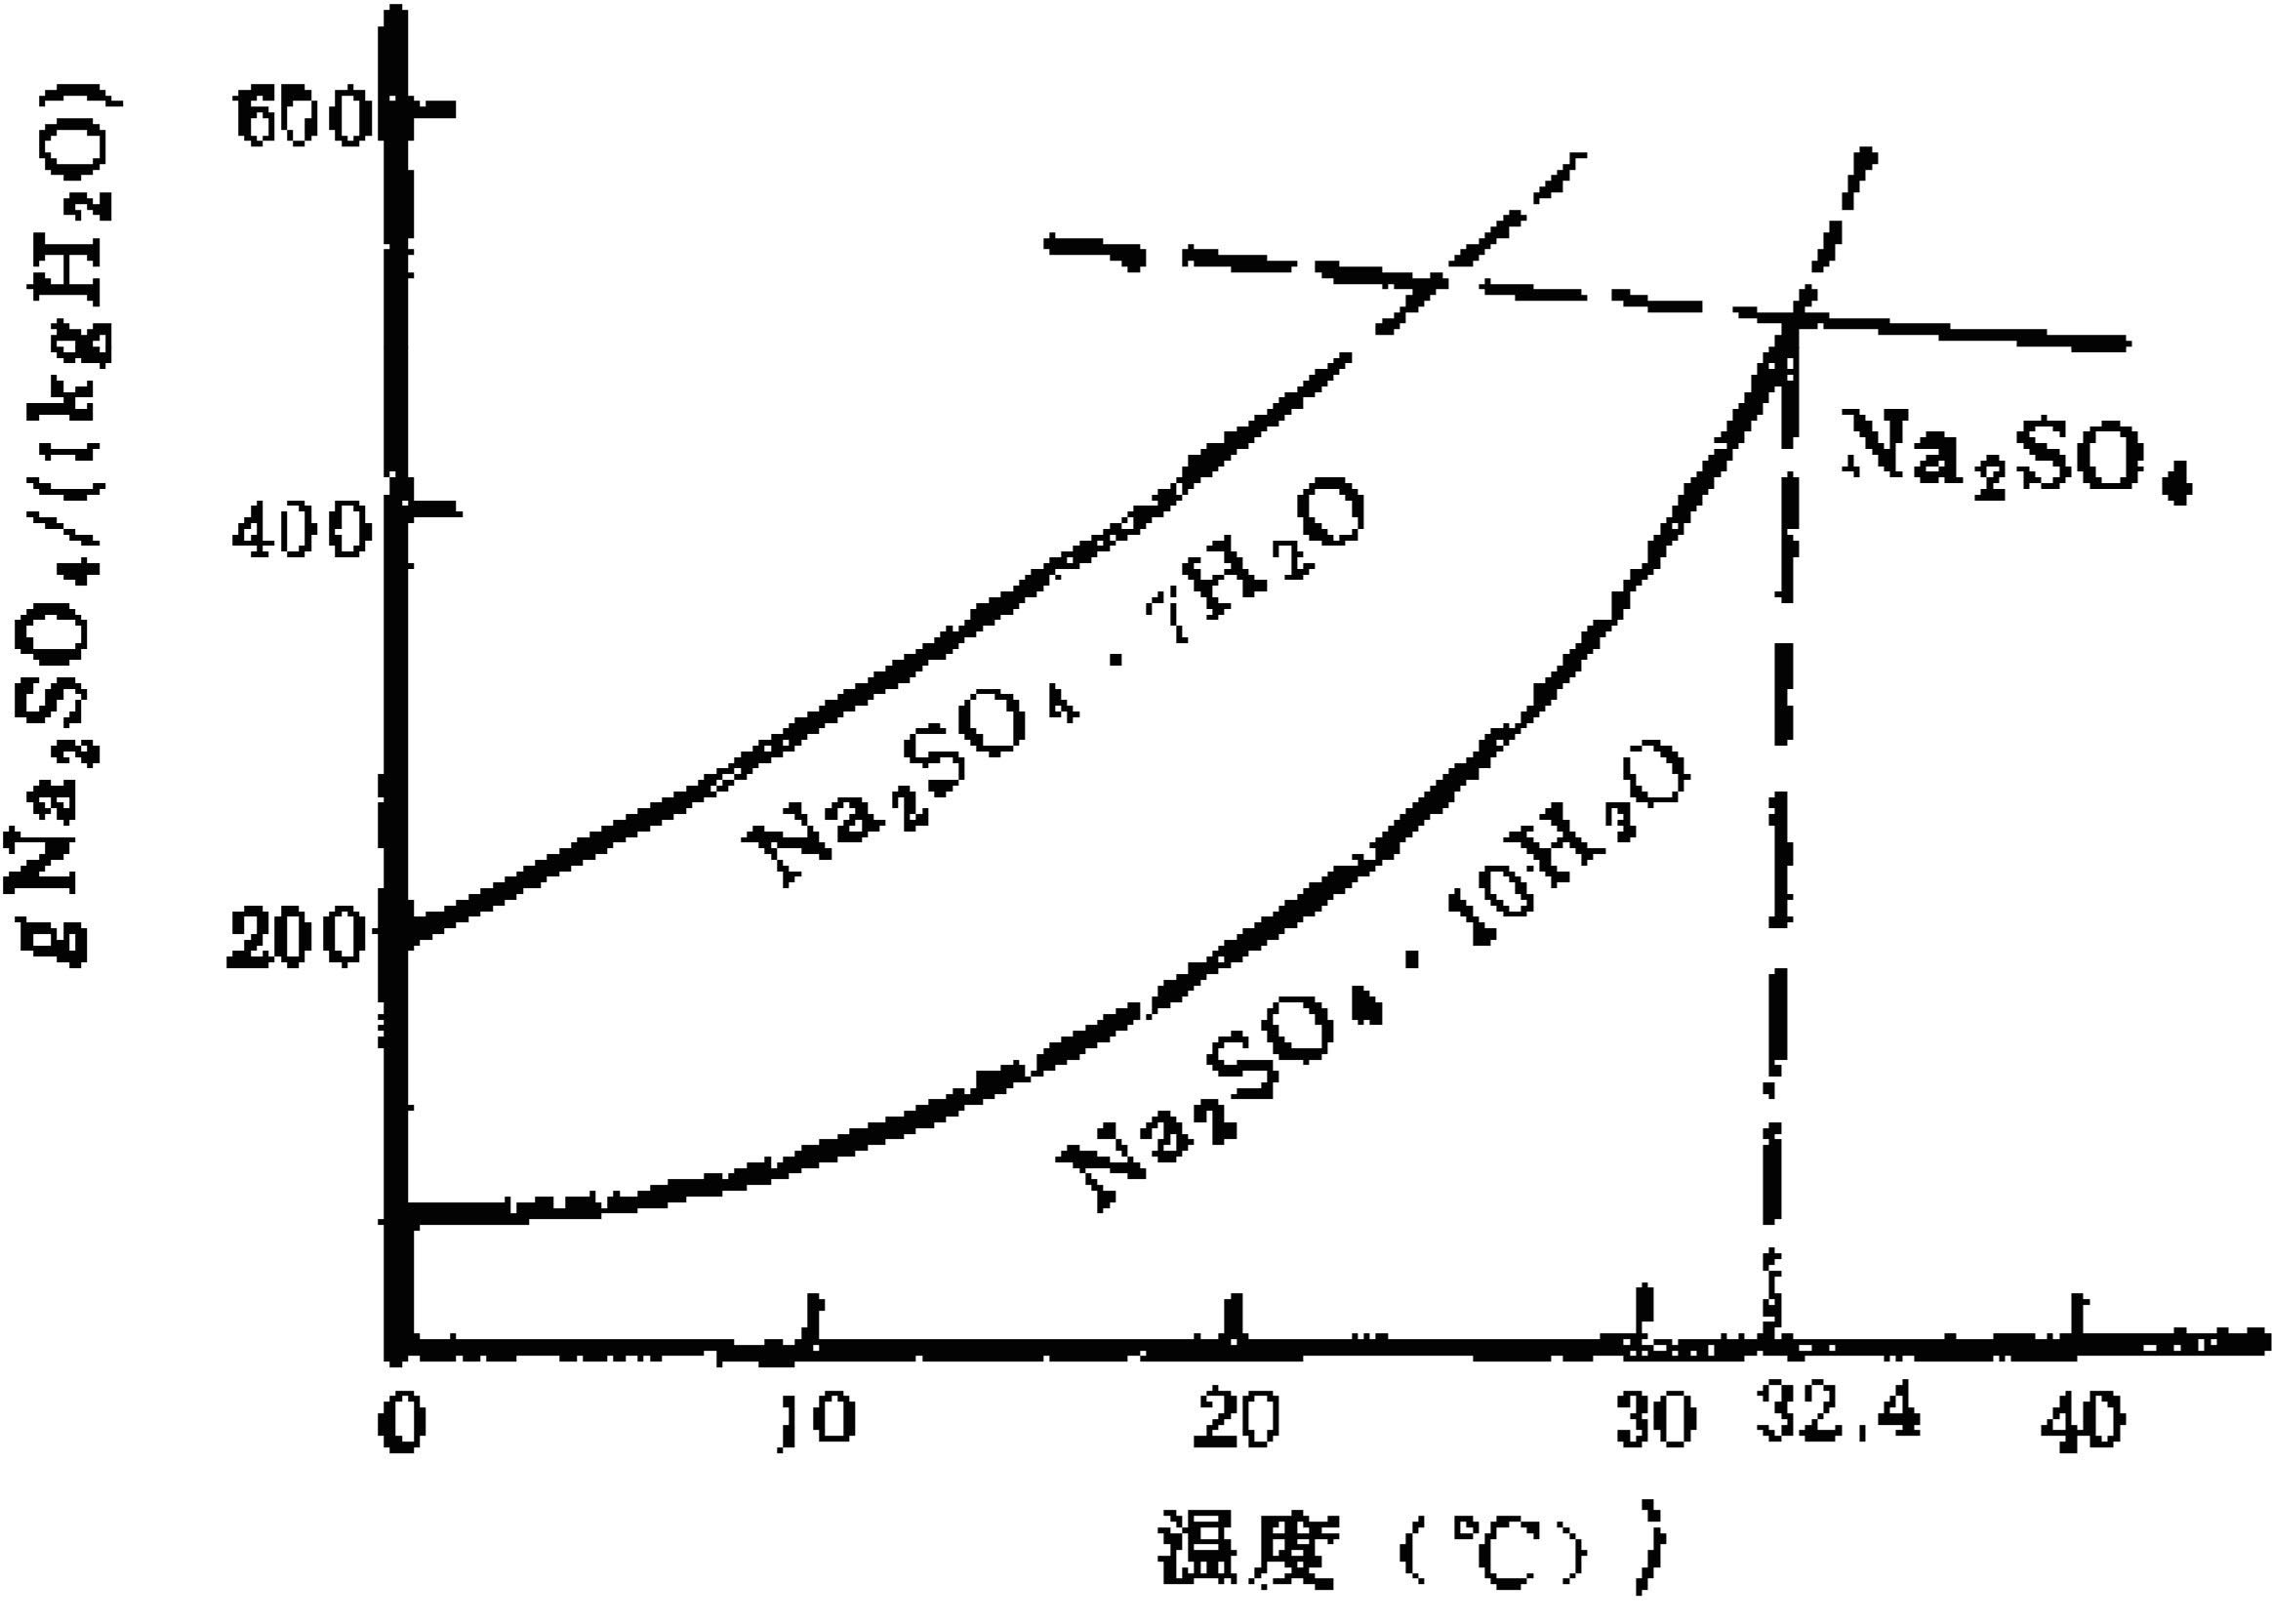
\includegraphics[width=0.8\textwidth]{fig/cp03/img3.14.jpg}
 \caption{$\rm Na_2SO_4-H_2O$体系。}
\end{figure}

\begin{figure}[h]
 \centering
 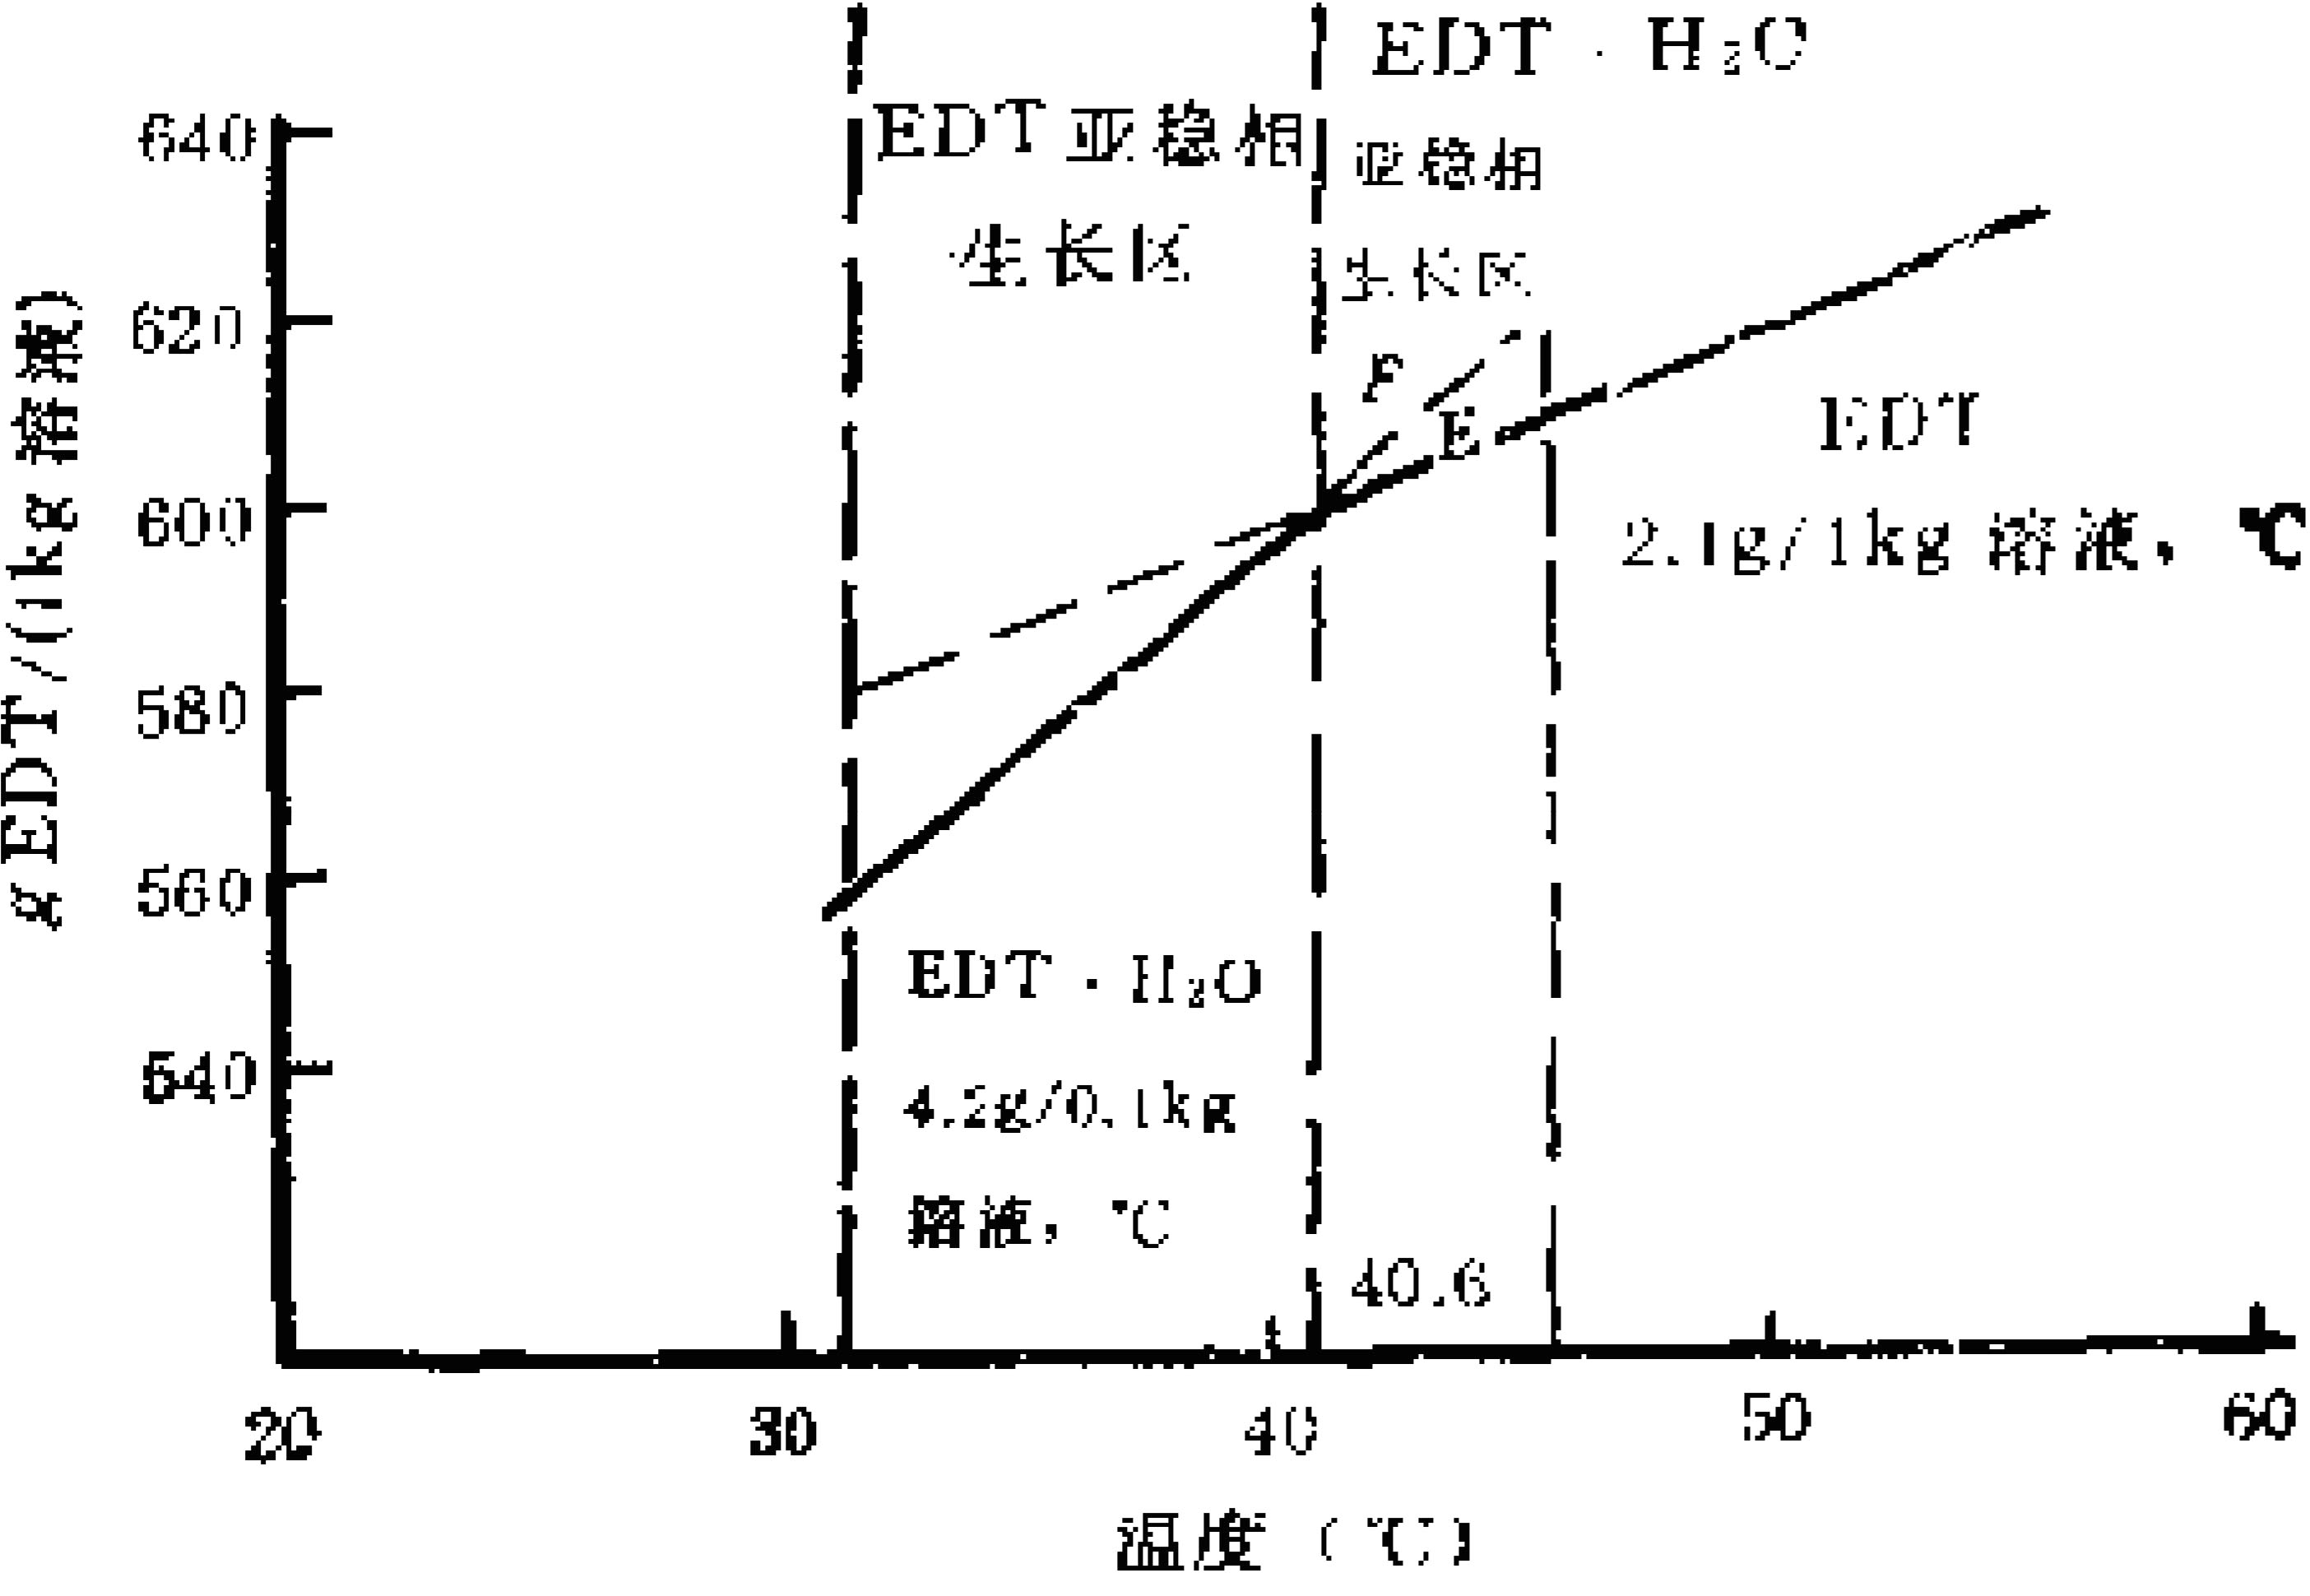
\includegraphics[width=0.8\textwidth]{fig/cp03/img3.15.jpg}
 \caption{$\rm EDT-H_2O$体系。}
\end{figure}

EDT在水溶液中,有EDT和$\rm EDT\cdot H_2O$两种结晶(图3.15)。这两个体系都是二组分体系,根据相律,在三相共存时只有一个自由度。如果压力固定(1atm),则体系是不变的。这就是说,两种晶相同时与溶液达成平衡的温度(即相平衡转变温度,以下简称转变温度)是完全确定的。硫酸钠的转变温度为32.4℃,EDT的转变温度为40.6℃。DKDP(通常为$\rm KD_{2x}H_{2(1-x)}PO_4$)在重水溶液中会出现四方和单斜两种结晶相,该体系可看成是$\rm DKDP-D_2O/D_2O+H_2O$准二组分体系,在三相达成平衡时,若压力固定(1atm),则两固相与溶液达成平衡的转变温度随$\rm DKDP-D_2O/D_2O+H_2O$的变化而变化。(图3.16)。对于D2O含量为99.8\%的溶液,DKDP的转变温度为21℃(见图3.11)

\begin{figure}[h]
 \centering
 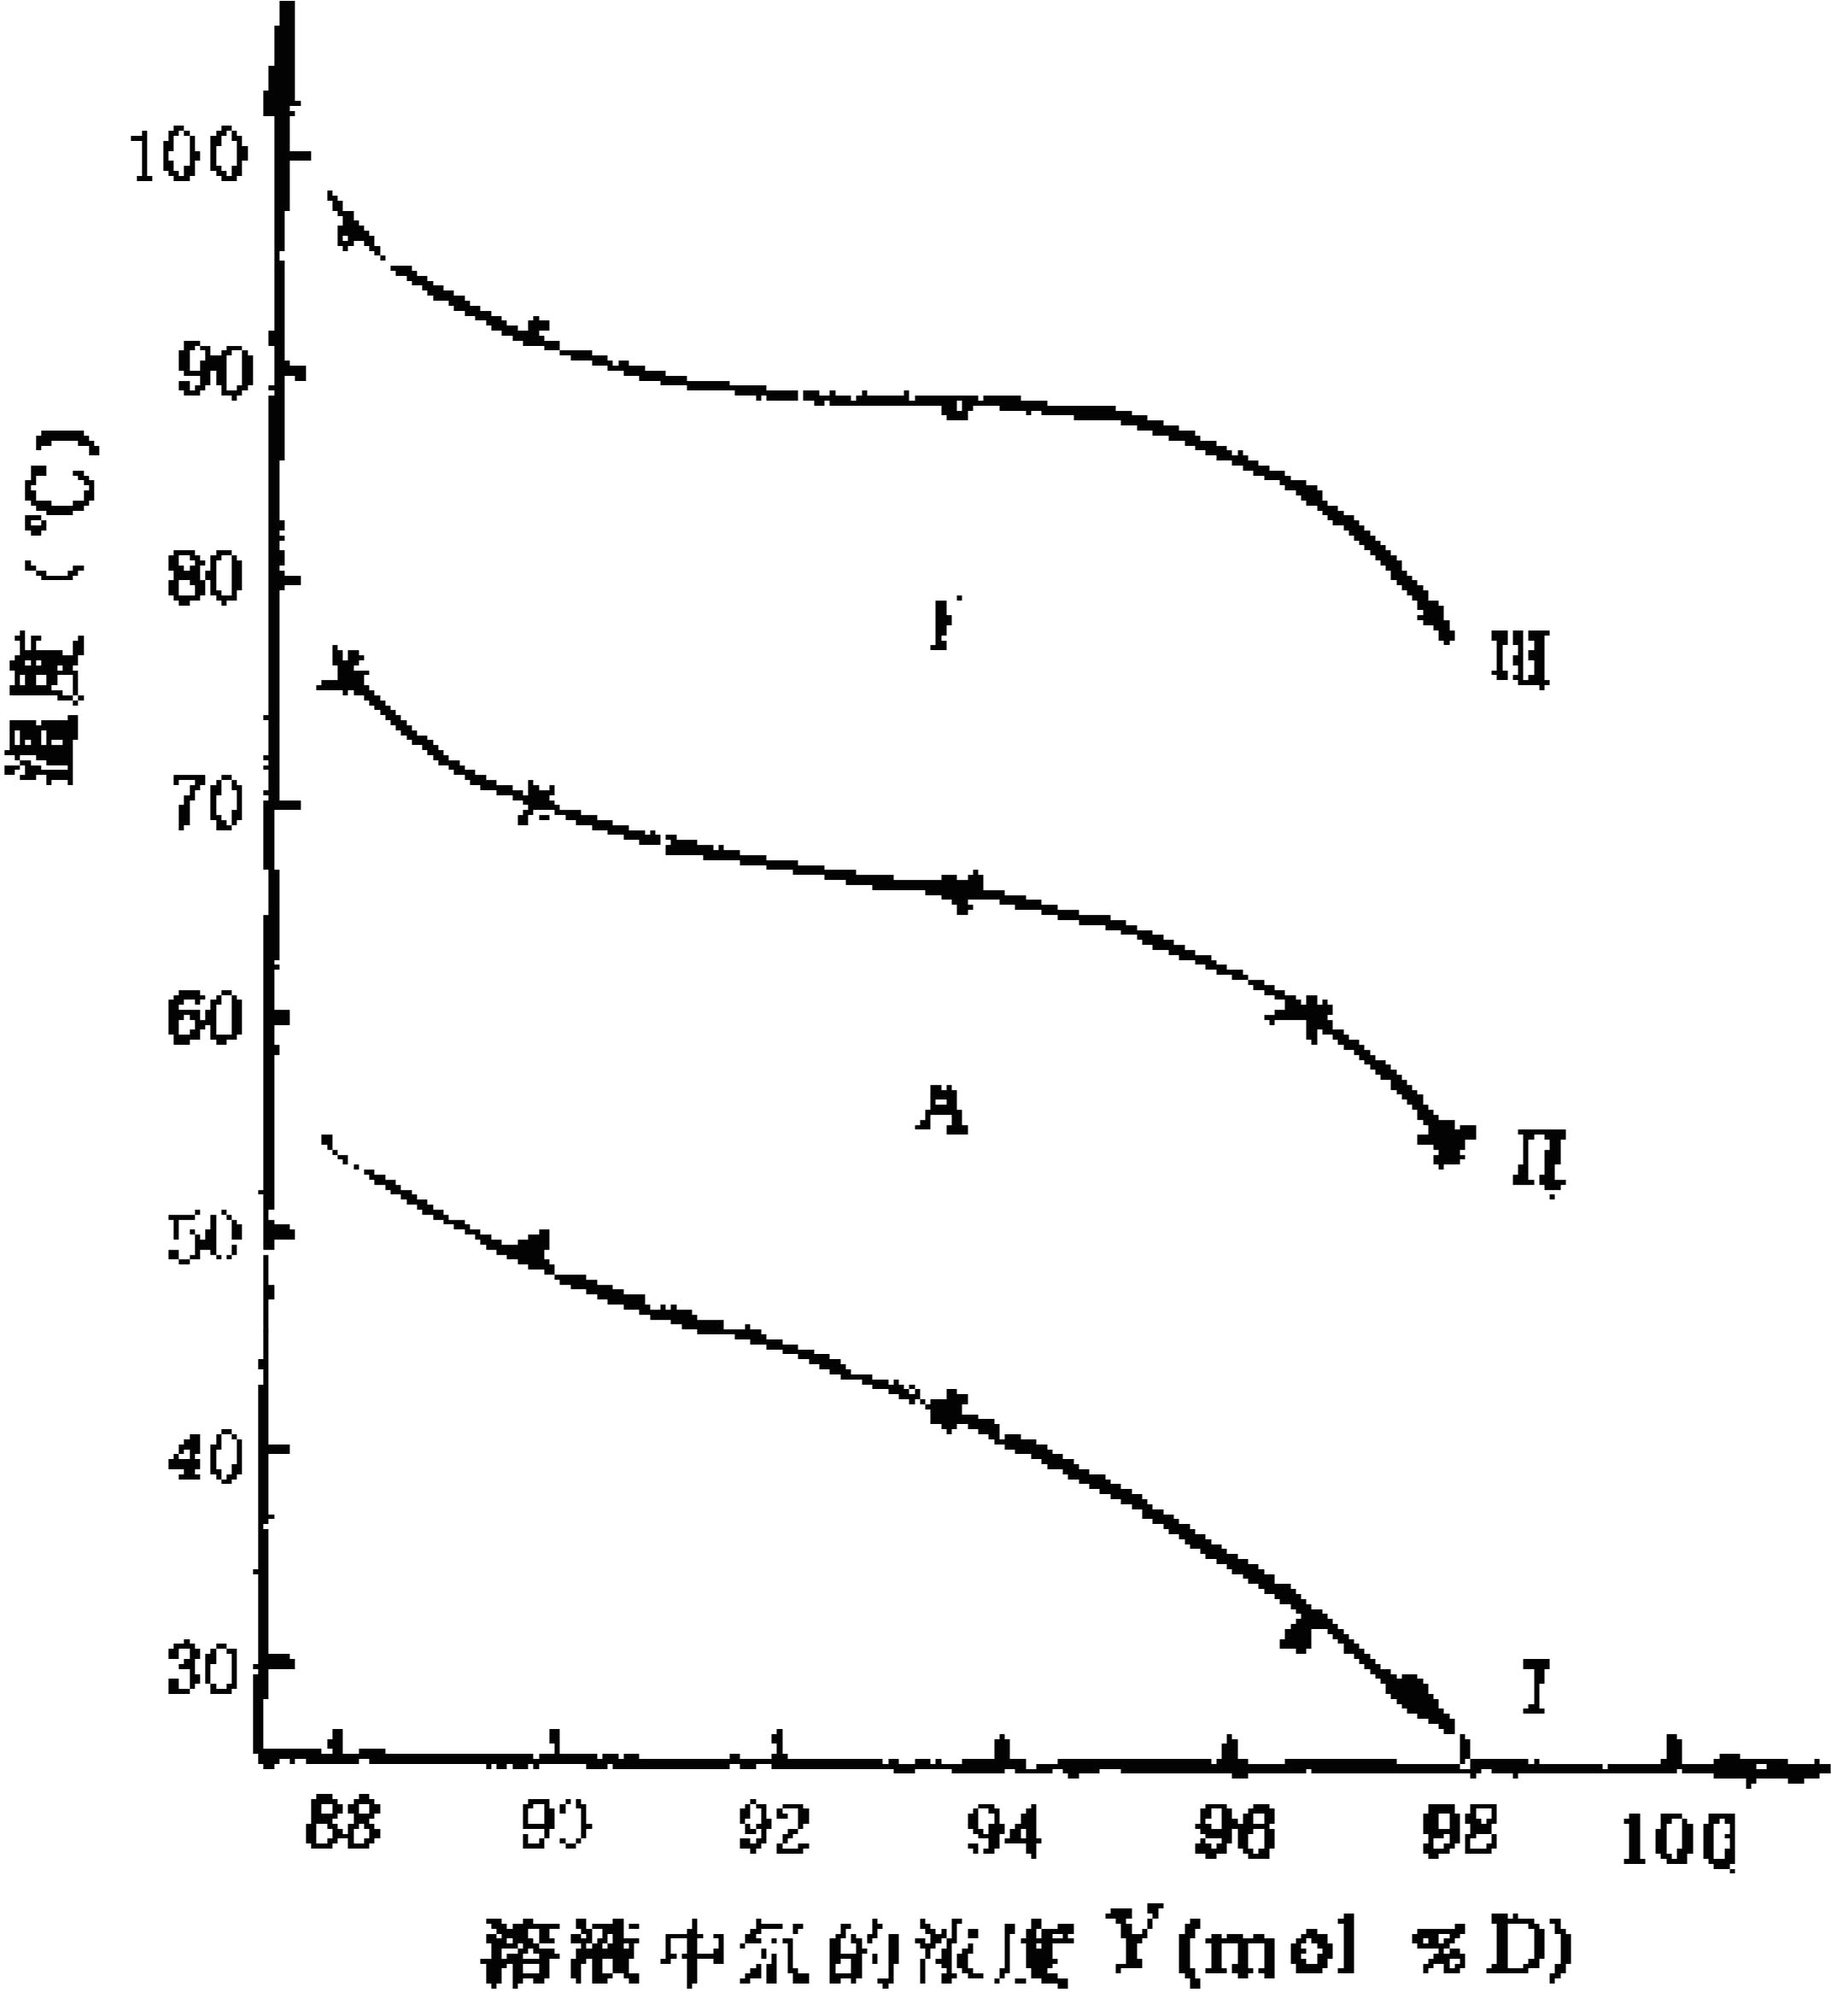
\includegraphics[width=0.8\textwidth]{fig/cp03/img3.16.jpg}
 \caption{四方和单斜DKDP的稳定区。}
\end{figure}

当溶液温度偏离转变点时,只能存在一种晶相与溶液平衡,另一种晶相将被溶解。但是晶体生长过程是一个不平衡的过程。如果溶液状态点处于两相溶解度曲线以上,如图3.15中的F点,则溶液对EDT无水物和水合物都是过饱和的,两相都可以生长,但无水物是稳定相,水合物是亚稳相,溶液相对于前者过饱和度较大,故生长速度也快。如果状态点在E,则EDT水合物生长,无水物溶解。但如果在无水物的稳定区内引入水合物籽晶,则水合物晶体即可在该区内实现亚稳相生长,长成$\rm EDT\cdot H_2O$大晶体,前提条件是溶液的过饱和度能满足$\rm EDT\cdot H_2O$晶体生长而又不致引起EDT稳定相自发成核。这是完全可能的,因为自发成核所需的过饱和度要比晶种上生长所需的过饱和度大得多。亚稳相生长区的界限可通过实验求出。不同物质和不同相的亚稳相生长区是不一样的。例如图3.14中,转变点以上,$\rm EDT\cdot H_2O$亚稳相生长区较窄(约6℃),而在转变点以下,EDT亚稳相生长区就较宽(约10℃)。对于DKDP,四方和单斜两相溶解度十分接近,亚稳相生长区比较宽,如对转变点为21℃的99.8\%的重水溶液,可以从43℃开始,用降温法成功地培养四方亚稳相晶体。图3.16粗略地示出在不同含氘量的重水溶液中,四方和单斜DKDP的亚稳相生长区。

溶液中的亚稳相晶体溶解度较大,在热力学上是不稳定的,它有自发地转变为溶解度较小的稳定相的趋势。例如,在离转变点较远的单斜稳定区中生长四方DKDP晶体时,在四方晶种上很容易长出单斜晶体,后者一旦出现即迅速生长,使四方母晶迅速被单斜晶体所“蚕食”。同样,在四方稳定区内生长单斜晶体时,也会出现四方晶体“蚕食”单斜母体的情况。

处于热力学不稳定状态的体系,在向其稳定状态过渡时,有时不是过渡到最稳定的状态(即自由能最低的状态),而是过渡到其自由能降低较小的中间状态。这一现象称为Ostwald阶段定律。例如在$\rm Na_2SO_4-H2O$体系中,有时从硫酸钠过饱和溶液中析出的不是稳定的$\rm Na_2SO_4\cdot 10H_2O$,而是亚稳相$\rm Na_2SO_4\cdot 7H_2O$(图3.14)。在DKDP的单斜稳定区中,有时也会析出亚稳的四方DKDP晶体(自发结晶实验证明,在图3.16上下两条虚线间析出的自发结晶既有单斜相,也有四方相),使溶液状态停留在亚稳四方相溶解度曲线附近,而不是直接降到单斜相溶解度曲线附近,虽然后者自由能降低更多,更为稳定。这样就有可能把溶液保持在中间状态,在这样的过饱和溶液中引入亚稳相籽晶,常常可以达到生长亚稳相晶体的目的。

在亚稳的条件下,生长亚稳相晶体有许多优点。许多高温变体如能在较低的温度下作为亚稳相自溶液中生长,则具有在本章开始时所述的优越性。在另一些情况下,由于某一相稳定区的局限性,需要在另一相的稳定区内生长。例如在氘化程度较高的重水溶液中,DKDP的转变温度很低,为了能在通常的温度区间用降温法生长出高含氘量的四方DKDP晶体,也可以在起始温度适当高于转变温度的情况下,使该晶体在单斜相稳定区内生长。图3.17示出的四方DKDP大晶体就是在这样的条件下生长出来的。在育晶器底部可以清楚地看见在生长过程中自发形成的单斜杂晶,由于溶液对这两相都是过饱和的,所以四方相和单斜相能同时存在和生长(但溶液和这两相并不处于平衡状态)。由此可见,亚稳相晶体生长的研究,在理论和实践上都是很有意义的。

\begin{figure}[h]
 \centering
 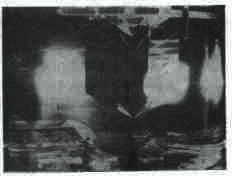
\includegraphics[width=0.8\textwidth]{fig/cp03/img3.17.jpg}
 \caption{在单斜相稳定区内生长的DKDP大晶体($\rm 5.7\times 5.7\times 4.5cm$)}
\end{figure}

 %相稳定区和亚稳相生长
\setcounter{section}{2}
\section{从溶液中生长晶体的方法}
从溶液中生长晶体过程的最关键因素是控制溶液的过饱和度。使溶液达到过饱和状态,在晶体生长过程中维持其过饱和度的途径有:
\begin{enumerate}[(1)]\itemsep -0.5ex
\item 据溶解度曲线,改变温度。
\item 采取各种方式(如蒸发、电解)移去溶剂,改变溶液成分。
\item 通过化学反应来控制过饱和度。由于化学反应速度和晶体生长速度差别很大,做到这一点是很困难的,需要采取一些特殊的方式,如通过凝胶扩散使反应缓慢进行等。
\item 用亚稳相来控制过饱和度,即利用某些物质的稳定相和亚稳相的溶解度差别,控制一定的温度,使亚稳相不断溶解,稳定相不断生长。
\end{enumerate}

根据晶体的溶解度和温度系数,从溶液中生长晶体的具体方法有下述几种。

\subsection{降温法}
降温法是从溶液中培养晶体的一种最常用的方法。这种方法适用于溶解度和温度系数都较大的物质,并需要一定的温度区间。这一温度区间也是有限制的:温度上限由于蒸发量大而不宜过高,当温度下限太低时,对晶体生长也不利。一般来说,比较合适的起始温度是50---60℃,降温区间以15---20℃为宜。

降温法的基本原理是利用物质较大的正溶解度温度系数,在晶体生长过程中逐渐降低温度,使析出的物质不断在晶体上生长。用这种方法生长的物质的溶解度温度系数最好不低于1.5g/1000g$\text{溶液}\cdot$℃,表3.7列出符合此要求的一些物质的数据。

\begin{table}[h]
\centering
\caption{40℃时,一些物质的溶解度及其温度系数}
\begin{tabular}{c|c|c}\toprule
物质 & \tabincell{c}{溶解度\\(g/1000g溶液)} & \tabincell{c}{溶解度温度系数\\g/1000g$\text{溶液}\cdot$℃}\\\hline
明矾\quad$\rm K_2SO_4\cdot Al_2(SO_4)_3\cdot 24H_2O$ & 240 & $+9.0$\\
ADP\quad$\rm NH_4H_2PO_4$ & 360 & $+4.9$\\
TGS\quad$\rm (NH_2CH_2COOH)_3\cdot H_2SO_4$ & 300 & $+4.6$\\
KDP\quad$\rm KH_2PO_4$ & 250 & $+3.5$\\
EGT\quad$\rm ???$ & 598 & $+2.1$\\
\bottomrule
\end{tabular}
\end{table}

降温法生长晶体的几种装置,如图3.18、图3.19和图3.20所示。

在降温法生长晶体的整个过程中,必须严格控制温度,并按一定程序降温。研究表明,微小的温度波动就足以在生长的晶体中造成某些不均匀区域。为提高晶体生长的完整性,要求控温精度尽可能高(目前已达±0.001℃),此外还需造成适合晶体生长的其他条件。

\begin{figure}[h]
 \centering
 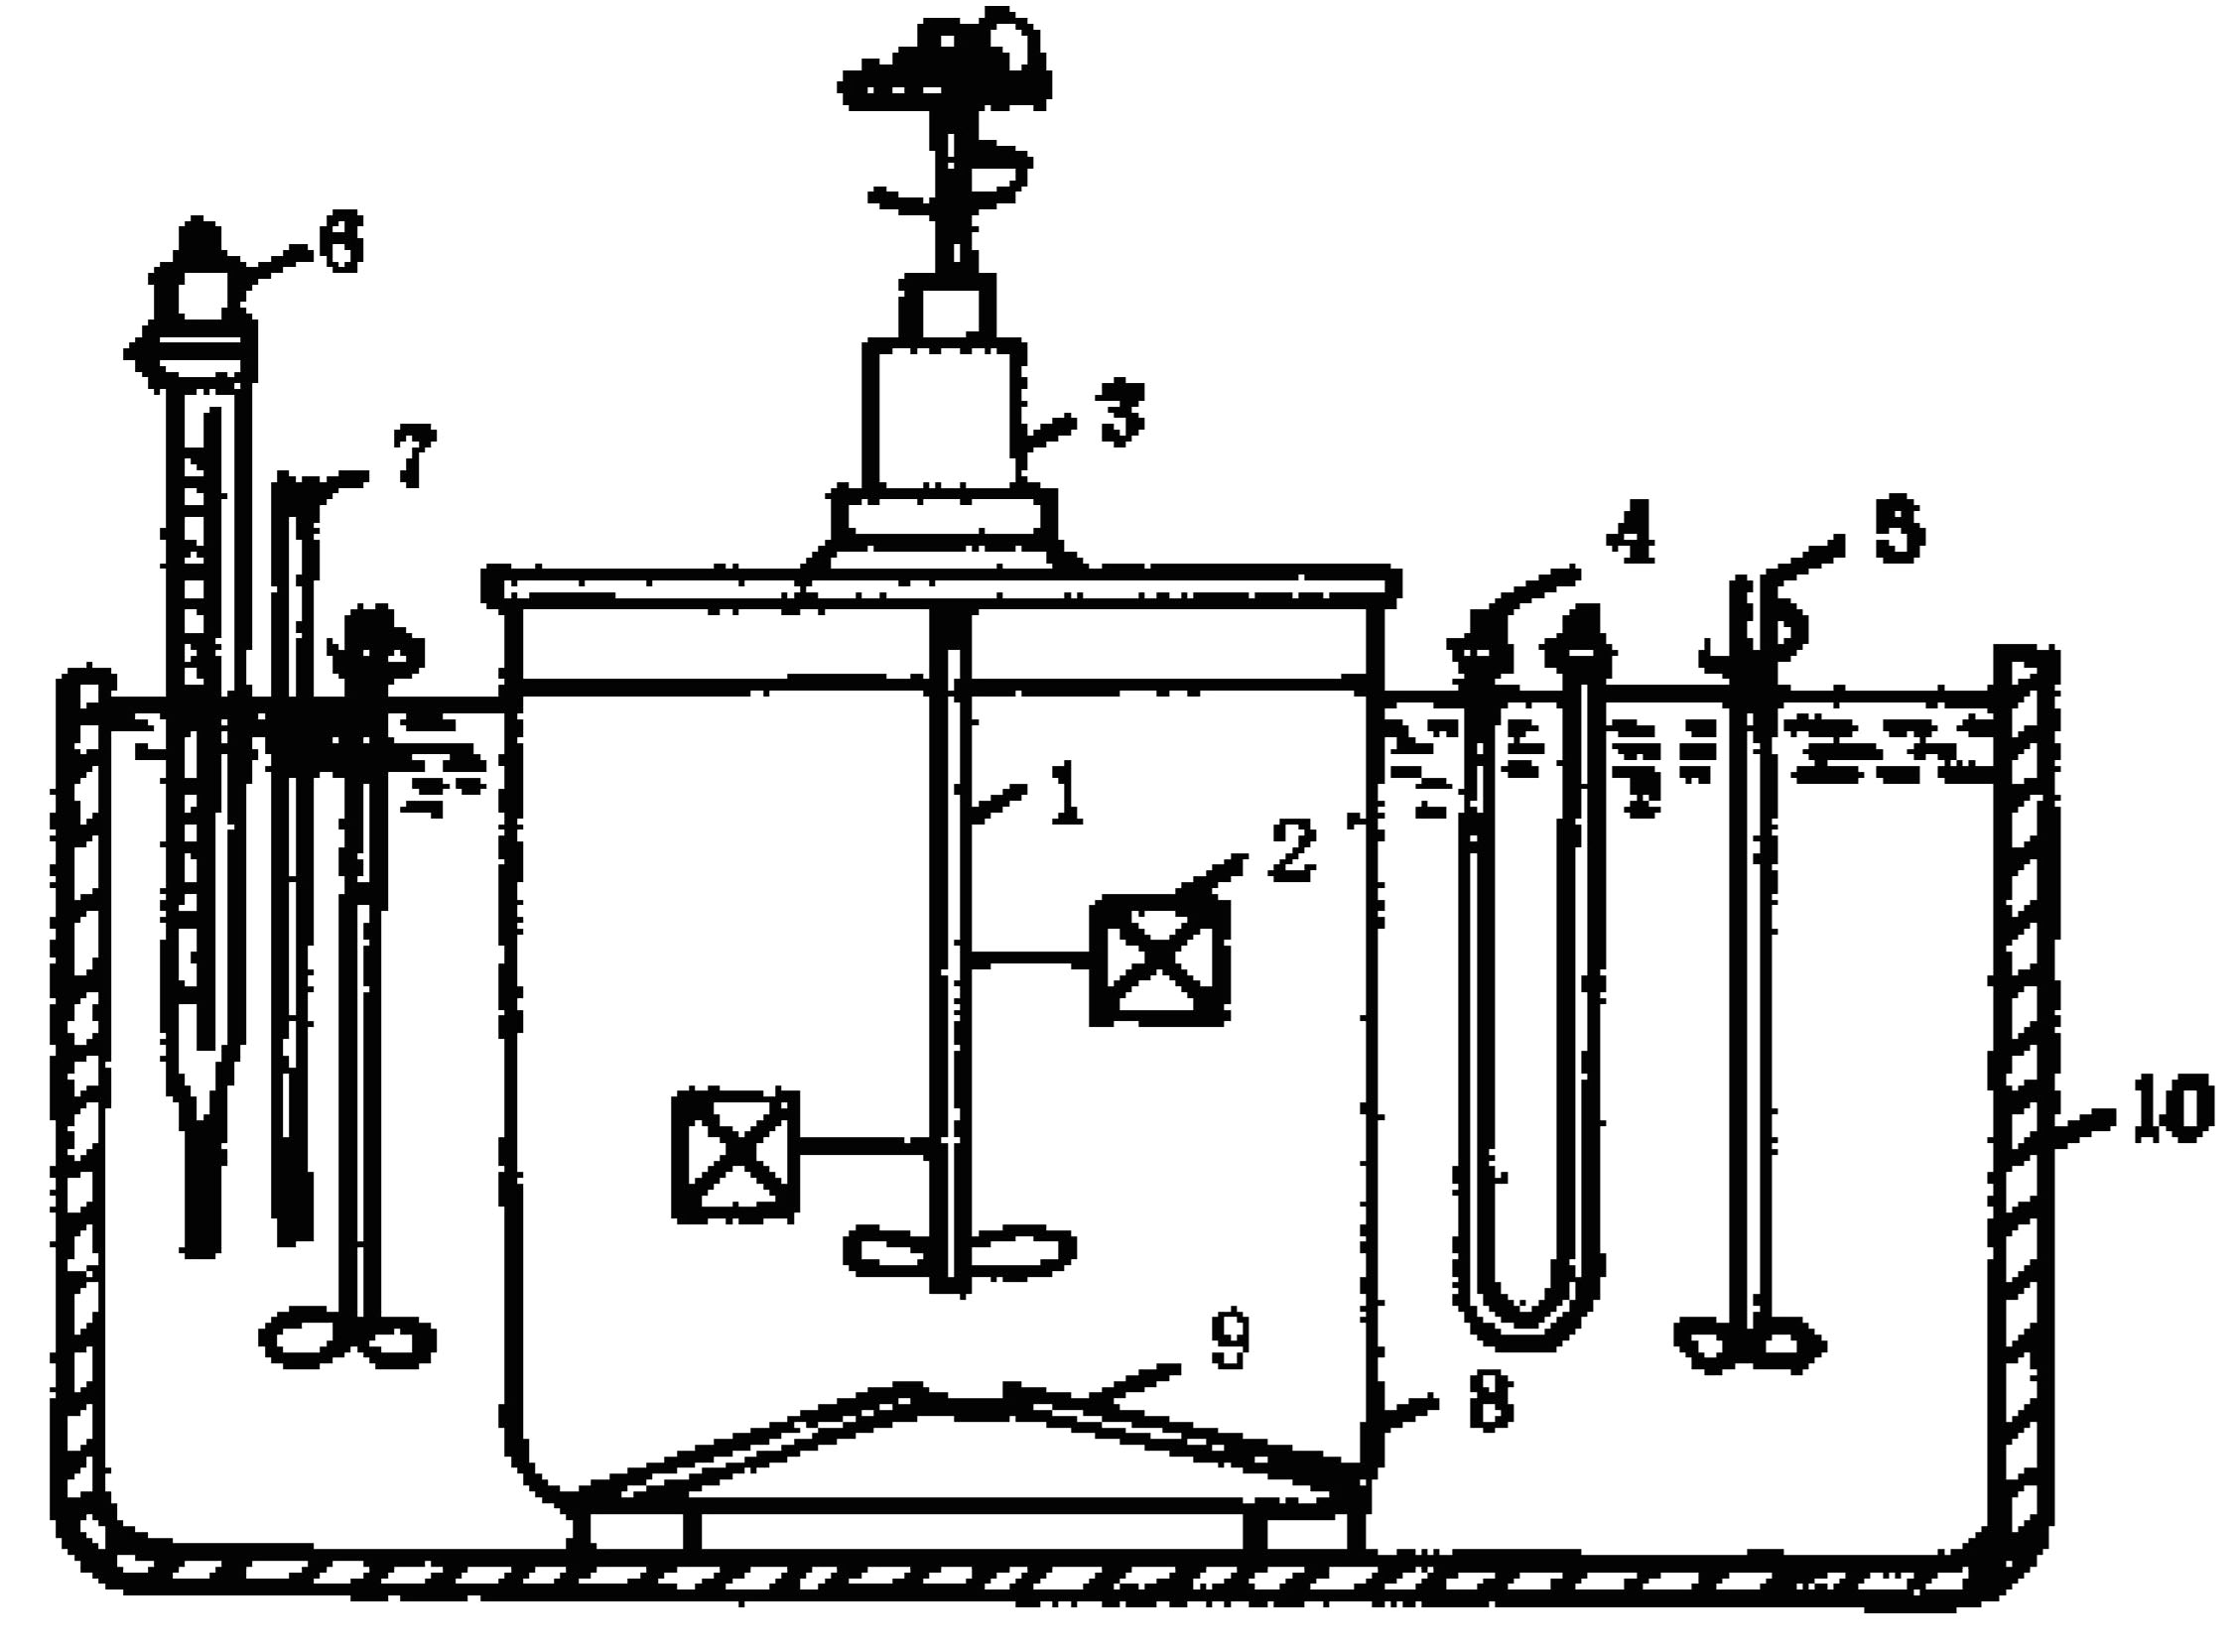
\includegraphics[width=0.5\textwidth]{fig/cp03/img3.18.jpg}
 \caption{水浴育晶装置。图中:}
 1为掣晶杆;2为晶体;3为转动密封装置;4为浸没式加热器; \\
 5为搅拌器;6为控制器(接触温度计);7为温度计;8为育晶器;\\
 9为有孔隔板;10为水槽。
\end{figure}

在利用降温法来生长晶体的过程中可不用再补充溶液或溶质。因此,整个育晶器在生长过程中必须严格密封,以防溶剂蒸发和外界的污染。例如从重水溶液中生长晶体时,如果密封不好,溶液中的D$_2$O就会同大气中的H$_2$O汽发生同位素交换而使溶液氘化程度下降。为增加温度的稳定性,育晶器的容量必须要大些(大型育晶器有几十升至上千升),加热保温方式有水浴槽或内部加热、外壳加保温套等。育晶器顶部经常有保持冷凝水回流,底部有电炉加热为好,使得溶液表面和底部都有不饱和层保护,避免自发晶核形成。

育晶器内的控温精度除了与育晶装置的结构有关外,很大程度上取决于控温装置,继电器开关式控温一般可以满足水溶液晶体生长的要求,温度波动可以控制在±0.05℃以下,用PID控温方式,特别是使用可编程温度控制器控温,实现控温精度至±0.005℃并不困难,这对培养高完整性单晶十分有利。

\begin{figure}[htb]
 \centering
 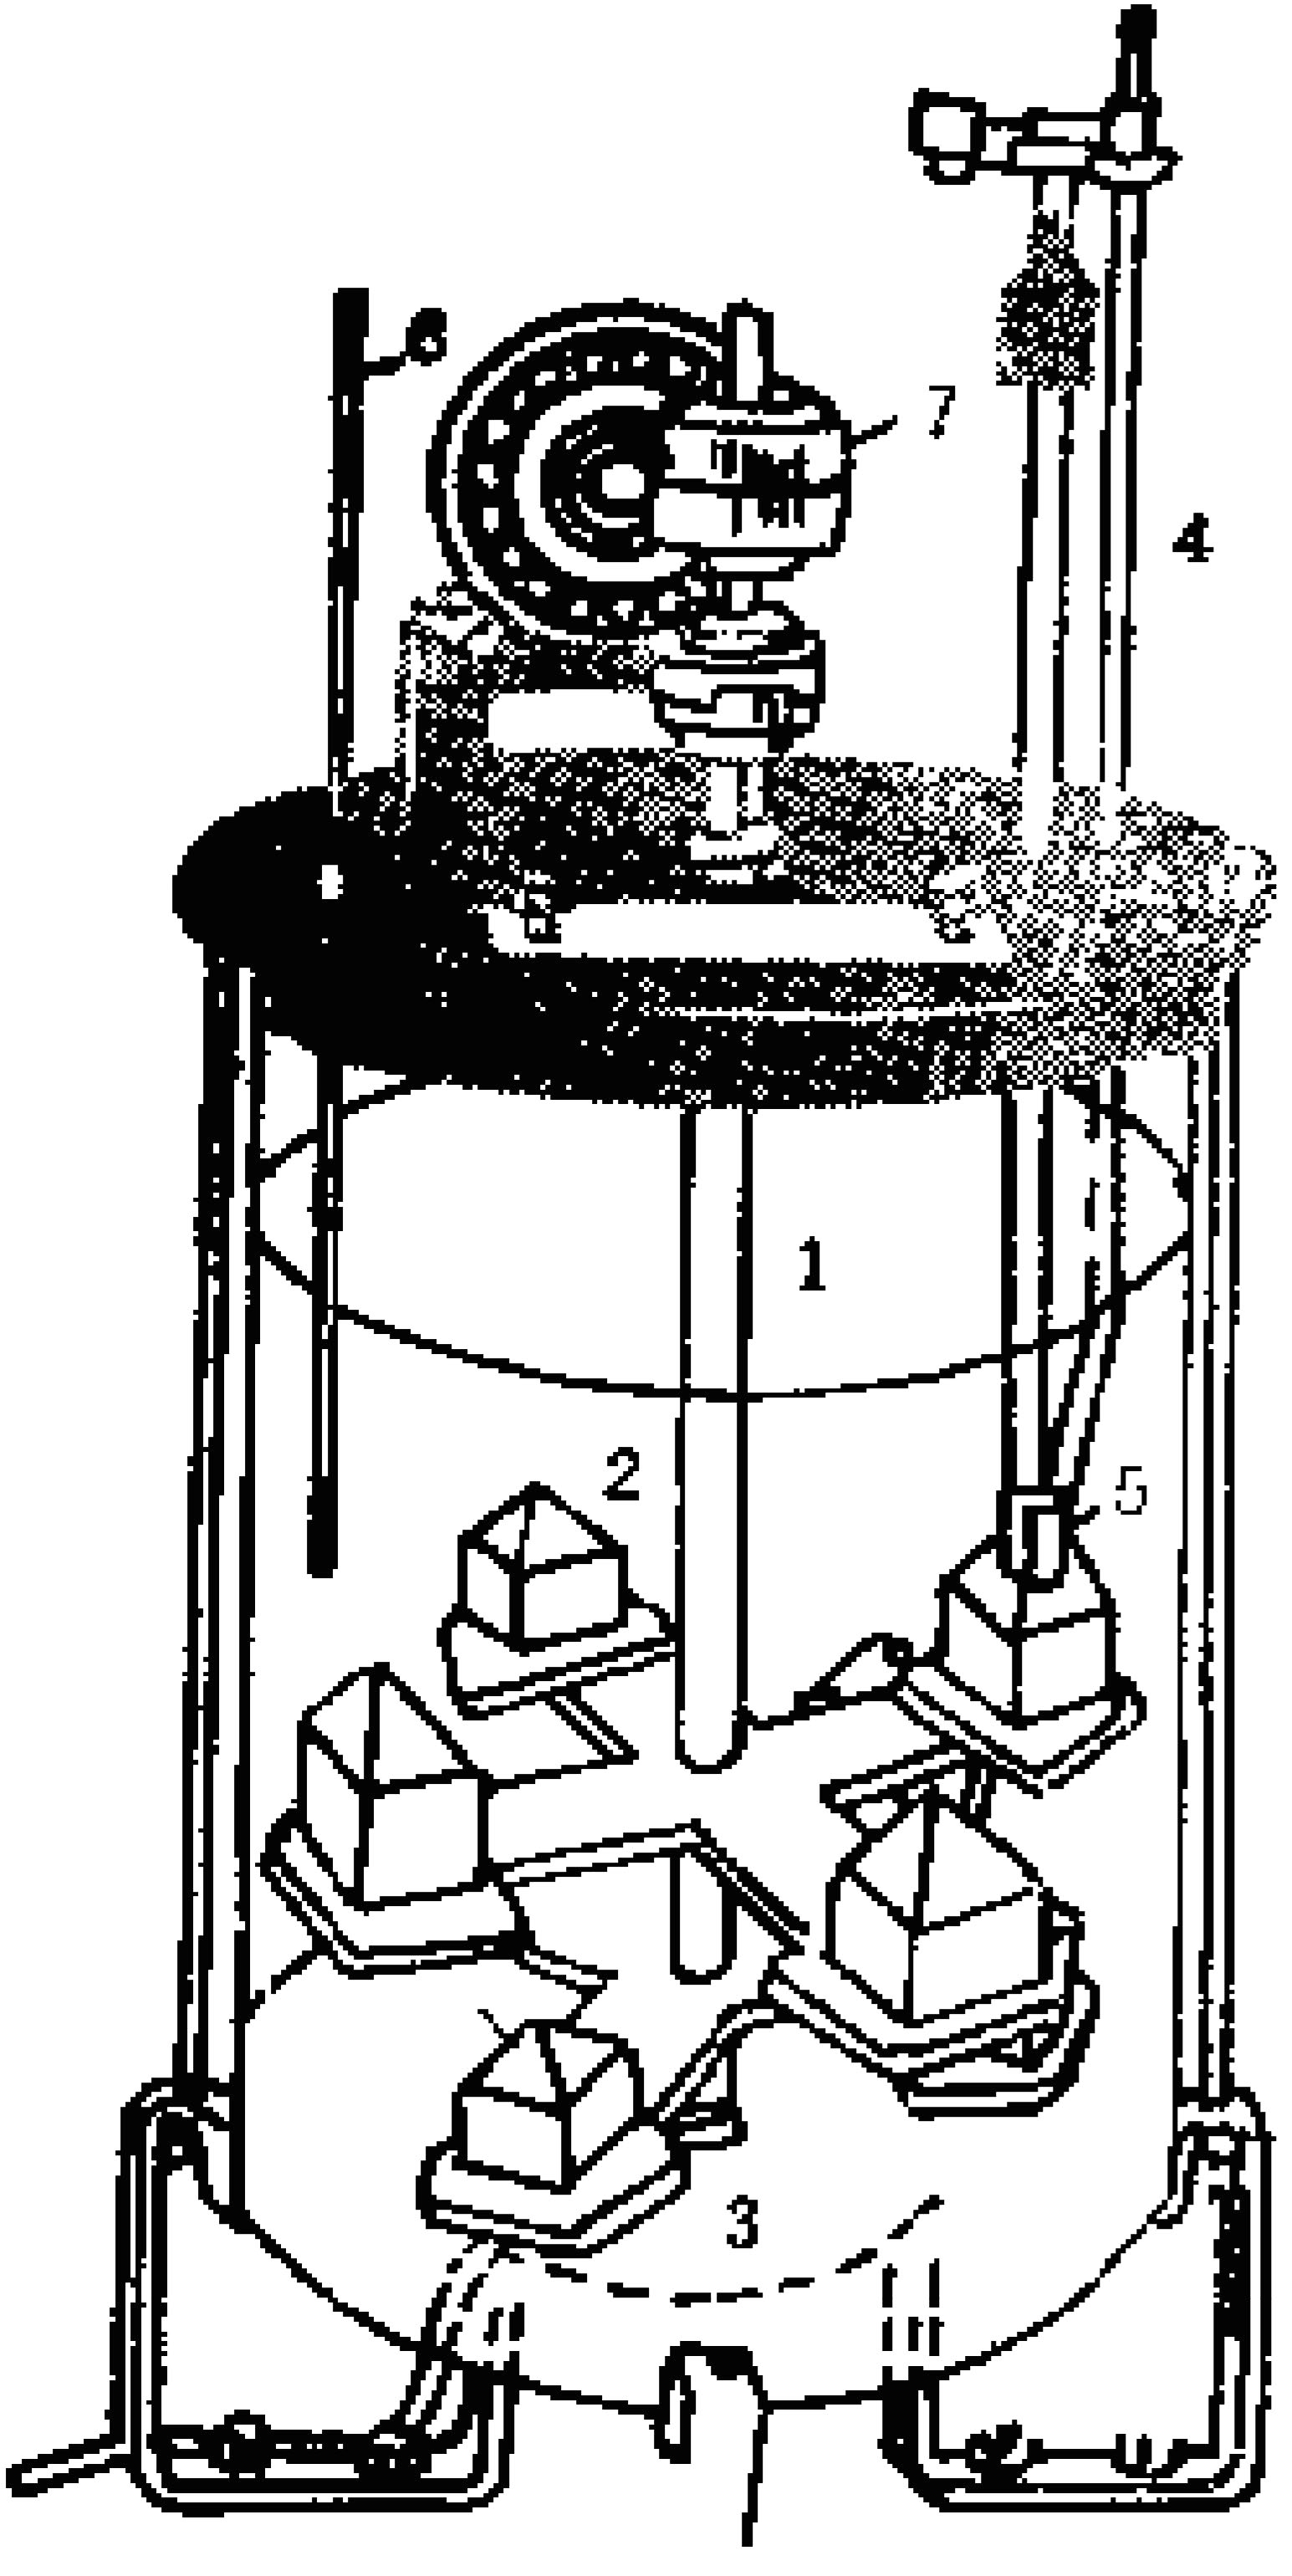
\includegraphics[width=0.3\textwidth]{fig/cp03/img3.19.jpg}
 \caption{直接加热的转动育晶器。}
 图中:1为掣晶板;2为晶体;3为底部主加热器;4为控制器; 5为辅助小灯泡加热器;6为温度计;7为可逆转动装置(30r/min)。
\end{figure}

\begin{figure}[htb]
 \centering
 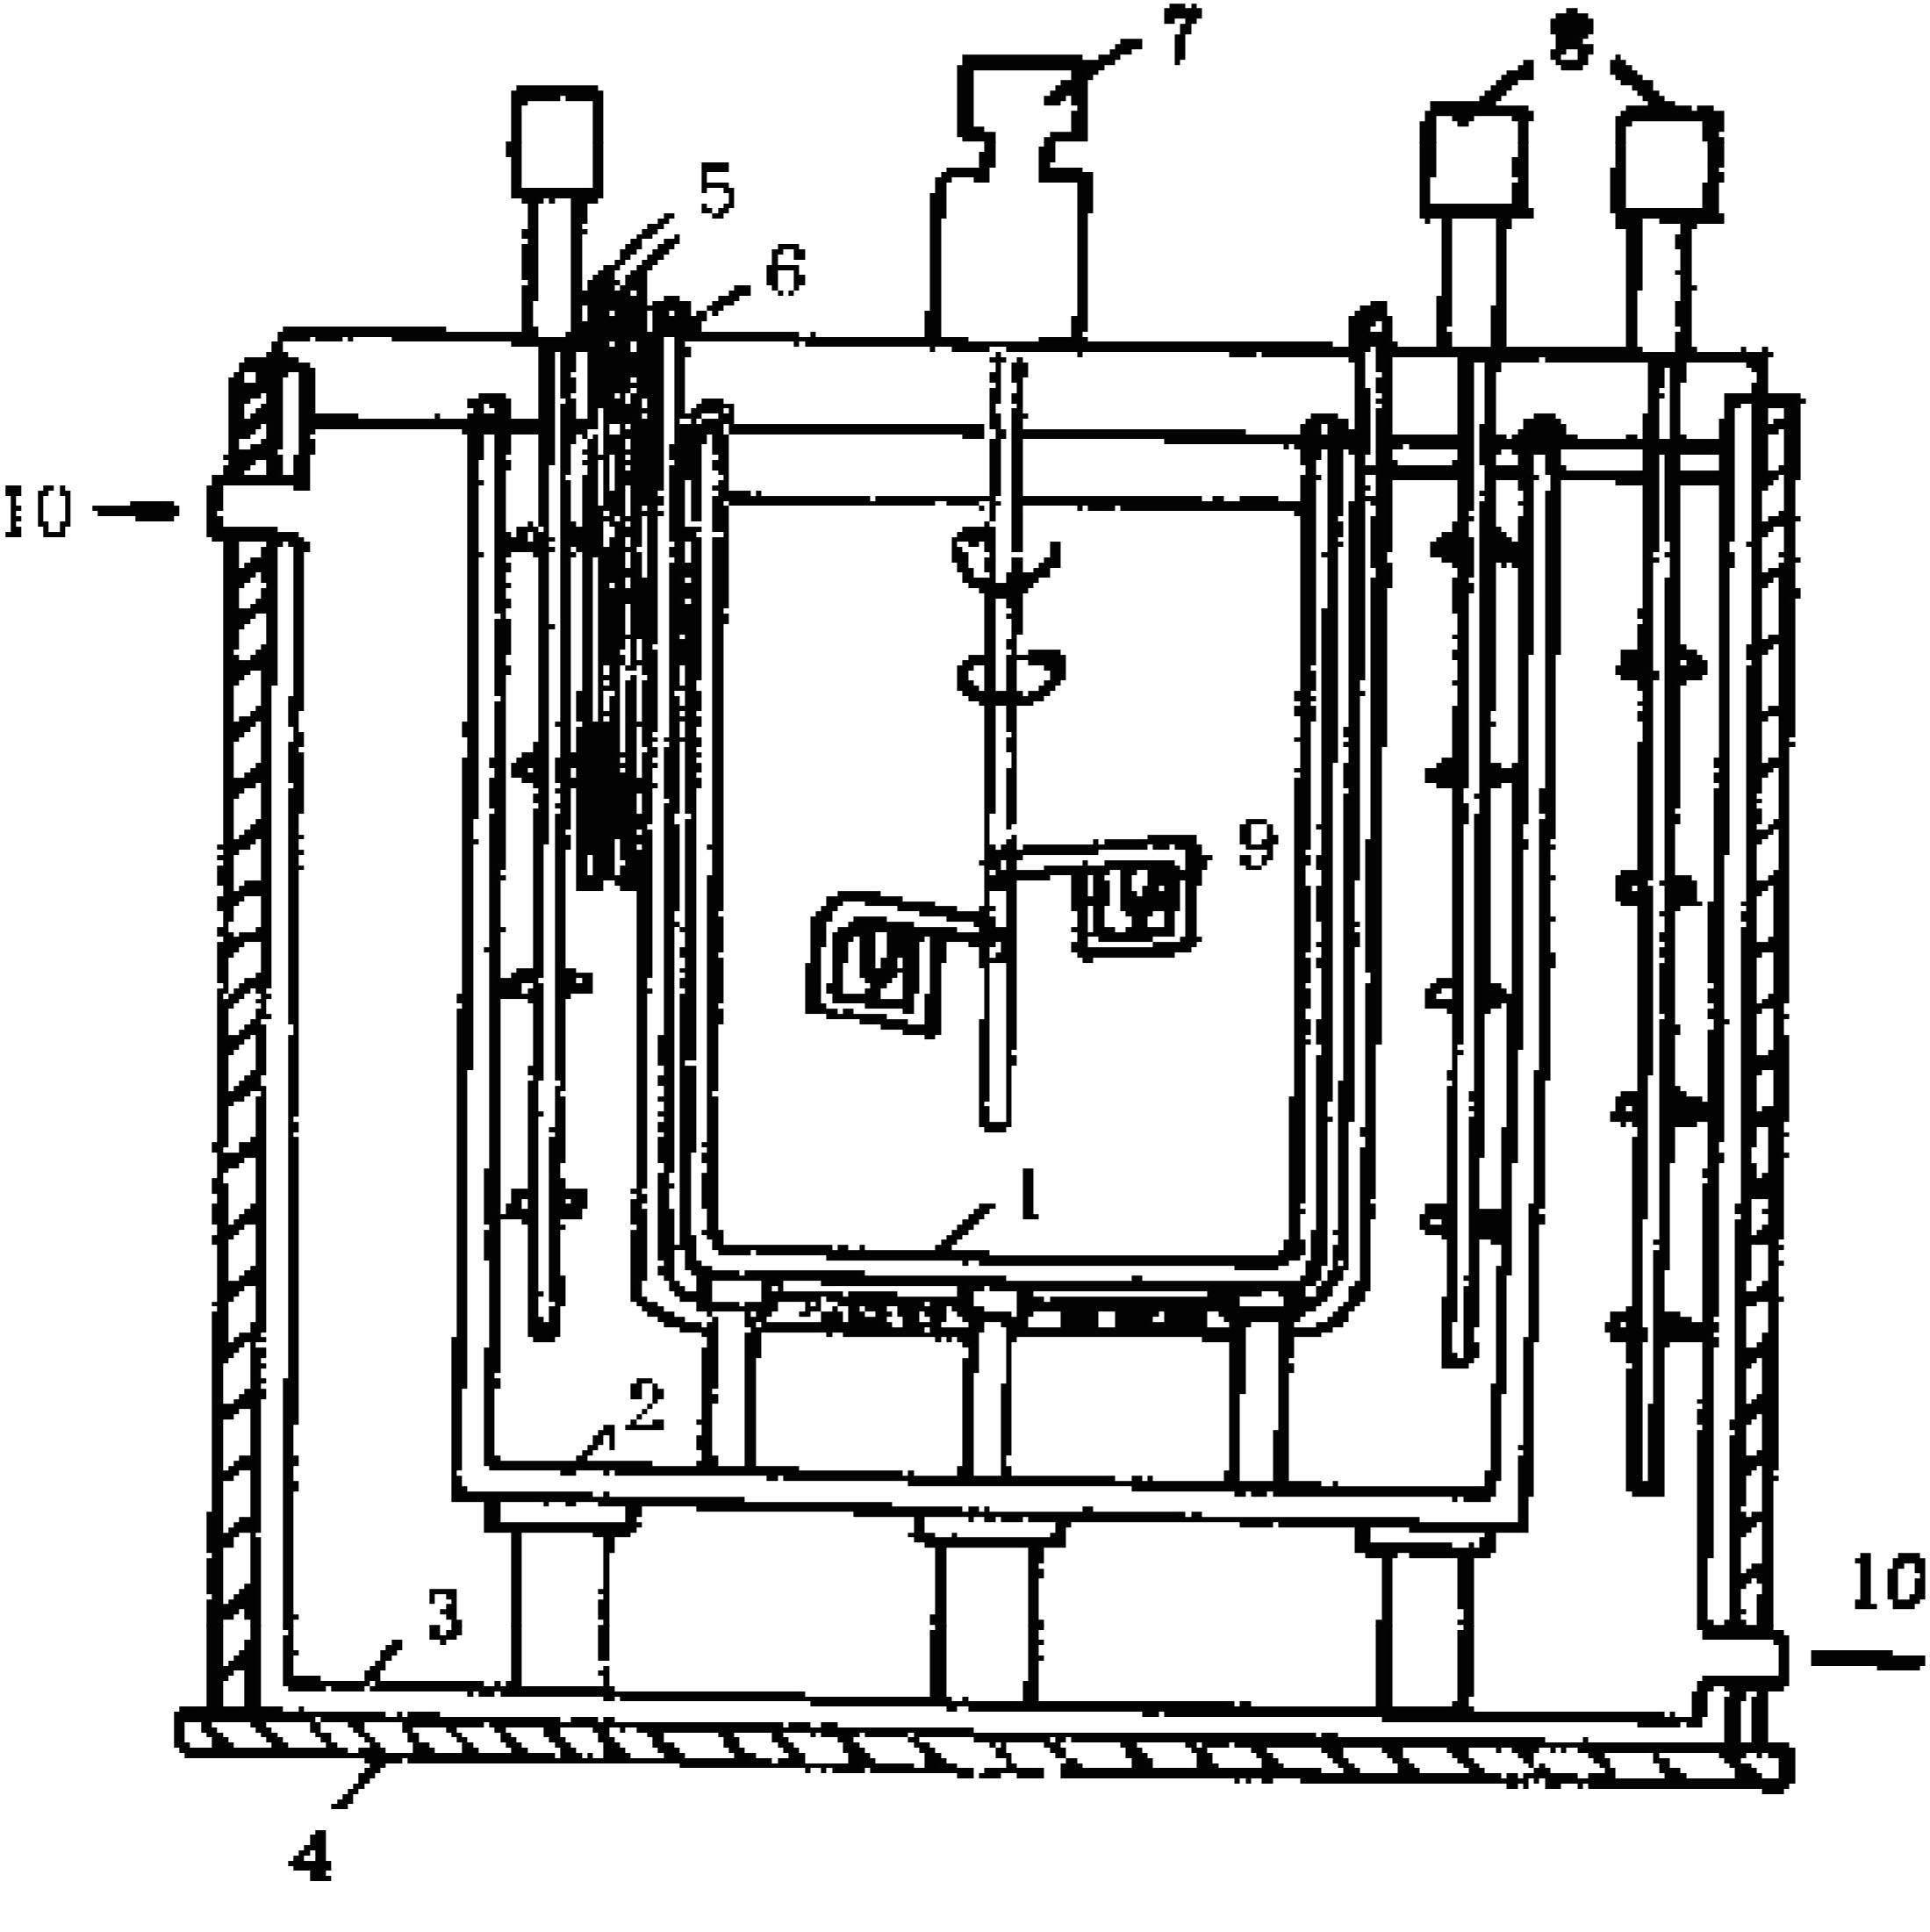
\includegraphics[width=0.45\textwidth]{fig/cp03/img3.20.jpg}
 \caption{双浴槽育晶装置。图中:}
 1为育晶器;2为内浴槽;3为外浴槽;4为保温层;5为感温元件;6为加热元件;7为转晶马达;8为搅拌马达(1500r/min);9为籽晶;10为外接冷却装置的进出口。
\end{figure}

为使溶液温度均匀,并使生长中的各个晶面在过饱和溶液中能得到均匀的溶质供应,要求晶体对溶液作相对运动。这种运动可采取多种形式,如晃动法(晶体固定不动,摇晃整个育晶器)、转晶法(晶体在溶液中作自转,公转或行星式转动)等,其中以晶体在溶液中自转或公转最为常用。为了克服这种方式所造成的的某些晶面迎液而动和使另一些晶面总是背向液流的缺点,转动需要定时换向,即用以下程序进行控制:正转---停转---反转---停转---正转。

降温法控制晶体生长的主要关键是掌握合适的降温速度。使溶液始终处于亚稳区内,并维持适宜的过饱和度,降温速度一般取决于以下述几个因素:
\begin{enumerate}[(1)]\itemsep -0.5ex
\item 晶体的最大透明生长速度(即在一定条件下不产生宏观缺陷的最大生长速度)。这一数值对不同晶体是有明显差别的(和亚稳区大小有关),例如对硝酸钠(NaNO$_3$)晶体为1mm/d,酒石酸钾钠(KNT)晶体则可达5mm/d以上。对同一晶体该数值还和晶体尺寸有关。
\item 溶解度的温度系数。溶解度的温度系数不但随不同物质而异,而且对同一种物质在不同的温度区间也一样。例如KDP的溶解度曲线在高温部分(50---70℃)温度系数较大,在低温部分(30℃以下)则较小。
\item 溶液的体积V(ml)和晶体生长表面积S(cm$^2$)之比,简称体面比。有些晶体(如KDP型晶体)在生长过程中,生长面积基本不变,而有些晶体(如KNT)在各个方向上都生长,S在生长过程中则在不断增加。
\end{enumerate}

总之,上述三个因素对于不同晶体是有明显差别的;对同一种晶体,这些因素在生长过程中也是在变化的。因此必须从实际出发,对不同的晶体在不同的阶段制定不同的降温程序。一般来说,在生长初期降温要慢,到了生长后期可稍快些。掌握规律后,可按程序实行自动降温。

必须指出,无宏观缺陷的晶体不一定是高质量的晶体(见3.4.3节)。培养用于光学目的高完整性的单晶,其生长速度应当控制的更小一些。

在控制降温过程中,最好能随时测定溶液的过饱和度(见3.1.4节)。同时,一些晶体生长现象[如生长涡流的强弱,晶面相对大小的变化,次要面的出现和消失,晶面花纹(见3.4.3节)等]往往是溶液过饱和度偏高或偏低以及晶体均匀性将遭破坏的“信号”。这些现象也可作为估计过饱和度、控制降温速度的参考信号。 %降温法
\subsection{流动法(温差法)}
流动法生长晶体装置一般由三部分组成(图3.21):生长槽(育晶器)C,溶解槽A和过热槽B。三槽之间的温度是B槽的温度高于A槽的温度高于A槽的,而A槽的温度又高于C槽的,A槽中过剩的原料在不断地搅拌下溶解,使溶液在高于C槽的温度在饱和,然后经过滤器进入过热槽B。过热槽的温度一般高于生长槽温度5--10℃。可以充分溶解从溶解槽流入的微晶,以提高溶液的稳定性。经过过热后的溶液用泵打入生长槽C,C槽的溶液是过饱和的,保证晶体生长有一定的驱动力。由于晶体的生长,从而使变稀的溶液流到溶解槽溶解原料,使溶液重新达到饱和,溶液如此循环流动,晶体不断生长。晶体的生长速度受到溶液的流动速度和A,C两槽温差的控制。这种方法的优点是生长温度和过饱和度都固定。使晶体始终在最有利的温度和最合适的过饱和度下生长,避免了因生长温度和过饱和度变化而产生的杂质分凝不均匀和生长带等缺陷,使晶体完整性更好。流动发的另一个优点就是生长大批量的晶体和培养大单净不收溶解度和溶液体积的影响,只受生长容器大小的限制。日本大阪大学用这种方法长出400$\times$400$\times$600mm大KDP晶体,生长速度达2mm/d。流动法的缺点是设备比较复杂,调节三槽之间适当的温度梯度和溶液流速之间的关系需要有一定的经验。
\begin{figure}[h]
 \centering
 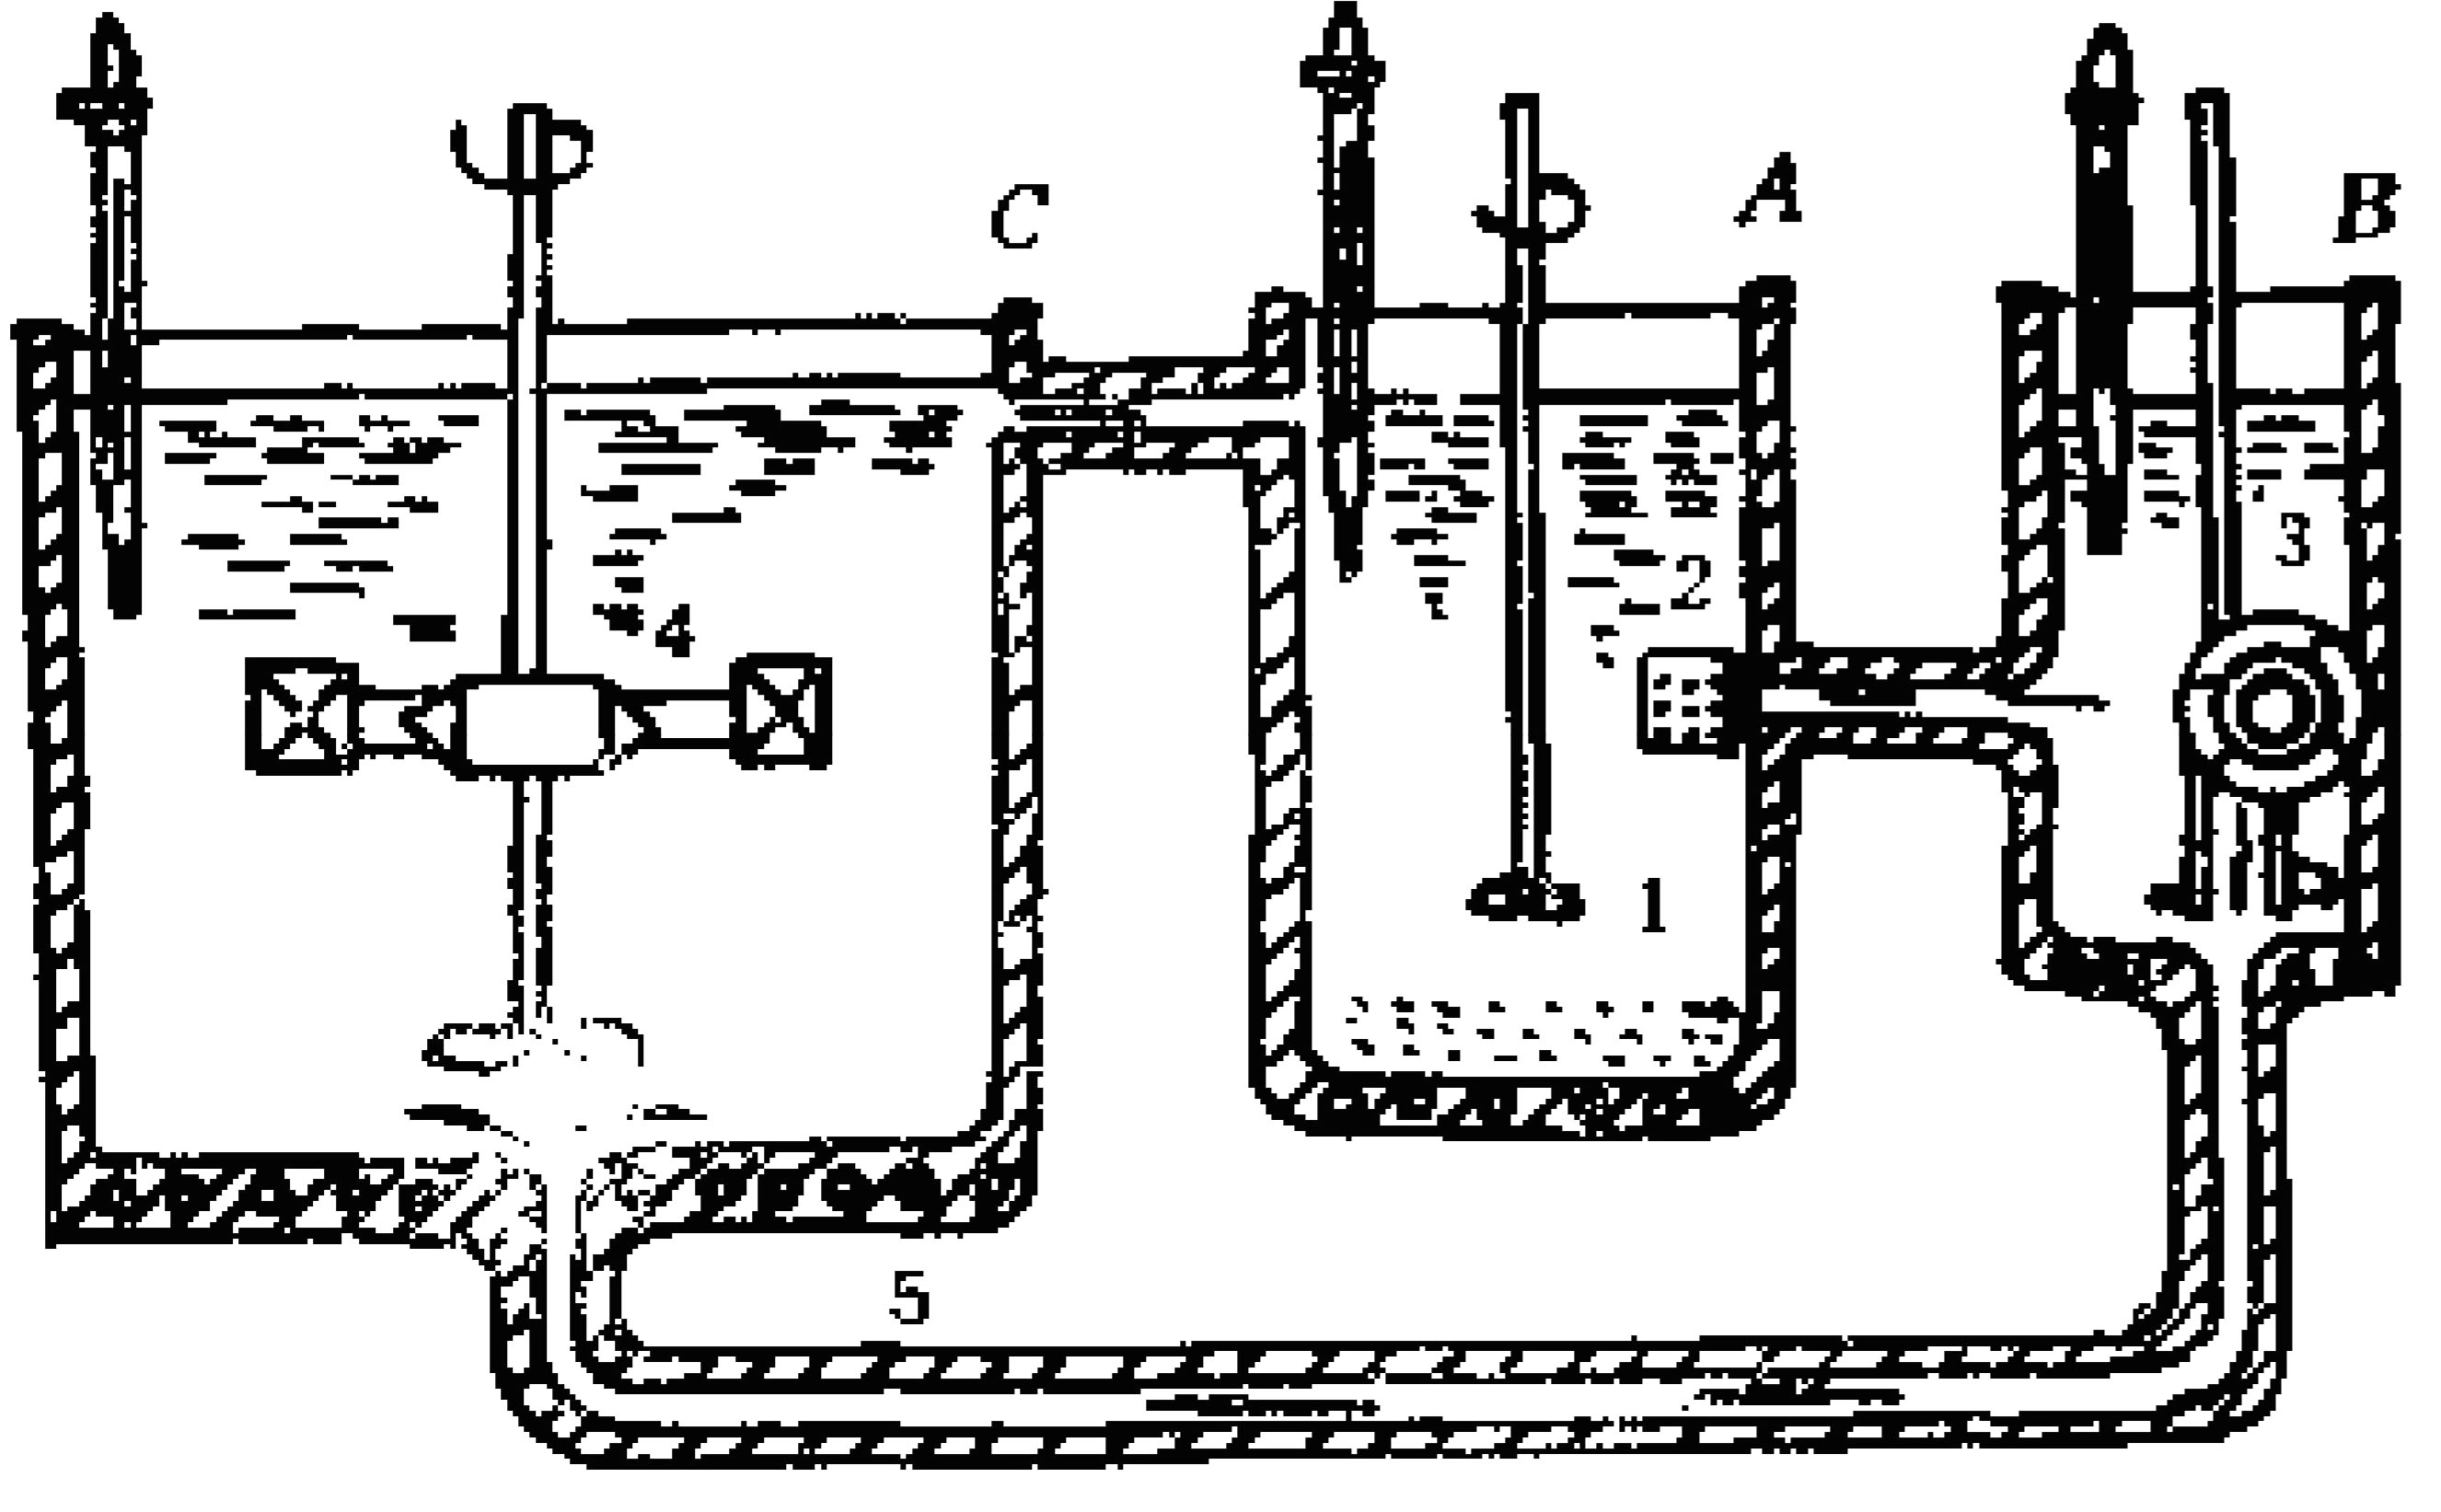
\includegraphics[width=0.6\textwidth]{fig/cp03/img3.21.jpg}
 \caption{循环流动育晶装置}
\end{figure}

采用适当装置也可以利用浓差自然对流来生长晶体。图3.22示出利用亚稳相和稳定相溶解度的差别通过浓差对流来生长$\alpha$-LiIO$_3$体的装置。两连通的玻璃槽,右边装$\beta$-LiIO$_3$原料,左边为生长槽,由于在20--30℃时,$\beta$-LiIO$_3$的溶解度比$\alpha$-LiIO$_3$的大1--2\%。浓度较大的LiIO$_3$溶液靠自然对流进入左边生长区,生长槽下部设置加热器,将溶液温度保持在40℃,造成对$\alpha$-LiIO$_3$的过饱和,析出的溶质在$\alpha$-LiIO$_3$种子上生长,变稀的溶液上升流回右边的原料槽重新溶解$\beta$-LiIO$_3$,原料槽靠空气冷却稳定在20--30℃。
\begin{figure}[h]
 \centering
 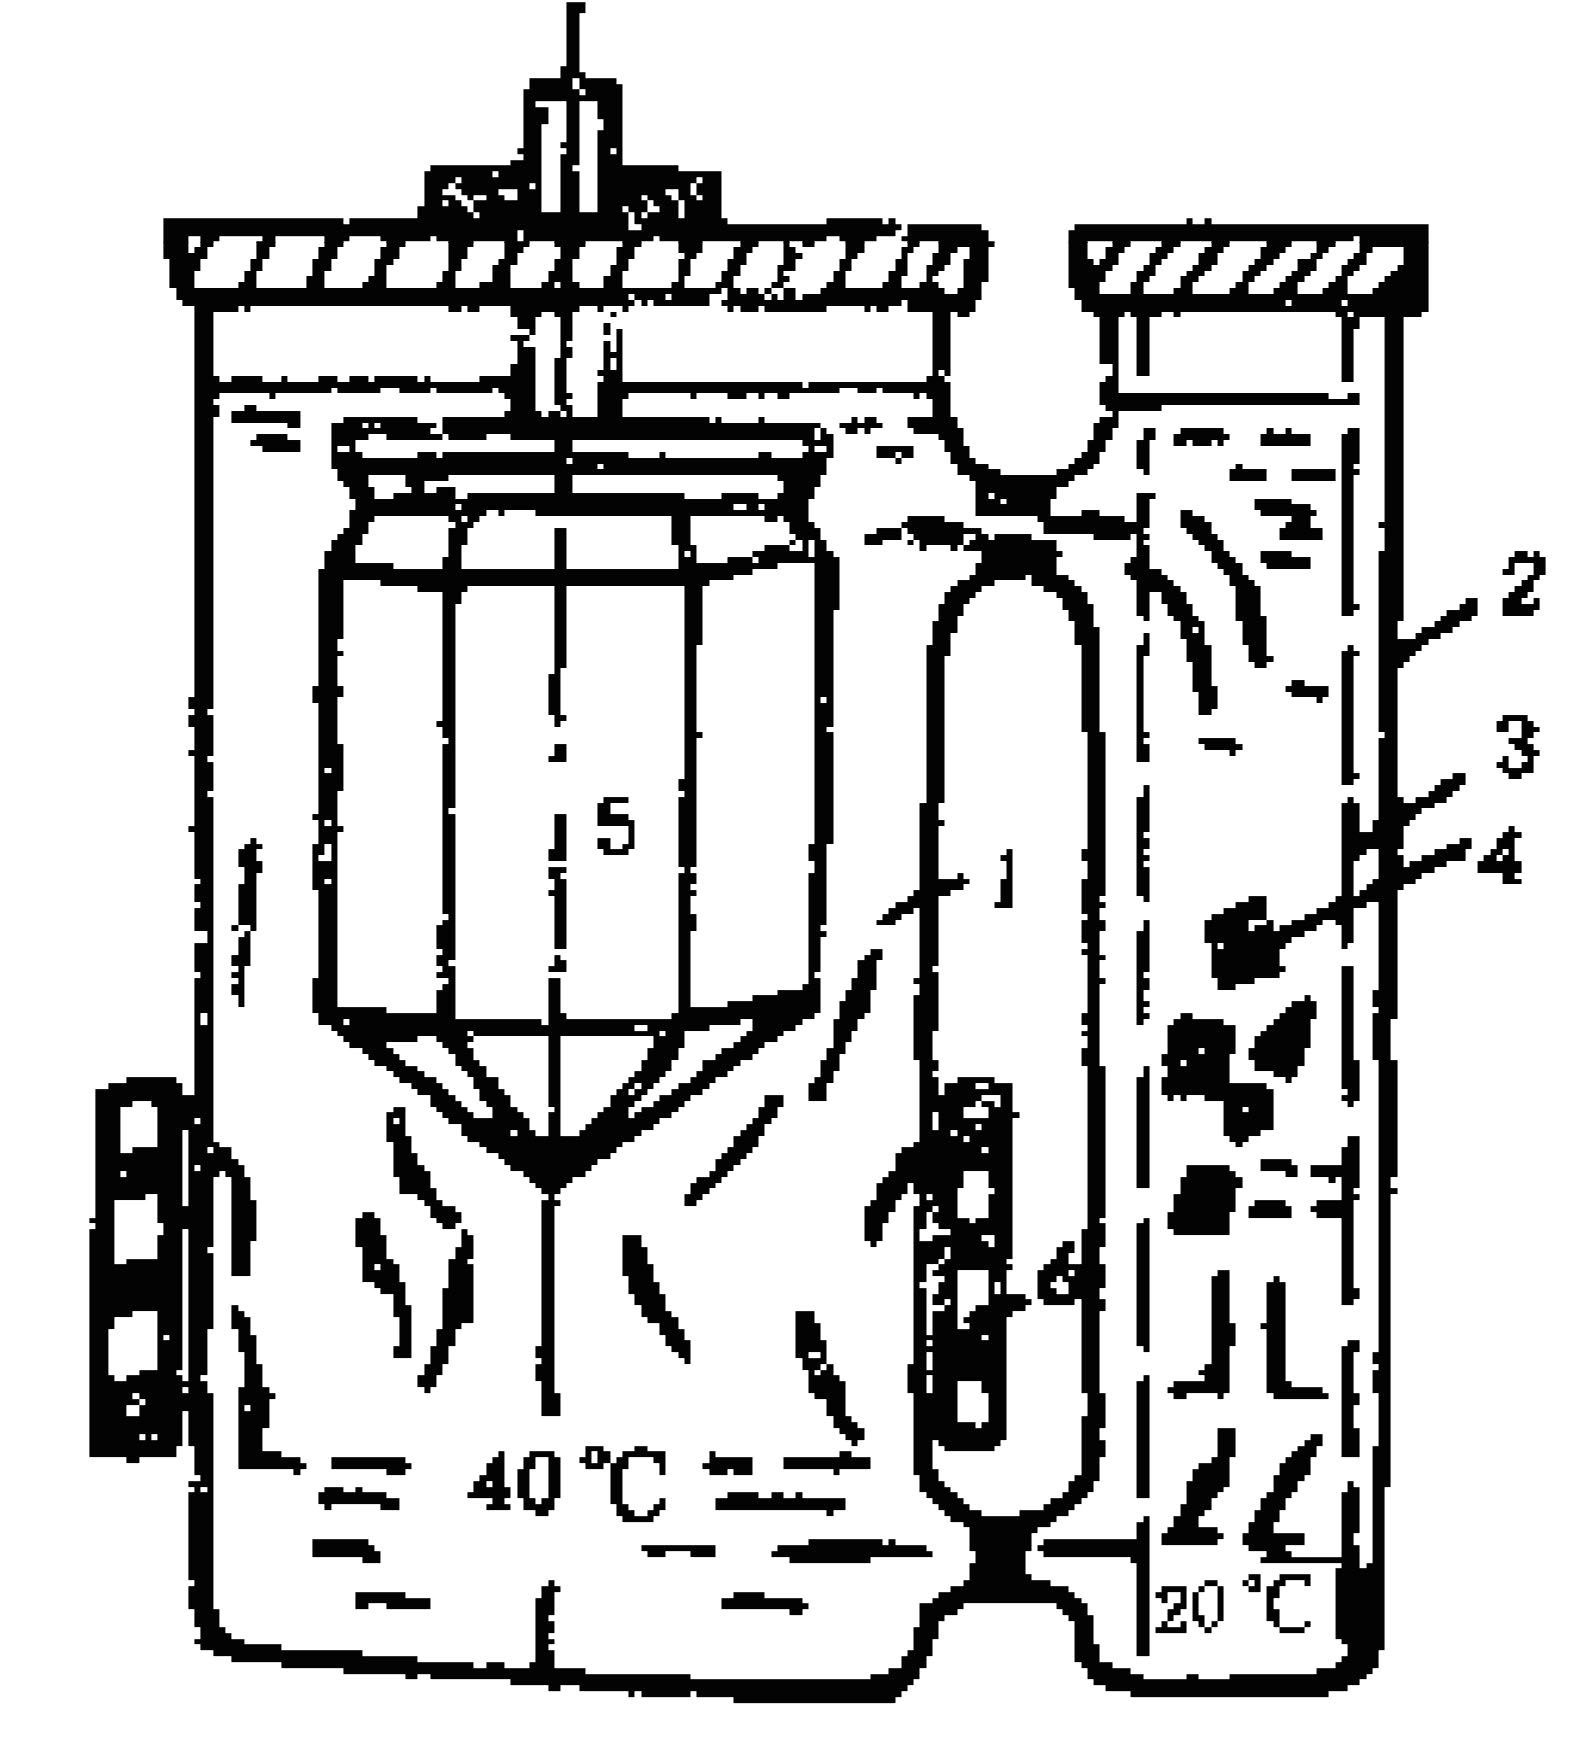
\includegraphics[width=0.5\textwidth]{fig/cp03/img3.22.jpg}
 \caption{浓差对流法生长LiIO$_3$晶体的装置}
\end{figure} %浓差法
\subsection{蒸发法}
蒸发法生长晶体的基本原理是将溶剂不断蒸发移去,而使溶液保持在过饱和状态,从而使晶体不断生长,这种方法比较适合于溶解度较大而其温度系数很小或是具有负温度系数的物质(表3.8)。蒸发法和流动法一样,晶体生长也是在恒温下进行的。不同是流动法用补充溶质,而蒸发法用移去溶剂来造成过饱和度。

蒸发法生长晶体的装置和降温法的装置十分类似。所不同的是在降温法中,育晶器中蒸发产生的冷凝水全部回流,而蒸发法则是部分回流。降温法通过降温速度来控制过饱和度,而蒸发法则是通过控制回流比(蒸发量)来控制过饱和度的。

\begin{table}[h]
\centering
\caption{一些适用于蒸发法生长的晶体在60℃时的溶解度及其温度系数}
\begin{tabular}{c|c|c}\toprule
物质 & \tabincell{c}{溶解度\\(g/1000g溶液)} & \tabincell{c}{溶解度温度系数\\g/1000g溶液$\cdot$℃}\\\hline
$\rm K_4HPO_4$ & 720 & $+0.1$\\
$\rm Li_2SO_4\cdot H_2O$ & 244 & $-0.36$\\
$\rm LiIO_3$ & 431 & $0.2$\\
\bottomrule
\end{tabular}
\end{table}

蒸发法生长晶体的装置有许多类型。图3.23示出的是比较简单的一种:在严格密封的育晶器上方设置冷凝器(可通水冷却)。溶剂自溶液表面不断蒸发,水蒸汽在冷凝器上凝结,并积聚在其下方的小杯内,再用虹吸管按控制量移出育晶器外,在晶体生长过程中,取水速度应小于冷凝速度,使大部分冷凝水(包括器壁上的)回流到液面上去,否则液面上易产生自发结晶。这种装置比较适合在较高的生长温度($>$60℃)使用。温度较低。蒸发量太小,不能满足晶体生长的需要。

\begin{figure}[htb]
 \centering
 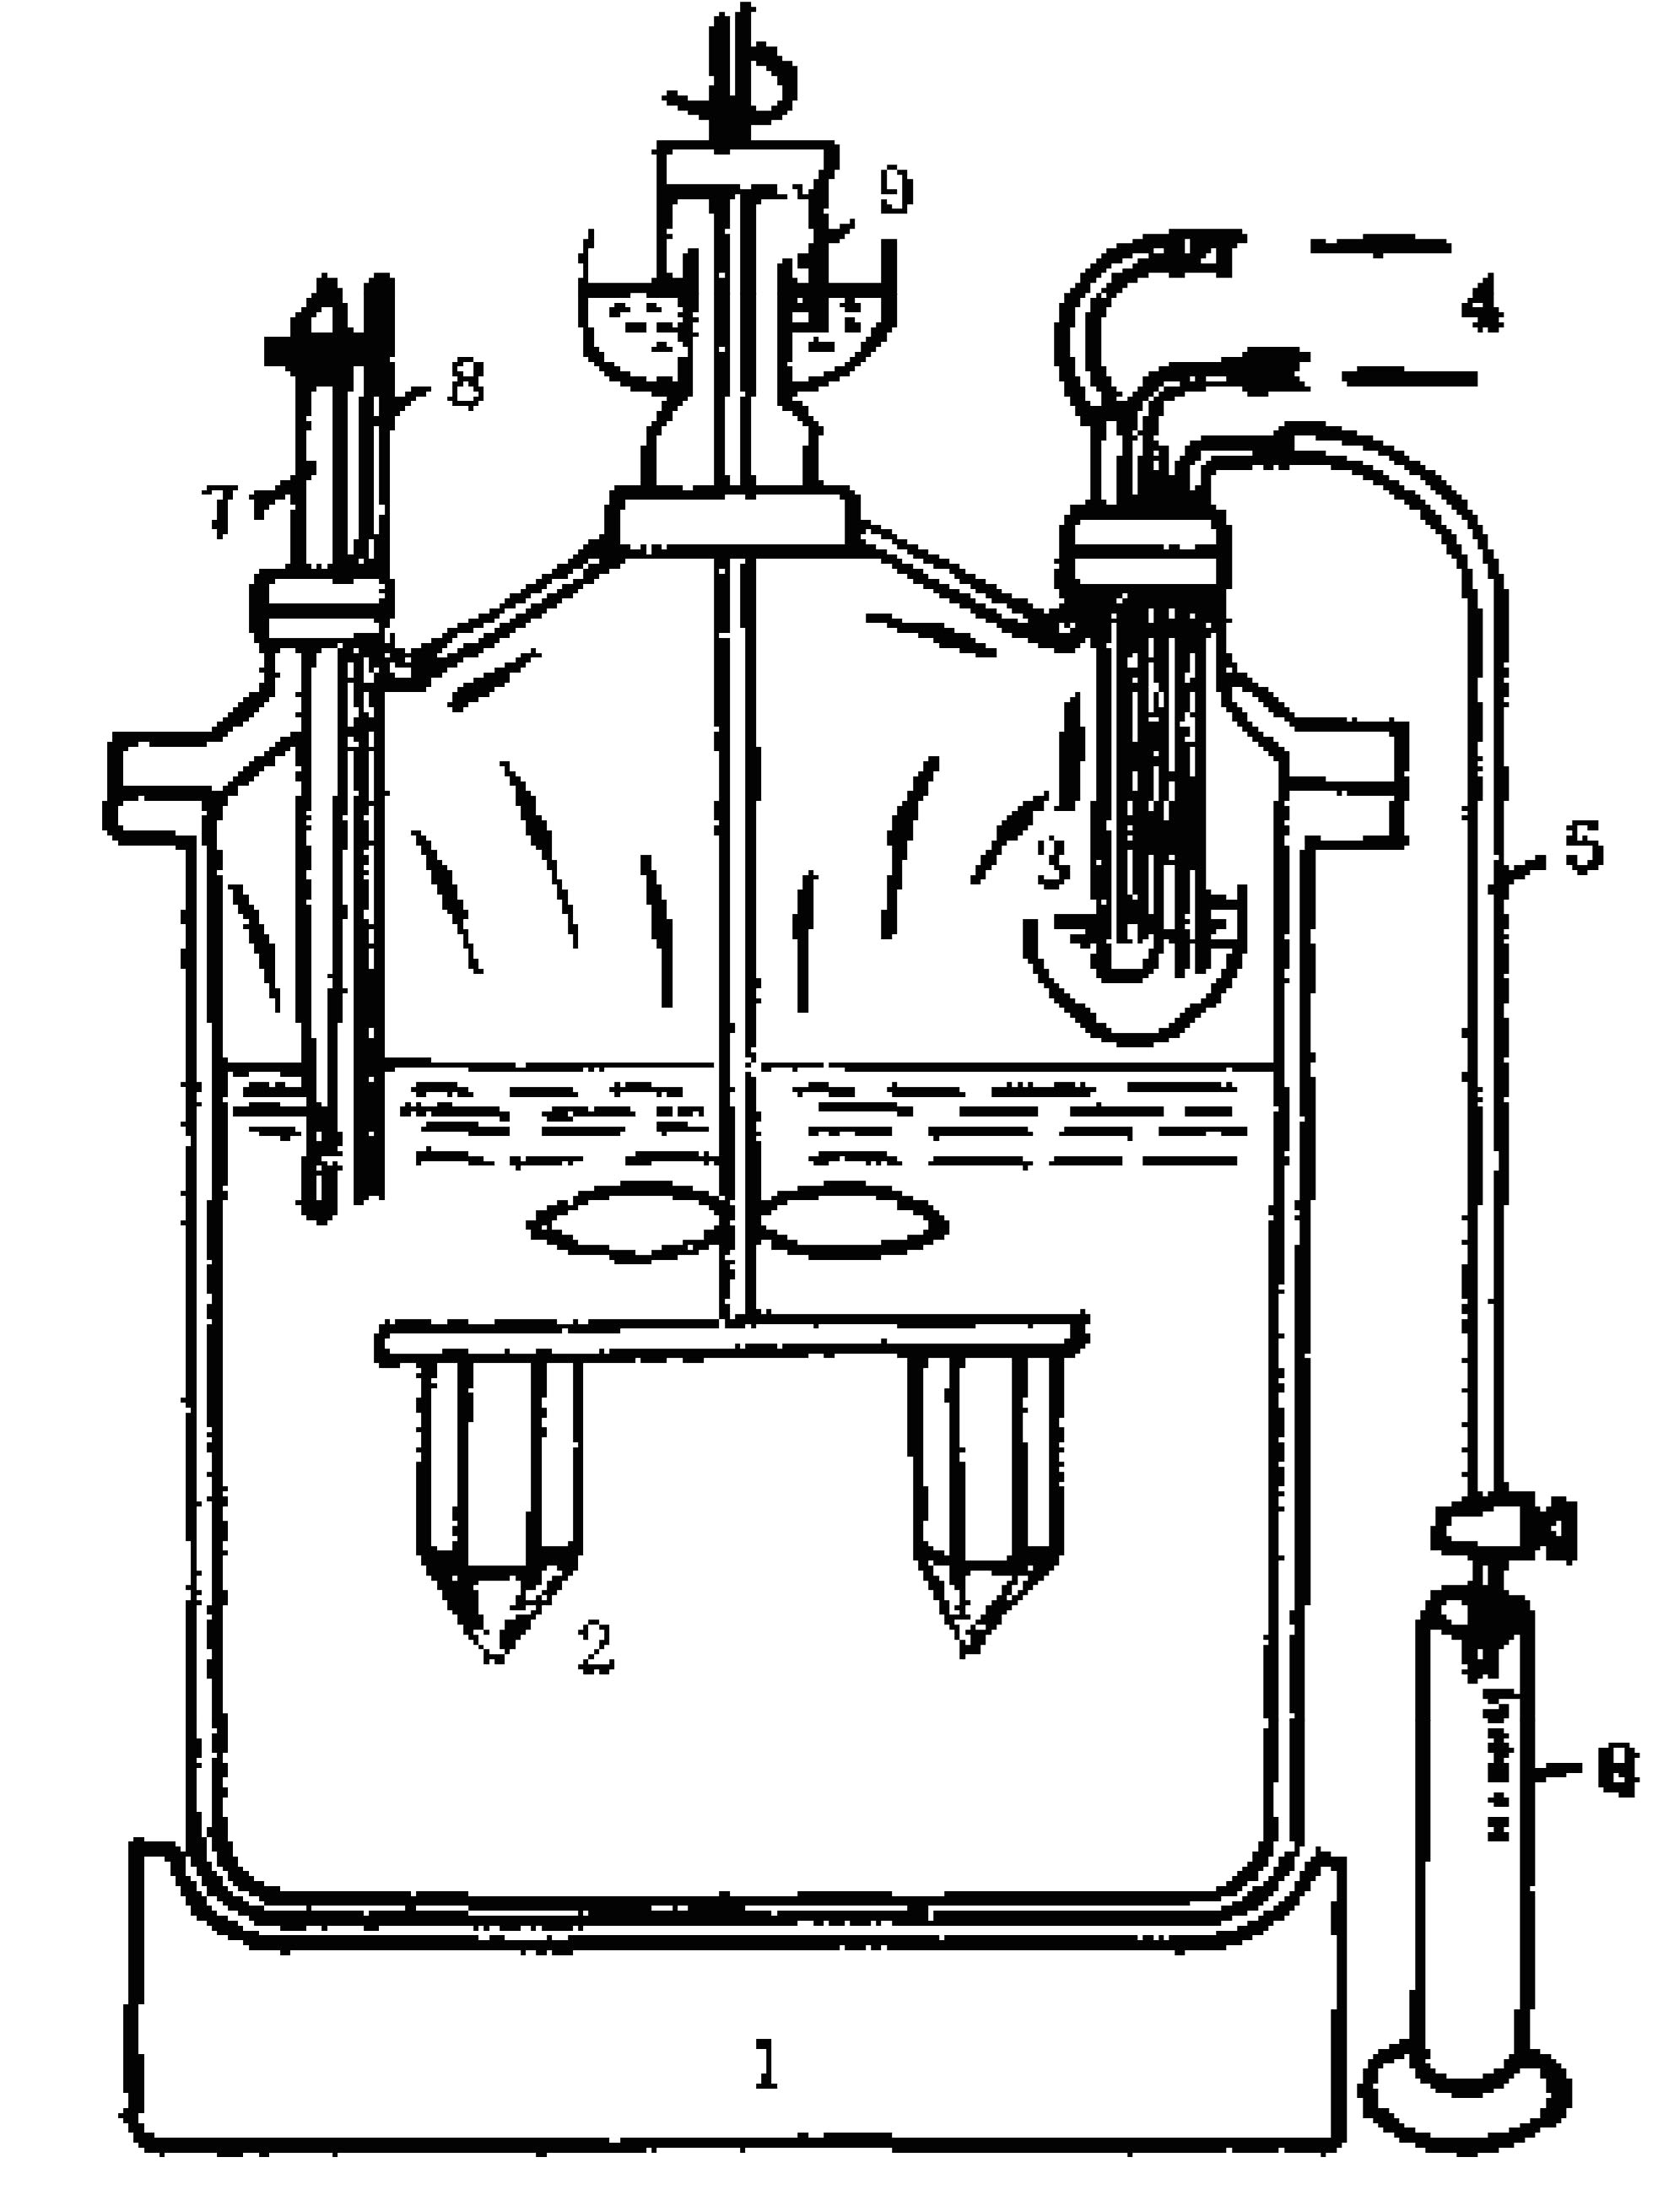
\includegraphics[width=0.4\textwidth]{fig/cp03/img3.23.jpg}
 \caption{蒸发法育晶装置。}
\end{figure}

\begin{figure}[hbt]
 \centering
 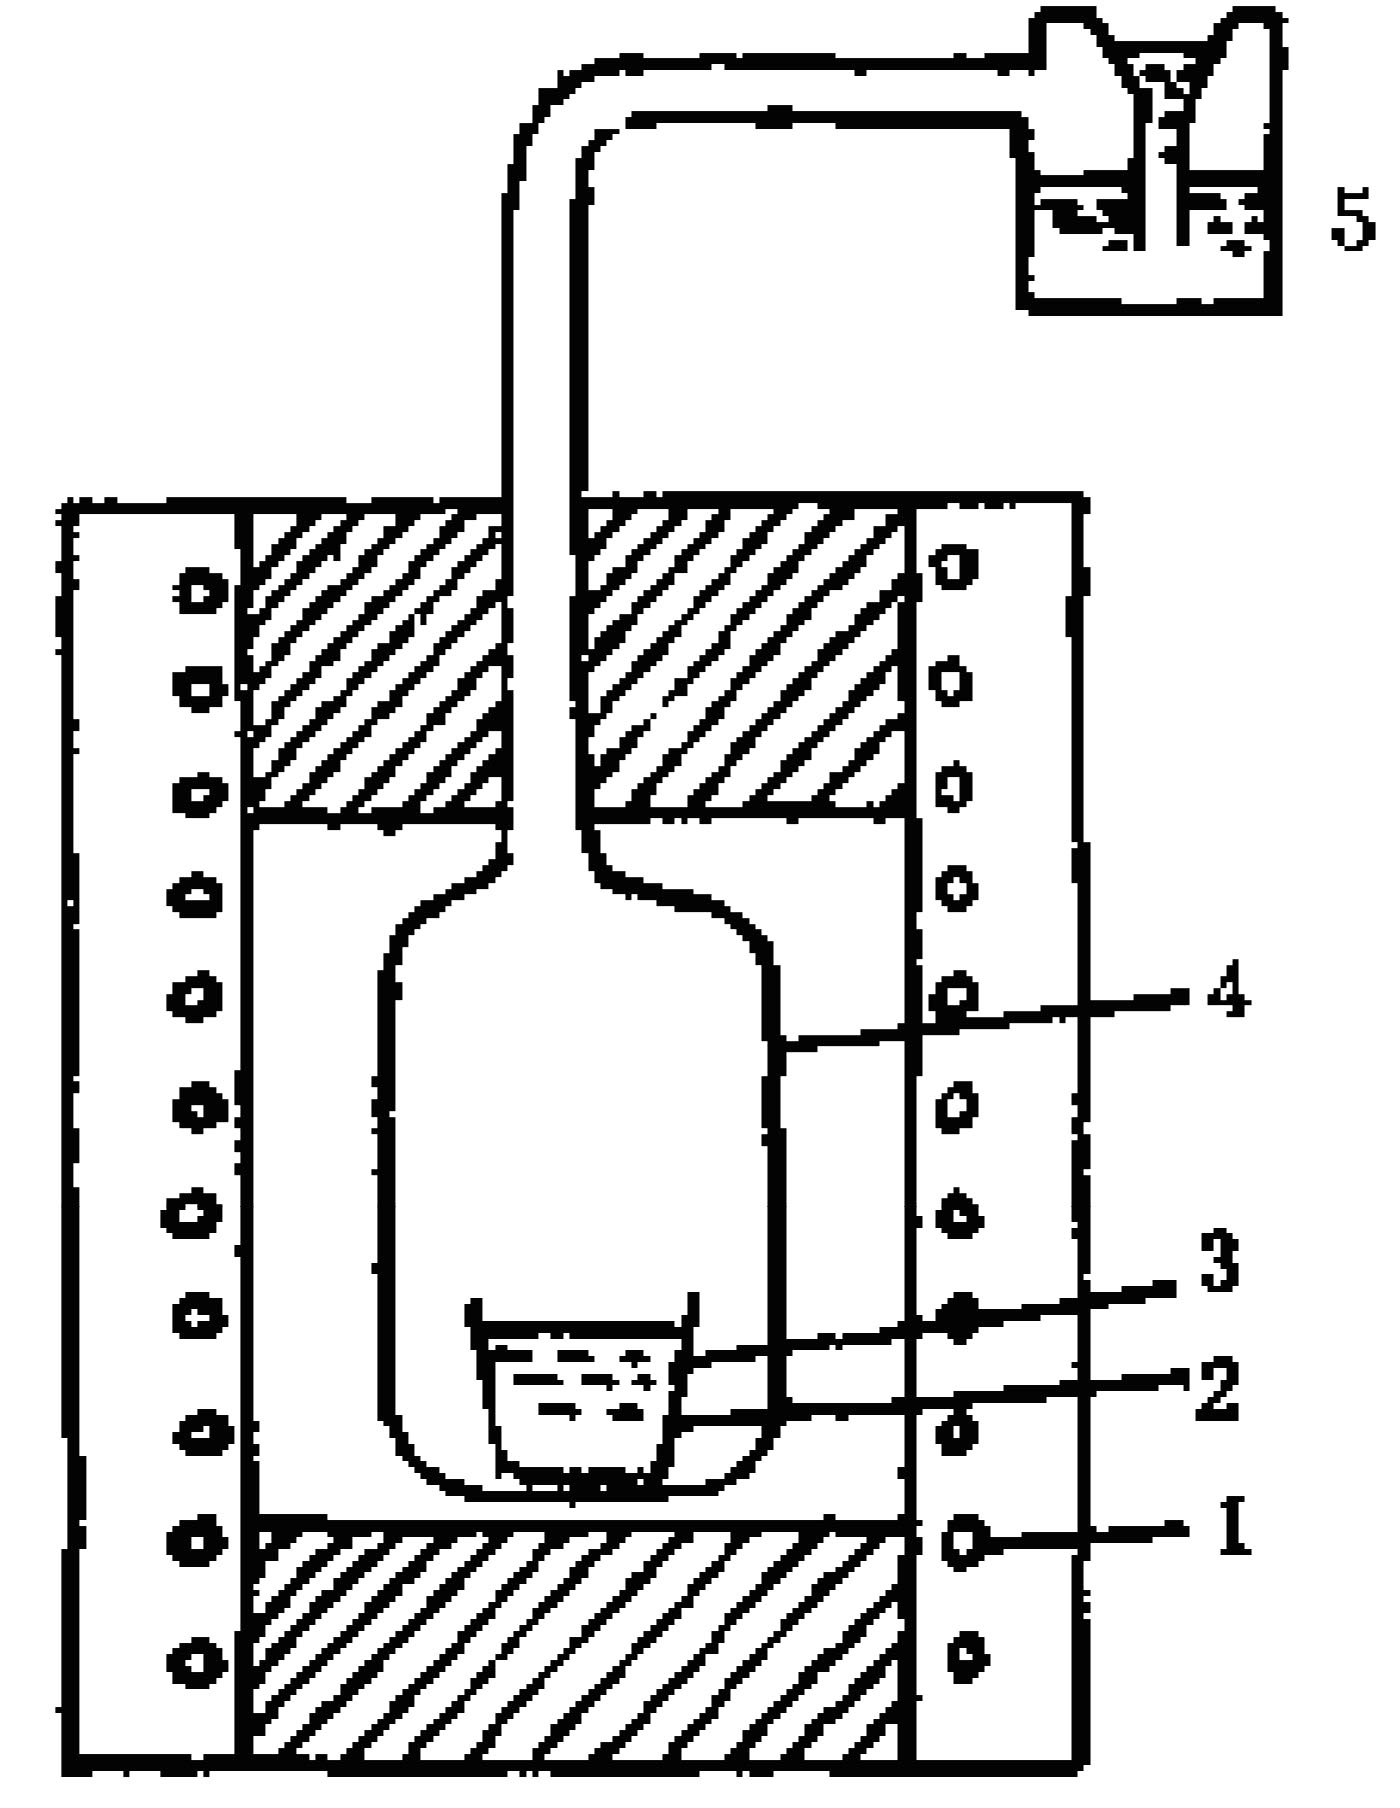
\includegraphics[width=0.4\textwidth]{fig/cp03/img3.24.jpg}
 \caption{生长NdPP晶体的装置。}
\end{figure}

有时体系中某一成分(如水)的蒸发并不是作为溶剂蒸发直接导致晶体生长,而是引起化学反应,间接导致晶体生长,例如在$\rm Nd_2O_3-H_3PO_4$(或$\rm Nd_2O_3-P_2O_5-H_2O$)体系中生长五磷酸钕($\rm NdP_5O_{14}$简称NdPP)晶体,其形成机制可能是
$$ \rm 14\ H_3PO_4 + Nd_2O_3 \xrightarrow{>260℃} 2\ NdP_5O_{14}+2\ H_4P_2O_7+17\ H_2O\uparrow$$

NdPP在焦磷酸($\rm H_4P_2O_7$)中有较大的溶解度,所以不会从溶液中析出,当温度升至300℃以上,焦磷酸逐渐脱水,形成多聚偏磷酸,NdPP在其中溶解度很小,在升温和蒸发过程中,由于焦磷酸浓度降低而使NdPP在溶液中到达过饱和而结晶出来
$$\rm n\ H_4P_2O_7 + NdP_5O_{14} \xrightarrow{>300℃} 2\ (HPO_3)_n + NdP_5O_{14}\downarrow + n\ H_2O\uparrow $$

据此机理,采用图3.24所示装置,在一定的温度下,控制水的蒸发速率就可以生长出质量较好的NdPP晶体。

这种晶体生长方式实际上是晶体在无机溶剂(焦磷酸)的溶液中,通过焦磷酸脱水蒸发而产生缩聚反应,使溶剂不断减少,并使溶质(NdPP)从其饱和溶液中结晶出来的过程。因此将其归入蒸发法。 %蒸发法
\subsection{电解溶剂法}
电解溶剂法是从溶液中生长晶体的一种独特的方法。其原理基于用电解法分解溶剂,以除去溶剂,使溶液处于过饱和状态。显然这种方法只能应用于溶剂可以被电解而其产物很容易自溶液中移去(如气体)的体系。同时还要求所培养的晶体在溶液中能导电而又不被电解。因此,这种方法特别适用于一些稳定的离子晶体的水溶液体系。

电解溶剂法的一半装置如图3.25所示。育晶器中装有铂电极,也起电解槽的作用,当通以稳定的直流电,溶剂就被电解,其速度由电流密度控制。溶液要搅拌以免产生浓差极化。溶液表面用流动液层(如邻二甲苯)覆盖以防溶剂蒸发,电解的产物从冷凝器中排除,在生长过程中,溶液pH应保持稳定。

\begin{figure}[h]
 \centering
 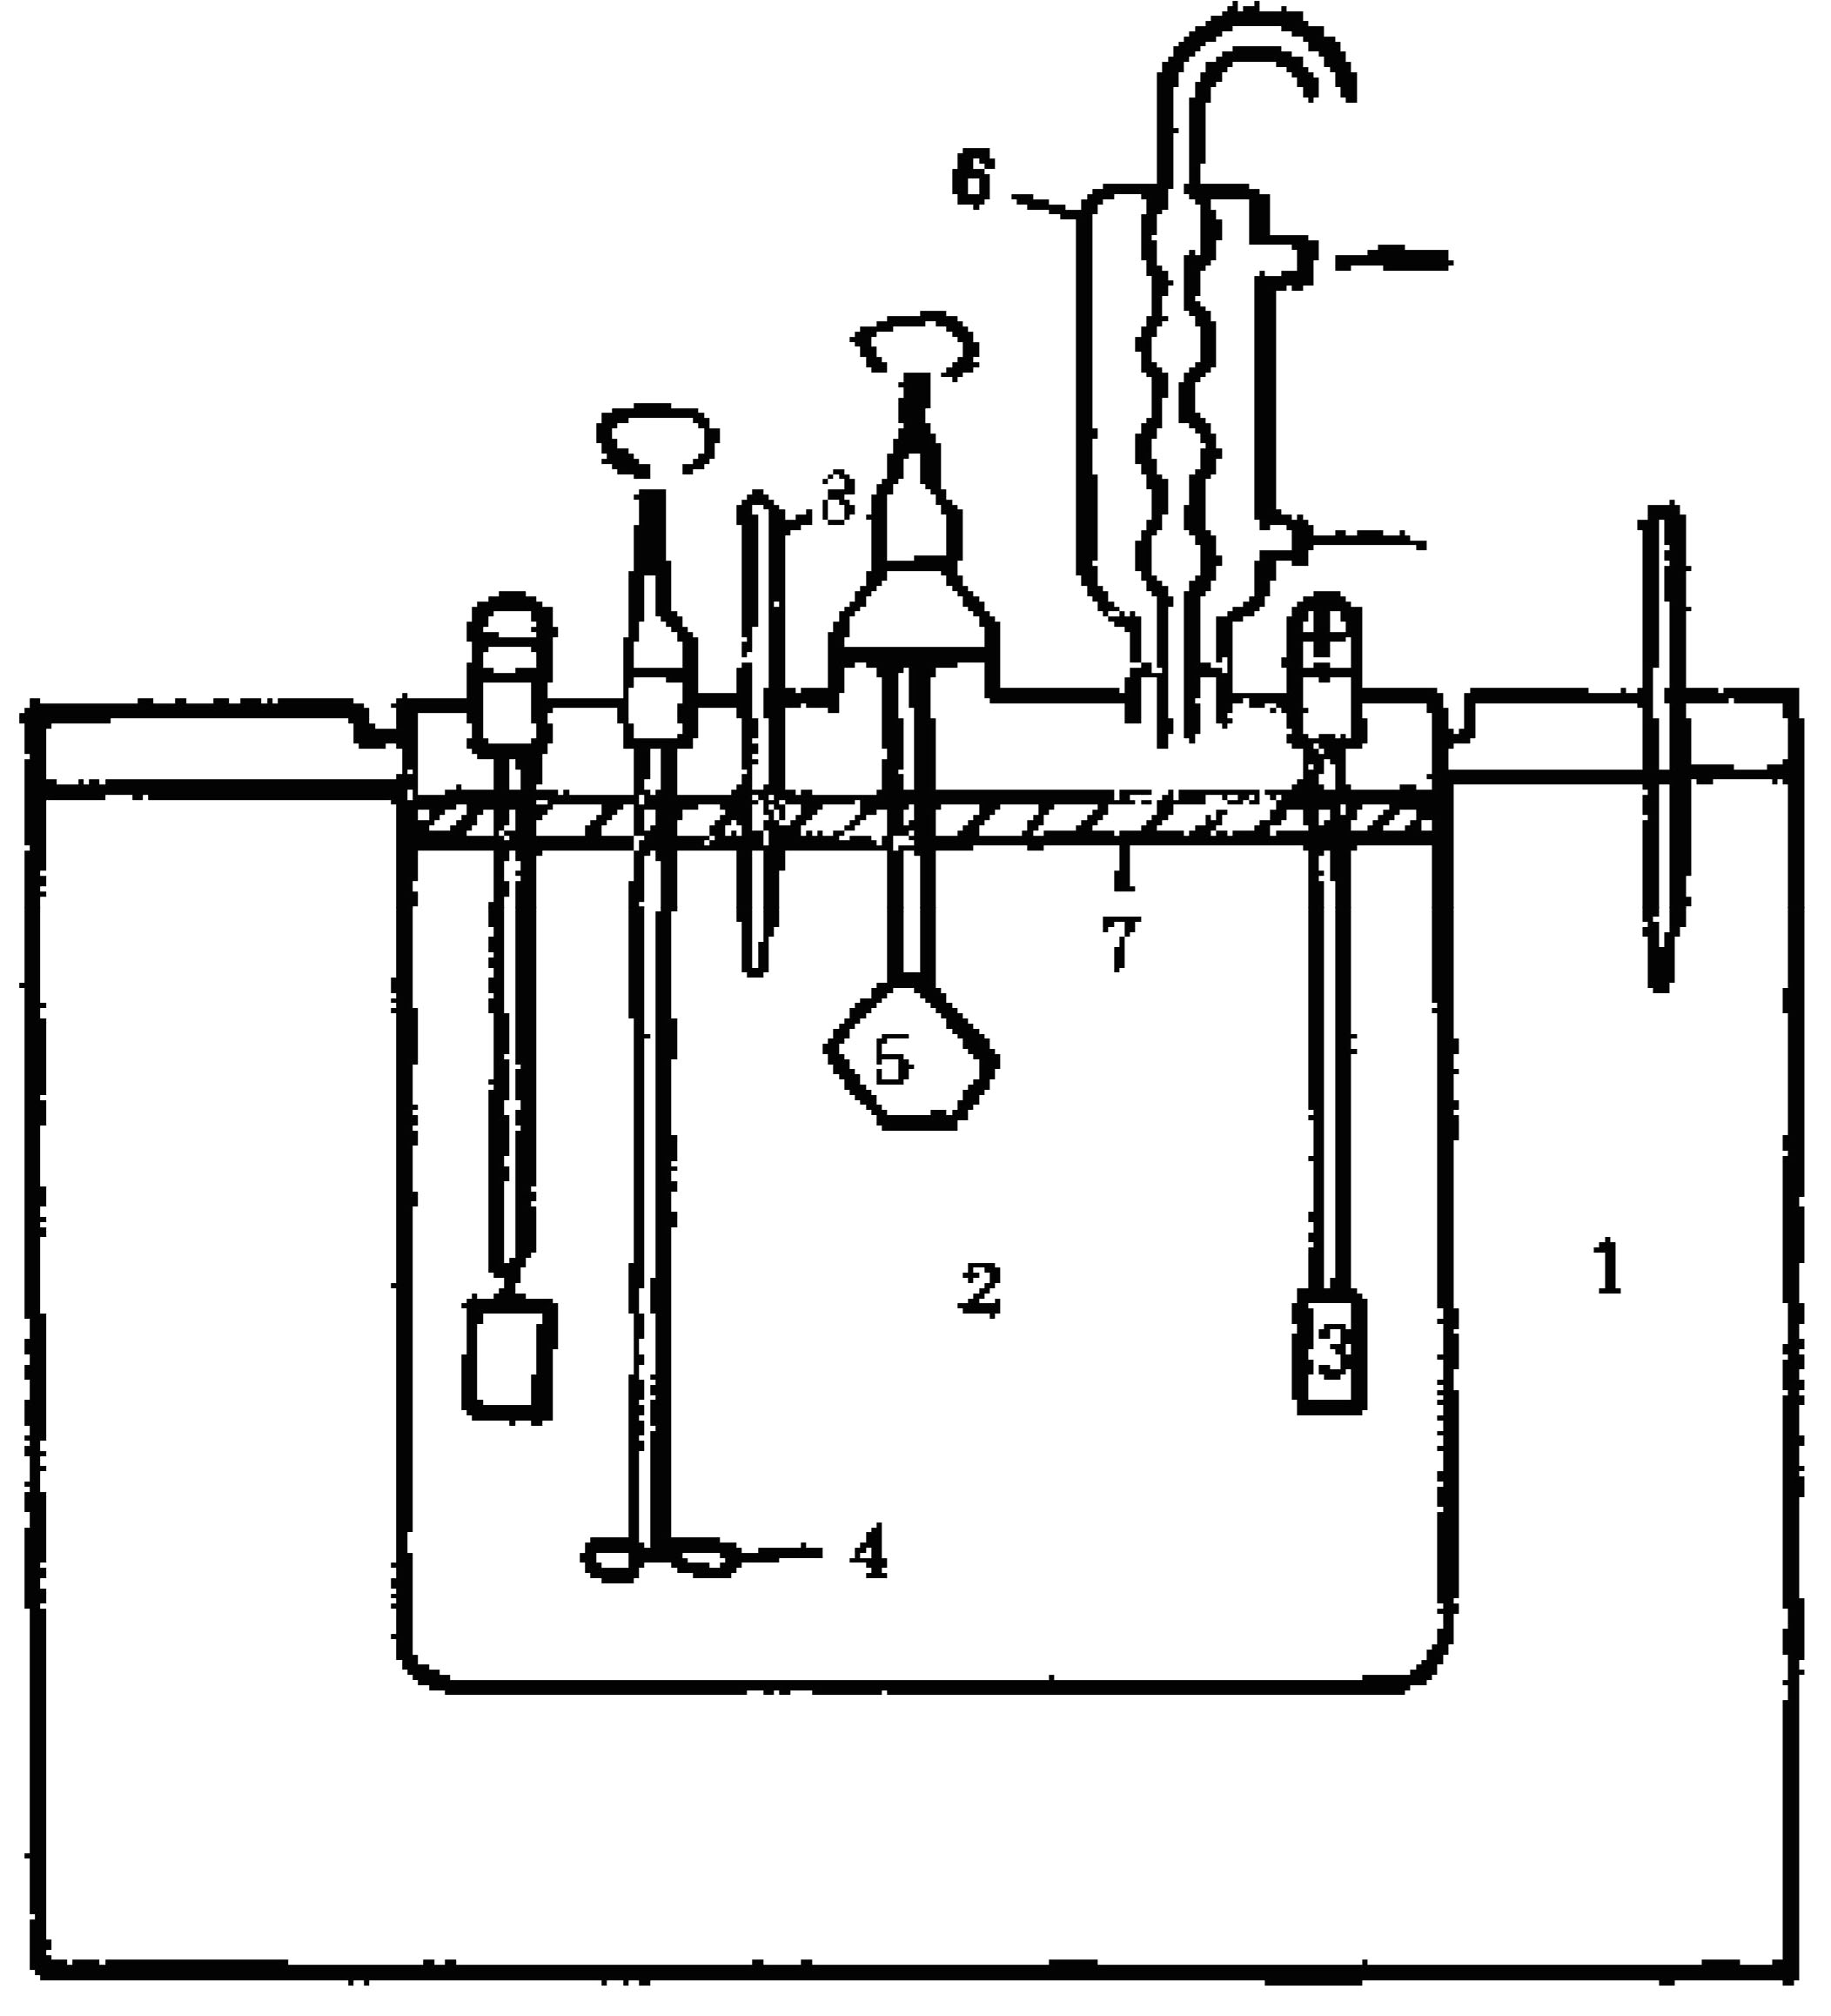
\includegraphics[width=0.5\textwidth]{fig/cp03/img3.25.jpg}
 \caption{电解溶剂法生长晶体装置图。}
\end{figure}

和流动法和蒸发法一样,用电解溶剂法生长晶体也是恒温下进行的。由于过饱和度使用直流电准确控制的,因此和生长温度关系不大,也可在室温下进行(这一点比蒸发法优越,因为温度较低时,蒸发量小,难以控制),也不需要知道溶解度曲线的情况。所以这种方法既适用于溶解度温度系数比较小的晶体,也适用于生长有数种晶相存在,而每种晶相仅在一定温度范围内才能稳定存在的晶体。

用电解溶剂法来生长KDP型(特别是DKDP晶体)获得了满意的结果。因为溶液中存在的常导致这些晶体柱面楔化的一些金属杂质离子(如Fe$^{3+}$,Al$^{3+}$,Cr$^{3+}$等)可以在电解过程中除去,从而消除这些杂质的有害影响。对DKDP晶体可以在低于其转变点的温度下生长,以防止单斜相的干扰,由于分解H$_2$O所需的能量比分解D$_2$O的要低,溶液中的H$_2$O在电解过程中比较容易除去。溶液在生长过程中可以保持较高的氘化程度。图3.26示出在普通转晶育晶器(图3.18)基础上改装的电解溶剂法生长这一类晶体的装置。阳极置于育晶器底部,为使电流均匀通过溶液,在溶液上方安置了两个电极,阴极放在喇叭形口的塑料管内,口上用尼龙网覆盖,使在阴极上产生的氢气引入通风良好的空间,防止其重新进入溶液。在阳极上产生的氧气进入育晶器中溶液上方的空间,保持正压,它投注于减少大气中的水汽和溶液中的氘发生交换而降低其含氘量。由于电解交流也会产生热量,因此也可以不使用底部加热器,而是将交流电直接通过电极加热,使用交、直流并用的加热—电解联合控制装置。晶体在溶液中转动以使溶液浓度均匀。由于溶液是强缓冲溶液,所以电解过程中溶液pH变化不大。

\begin{figure}[htbp]
 \centering
 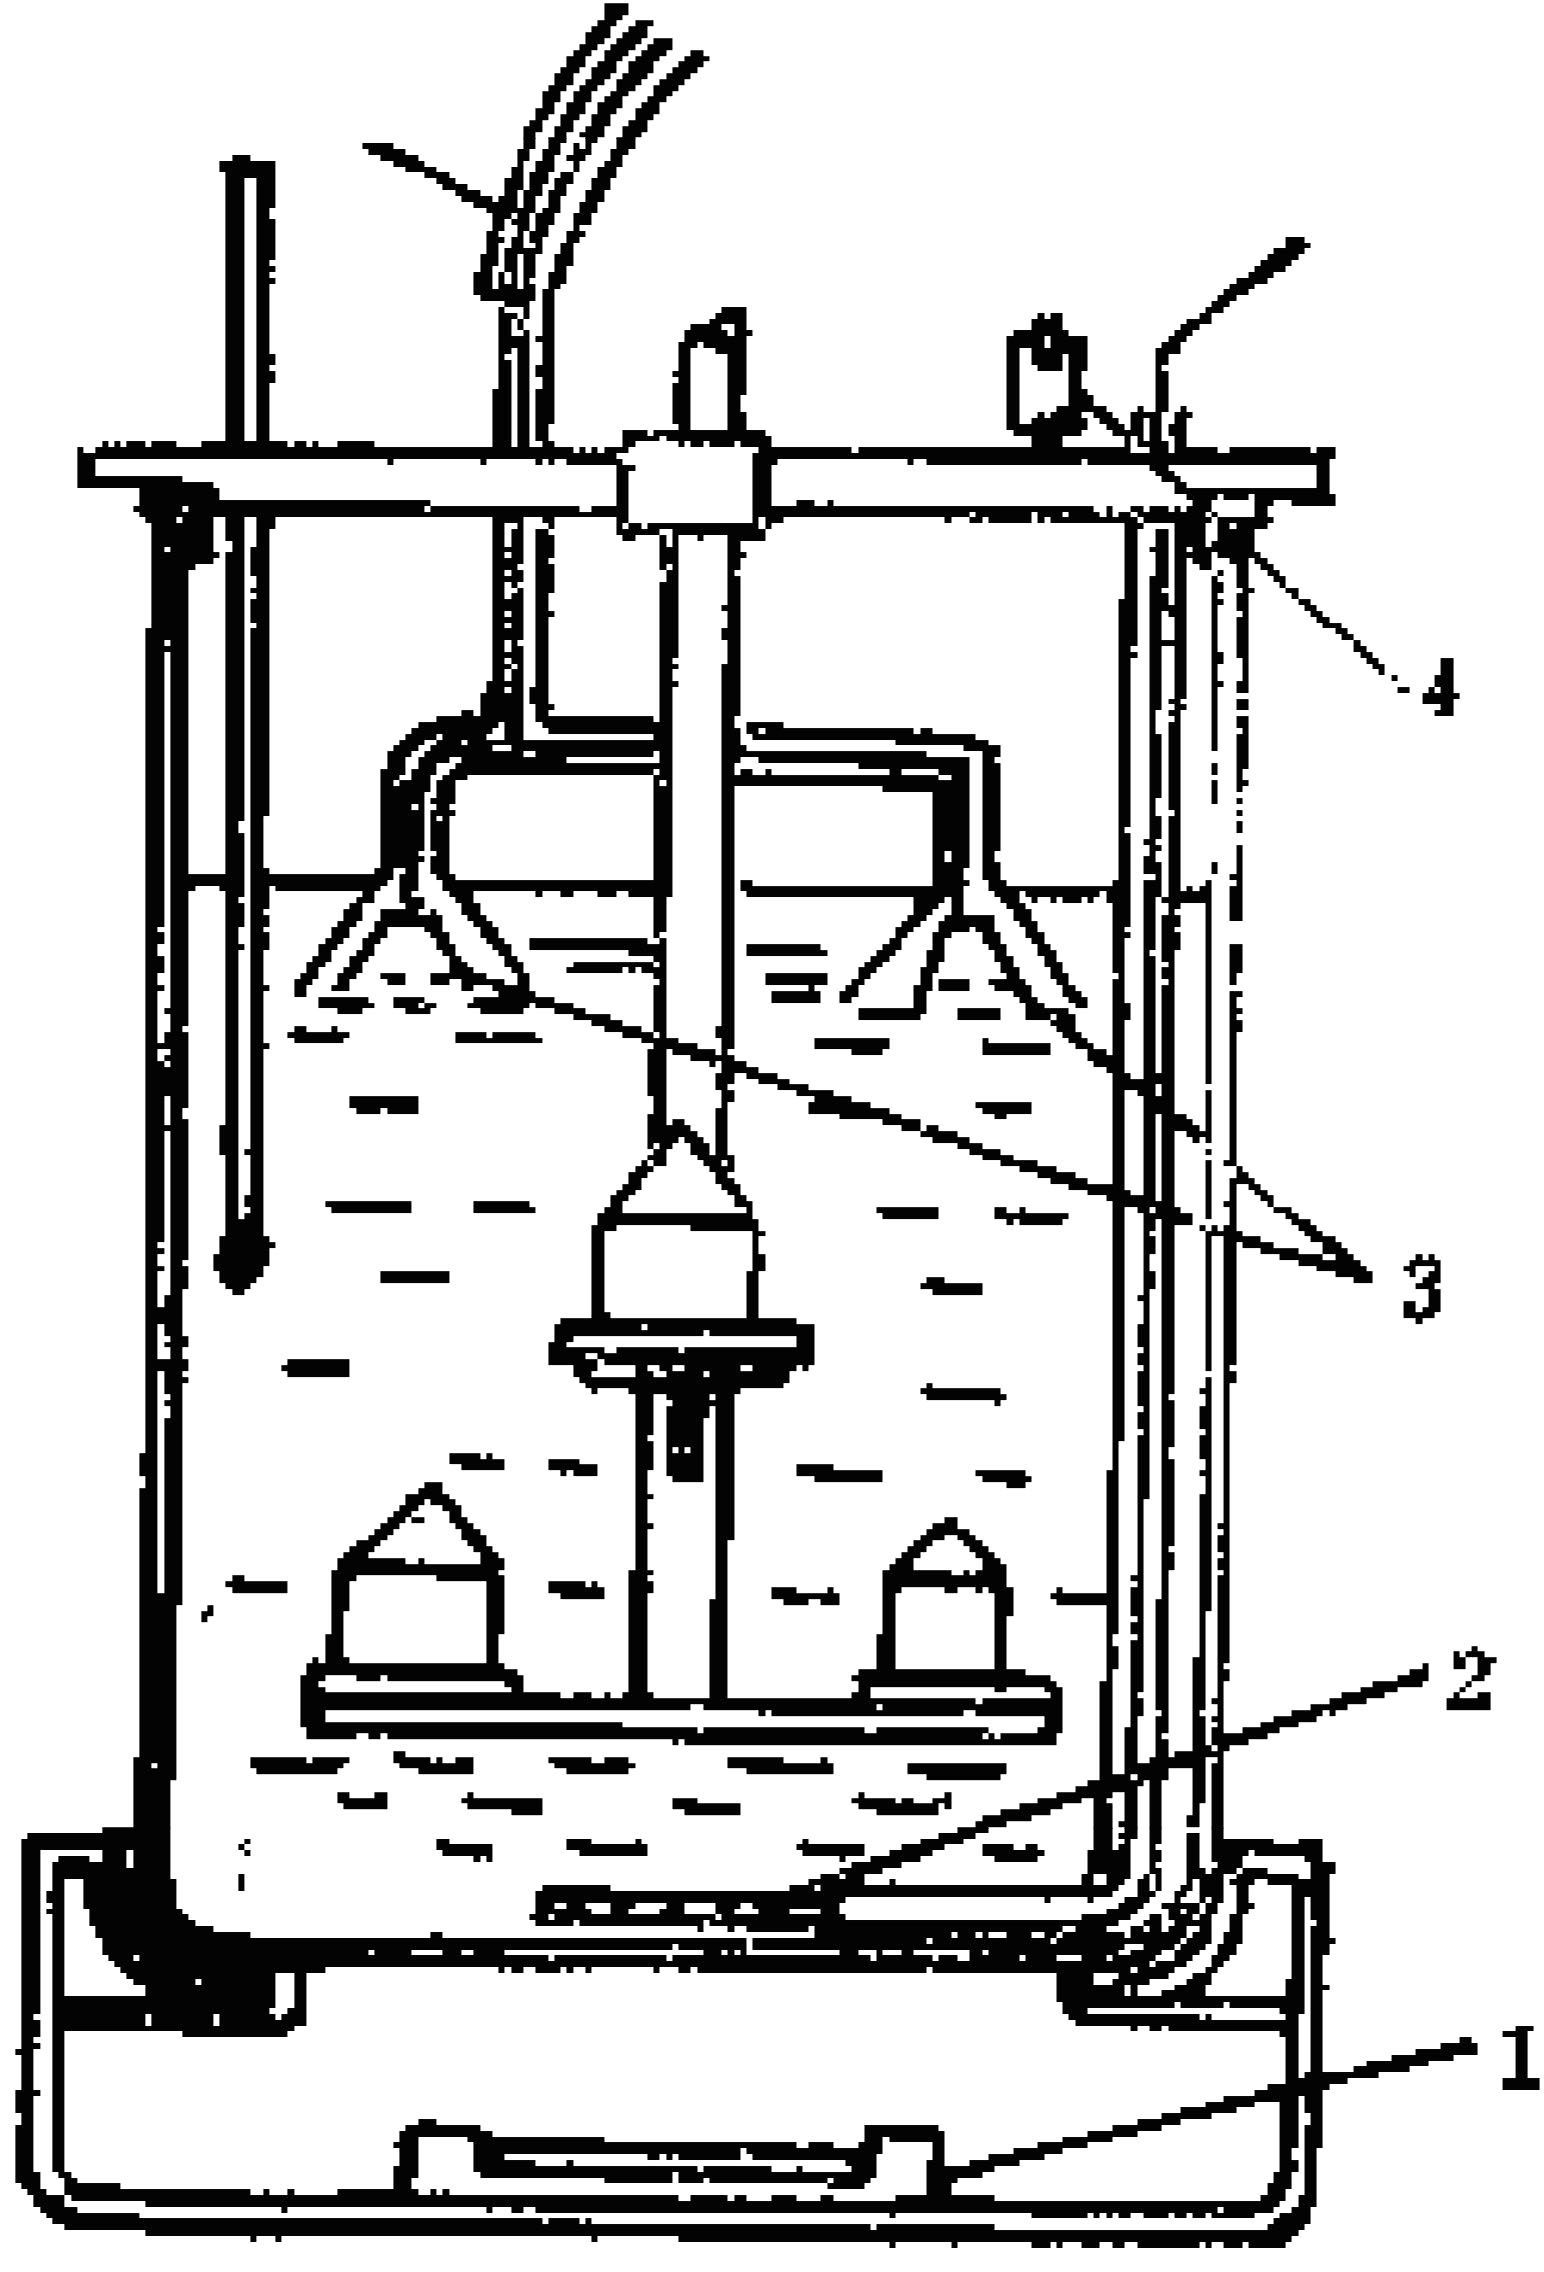
\includegraphics[width=0.4\textwidth]{fig/cp03/img3.26.jpg}
 \caption{由通常转晶育晶器改装的电解溶剂育晶装置。}
\end{figure}

对于从重水溶液中生长高质量的KDP型晶体,电解溶剂法是一种有前途的方法。

除了上述四种从水溶液中生长晶体的方法外,还有凝胶法,有机溶剂法等,这些内容将在下面独立的章节中进行论述。

上述的从溶液中生长晶体的各种方法中,以降温法、蒸发法、流动法最为常用,大部分水溶性晶体都是用这些方法培养的。表3.9列出了从溶液中生长的一些晶体的单晶培养和一般的结晶方法。

(表3.9  从溶液中生长的一些重要晶体)

 %电解溶剂法

\setcounter{section}{3}
\section{溶液中培养单晶生长条件的控制和单晶的完整性}
符合各种技术应用要求的晶体必须具有良好的完整性。溶液法生长晶体的完整性离不开对生长条件的严格控制。在具有良好完整性的前提下,尽量提高晶体的生长速率和利用率是晶体生长工作者始终不渝的追求目标。

\subsection{籽晶}
与有生命的动植物一样,培养优质单晶应选择优良的籽晶。籽晶上的缺陷,如位错、开裂、晶格畸变等在一定的范围内会“遗传”给新生长的晶体。避免使用有宏观缺陷的籽晶,有时还借助于物理光学的方法来挑选籽晶,以减少不利的“遗传”作用。

一般说来,结构和成分与结晶物质相同或相似的晶体取其中任何一部分都可以作为籽晶。但以结构和成分完全相同的完整晶体的一部分作籽晶时为最好。

同位素晶体:DKDP与KDP,DCDA与CDA,DTGS与TGS,DLAP与LAP等由于成分上只存在D与H的差异,结构上差异也不大,故可以互作为籽晶。钾明矾和铬矾的情况也相似。但是籽晶与新生长晶体在结构和成分上的差异会引起晶格失配,在晶体中留下应力,严重时会引起晶体开裂。所以籽晶最好取自相同生长条件下生长出来的完美晶体。

在初次培养一种新晶体时,可先培养出“晶芽”作为籽晶。对于溶解度正温度系数较大的结晶物质,培养“晶芽”是很方便的。先在烧杯中配制适量高于室温5---10摄氏度的饱和溶液,稍过热后注入5---10cm大的培养皿中,用表面皿盖好,让其在室温下冷却结晶,待七八小时后即可将尺寸较大、外形完美的“晶芽”用不锈钢镊子取出,用滤纸吸干溶液即成。如果“晶芽”尺寸不够大,可以把表面皿掀开一条缝,用控制蒸发的方法,让“晶芽”长到需要的尺寸。此法对溶解度温度系数小的结晶物质亦适用。

从已有的大晶体上切取籽晶是最方便和广泛使用的方法。根据晶体生长的习性和日后应用的要求,籽晶可采用“点”状,“杆”状或“片”状等不同的切型。一般来说,切割籽晶时应尽量保留在晶体生长慢的方向上有较大的尺寸。

KTN,$\rm NaNO_3$和NaCl一类晶体,各个方向生长速率相近,故可采用“点”状晶种。使用时将小粒晶种嵌入乳胶管一端,让完整性好的部分露出乳胶管,乳胶管的另一端套到掣晶杆上(图3.27)。“点”状籽晶生长过程恢复区很小,不利的“遗传”因素较易消除,晶体紧包住乳胶管生长,降低了掣晶杆与晶体间的应力。

(图3.27)(图3.28)

TGS和LSH晶体$Z$向生长慢,采用平行于$Z$轴的“杆”状籽晶是合适的(图3.28)。由于在$X$,$Y$方向上生长较快,长出的晶体趋于各向匀称,这就提高了晶体产率和利用率。如采用平行于[111]晶稜的“杆”状籽晶来生产KDP型晶体,生长时恢复区很小,亦不需要成锥过程,对CDA,DCDA这类成锥较困难的晶体特别有意义(图3.29)。

实用上,生长KDP型晶体大都采用$Z$切片籽晶。这类晶体$Z$方向比$X$,$Y$方向生长快很多。$Z$切片籽晶在生长初期有一个恢复自然外形的成锥(俗称“成帽”)过程。生长成帽的地方主要在\{100\}和(001)相交的稜附近。保持籽晶在此稜附近的完整性对成帽质量起关键作用。籽晶片中央部分对生长影响较小,可以作打孔、捆绑或上螺丝将籽晶固定在掣晶架上。平行于KDP\{101\}切片也常用作籽晶,其好处是,平行于自然锥面,晶体生长恢复区小,降低了多个晶面生长引起的生长扇形界,后者使晶体光学均匀性变坏。此外,KDP晶体二类二倍频方向与\{101\{切片的方向接近,可以提高晶体的利用率。

ATGSAS采用平行于(010)的籽晶片,这样可以生长出单畴的大晶片,使整个晶片的均匀性大大提高,更适合于热成像技术上的应用。

晶体的生长习性是受生长条件影响的。所以实际工作中采用什么样的籽晶应同晶体生长习性,生长条件和应用要求结合起来考虑。

(图3.29) %籽晶
\subsection{溶液的处理}

 %溶液的处理
\subsection{介质对晶体生长的影响}
% OCR Product
% To be fixed
实际晶体都是在一定的介质环境中生长的,因此介质必然对晶体(外形和完整性)发生影响,开展这方面的研究,不仅对于培养优质单晶,而且对于探讨实际晶体的形成问题都具有重要的意义,介质对从溶液中生长晶体的影响主要包括以下几个因素:杂质、溶液中氢离子浓度(pH值)、温度、过饱和度和介质运动等。

\paragraph{(1)杂质}通常把与结晶物质无关的少量外来物质称为杂质。杂质在结晶过程中一般是难以避免的。广义的杂质还应该包括溶剂本身,从这个意义上来说,杂质是不能消除的(其含量有时甚至是很大的),因为它本身就是外介质。

杂质对晶体生长的影响是多方面的,研究杂质效应不仅有助于控制结晶过程和单晶的性质,而且在晶体生长理论研究上也有重要的作用,因为杂质影响的机制常与晶体生长动力学的研究紧密联系在一起的。

杂质可以影响溶解度和溶液的性质,例如在生长某些晶体时,常在溶剂中加入一定量(百分之几)的辅助剂或使用混合溶剂,以改变溶解度或溶液的粘度,使有利于晶体的生长(表3.10)。

(表3.10)

杂质也会显著地改变晶体的结晶习性(晶癖),Buckley曾用许多篇幅对此作了专门叙述,在工业结晶中也常应用杂质这一效应,表3.11列出了其中的一些典型例子。

(表3.11)

杂质对晶体质量也有明显的影响。在多数情况下,杂质使晶体的完整性降低,性能变坏,但也存在一些少量杂质离子能改善晶体生长质量,其侧子见表3.12。有时为了改善晶体某一方面的性能,还需加入一些杂质(掺质)。例如在TGS晶体中掺入$\alpha$丙氨酸以防止退极化。

(表3.12)

杂质影响晶体生长有以下三种方式:
\begin{enumerate}[(i)]\itemsep -0.5ex
\item 进入晶体;
\item 选样性吸附在一定的晶面上;
\item 改变晶面对介质的表面能,
\end{enumerate}

杂质进入晶体的机制井不十分清楚,一般来说,由于结晶作用的专一性,生长中的晶体对外来杂质有排斥作用。但有时晶体表面也可以键合杂质质点,特别是它与组成晶体的质点在晶体构造中较为相似时,比较容易均匀地进人晶体,相似性愈大,进入晶体就愈容易,例如在生长DKDP晶体时,H就可以进入D的位置,形成均匀的$\rm K(D_xH_{1-x})_2PO_4$混晶。在掺$\alpha$丙氨酸的TGS晶体(称ATGS)中,$\alpha$丙氨酸之所以能进入TGS晶格中,主要是由于$\alpha$丙氨酸分子(!!!)和甘氨酸分子(!!!)在结构上的相似性。杂质的这种均匀进入通常会对晶体的性质发生影响。当然,这种进入一般是有一定限度的,超过这一限度常会引起晶体构造的不稳定。有时杂质(包括溶剂)也会不均匀地进入晶体,造成包裹物,这主要是由外因引起,如过饱和度过大,溶液搅拌不均匀等。

由于晶体的各向异性,杂质在晶体的不同晶面上经常发生选择性吸附。这种吸附常使某些晶面的生长受到阻碍,因而改变了各晶面的相对生长速度。在杂质改变晶癖的例子中有不少是由这种原因造成的。选择性吸附还普遍具有饱和性,即当溶液中杂质含量超过一定浓度后,它对生长的遏制作用不再随杂质浓度的增大而增长。选择性吸附对晶体的影响方式以进入晶体为主。如在含有$\rm CuCO_3$的溶液中生长KTN晶体时,$\rm Cu^{2+}$只吸附在\{001\}晶面上,阻碍其生长,但对[001]晶带上的晶面却无影响,结果使KTN晶体$Z$向变短,甚至呈板状。\{001\}表层呈深蓝色,说明$\rm Cu^{2+}$已进入了<001>的生长锥。

必须指出,同一种晶面对不同杂质离子或同一种离子对不同晶面选择性吸附影响的程度是很不相同的。例如三价金属离子$\rm Cr^{3+}$,$\rm Fe^{3+}$,$\rm Al^{3+}$很容易在KDP型晶体的柱面上发生选择性吸附,使柱面楔化(图3.37),但其楔化能力却不一样,在相同的杂质浓度下,按$\rm Cr^{3+}>Fe^{3+}>Al^{3+}$递降。这可能与相应水合离子$\rm M(H_2O)_6^{3+}$的稳定性有关,因其稳定性递减次序恰好是$\rm Cr(H_2O)_6^{3+}>Fe(H_2O)_6^{3+}>Al(H_2O)_6^{3+}$。微量的$\rm Cr^{3+}$很容易进入晶体柱面的生长扇形,使此部分呈绿色[图3.37(c)]。

三价金属离子在KDP型晶体柱面上发生选择性吸附,常常使晶体柱面楔化,光学均匀性降低,这固然是其有害的一面,但也有其可利用的一面。在培养大块晶体时,人们按预定的要求 用规定尺寸横截面的种子,不希望横截面再扩大,而在纯度较高的溶液中生长此类晶体横截面会扩大,有时甚至达到无法控制的程度,使光轴方向生长达不到要求的尺寸,为此必须抑制晶体柱面生长,加入一定量有选择性吸附能力的三价金属离子可以实现上述目标。有趣的是,加入三价金属离子后,溶液的准稳区扩大,稳定性大大提高,而柱面上产生的楔化度可通过加大过饱和度得到补偿(图3.31),使KDP型晶体在$Z$向上的生长速度大大提高。

(图3.31)

杂质改变了晶面对介质的表面能,从晶体生长的分子动力学理论来看,这可以看成时改变各种生长过程的能量。如果杂质不进入晶体,只是在溶液中和溶质相互作用,那么只能均匀地改变所有质点的结合能,表现为杂质对溶解度和晶体生长速度的影响。如果杂质进入晶体,则晶格场受到局部破坏。杂质在不同晶面上进入的情况是不一样的,对各个晶面上质点结合能影响的程度也是不相同的,其结果就是改变了各晶面的相对生长速度。

综上所述,杂质的影响包括晶体学、动力学和热力学等方面的效应,影响的主要方式是进入晶体。


\paragraph{(2)氢离子浓度(pH)}在水溶液中存在着大量的$\rm H^+$和$\rm OH^-$,溶液中的氢离子浓度对晶体生长的影响是很显著的。例如提高溶液的pH值会促使KDP型晶体柱面扩展,降低pH值使得LSH和TGS晶体发育较为匀称。如果溶液pH值不合适,即便是其它生长条件合适,也长不出所需尺寸的好晶体。pH影响也是相当复杂的,一般可归纳为以下几种方式:
\begin{enumerate}[(i)]\itemsep -0.5ex
\item pH影响溶解度,使溶液中离子平衡发生变化。
\item pH改变杂质的活性,即改变杂质络合或水合状态,使杂质敏化或钝化。pH的作用也可能改变晶面的吸附能力,因pH对后者有较大的影响。
\item pH直接影响晶体生长,通过改变各晶面的相对生长速度,引起晶体生长习性的变化。例如25摄氏度时,在$\rm pH=3.8$的溶液中,ADP晶体在$X$方向上生长速度为0,晶体沿$Z$方向伸长。当$\rm pH=5.2$时,沿$Z$向生长速度增长不多,但$X$向生长速度却有明显的增加,晶体长成较短的棱柱体(图3.32)。Mullin把$\rm H^+$也看成和$\rm M^{3+}$一样的杂质离子来解释pH的影响机制:溶液中$\rm H^+$以水合离子$\rm H_3(H_2O)_3^+$存在,它在ADP柱面附近表现出稀释效应,阻碍溶质向晶面上扩散,因而遏制了该面生长。当pH升高时,氢离子浓度减小,阻碍作用减弱,柱面生长速度就增加了。
\end{enumerate}


\paragraph{(3)温度}生长温度对晶体的习性和质量都有影响。图3.33示出过饱和度相同、但生长温度不同的$\rm MgSO_4\cdot 7H_2O$晶体的习性变化。因此,可以利用晶体生长习性随温度的变化,选择合适的生长温度以获得所需要的晶癖。

温度本身的影响可以认为是改变晶体生长各个过程的激活能。晶体生长过程很少是纯表面反应或是扩散过程。一般在较低温度下,结晶过程主要由表面反应这一步控制。当温度升高时,生长速度加快,扩散就逐渐成为控制结晶过程的主要步骤了。在较高的温度下生长的晶体,由于结晶质点排斥外来杂质能力的增强,其长出的晶体质量一般要比在较低温度下生长的好些。

(图3.32)
(图3.33)

如果从结晶质点和介质的相互作用这一观点来研究实际晶体的形成过程时,可以把温度的影响看成是溶剂浓度的变化的影响(如果把溶剂看成杂质,也可以归结于杂质变化的影响)


\paragraph{(4)过饱和度和介质运动}过饱和度是结晶的驱动力,由于不同过饱和度会产生不同的生长机制,过饱和度对晶体生长速度、质量和晶体外形影响都很大。晶体在低过饱和度下生长时,速度较慢,晶面发展比较充分,一些高指数的次要晶面容易出露,ADP、KDP等晶体在过饱和度很低时,也会出现类似于杂质离子所造成的柱面楔化现象(图3.37),随着过饱和度的增加,楔化逐渐减轻到最后消失,经过这样的过程生长的晶体并不产生母液包藏。这种在很低过饱和度下出现的生长现象,可能是由于结晶驱动力过小、扩散到柱面附近的溶质质点无力穿过柱面-锥面交界处的“水分子壁垒”所造成的。用放射自显影术研究铁离子在KDP晶体中的分配的实验结果也表明,适当增加过饱和度(在较小的过饱和度范围内)有助于减少铁离子在柱面上的进入。

控制过饱和度是控制溶液晶体生长速度和质量的关键措施。大的过饱和度有利于晶体的自提纯作用和晶形简化,使晶体光学均匀性变好,而生长速度又快。但大的饱和度容易造成晶面上各部分过饱和度差变大,特别是大晶面,容易出现由于生长速度上的差异造成母液包藏。按照理想完整晶体生长模型,在晶面上晶体生长是一层一层依次推送的,在通过台阶扩展堆砌好一层后再开始新层的生长。晶面上过饱和度的差别破坏了这种生长的顺序性。在质点完成一次排列之前,晶面上过饱和度大的区域(图3.34中的$A, B, C$)又开始了新层的生长,晶体构造的完整性遭到破坏,使外面的介质很易进入晶体。所以晶面上过饱和度的差别是为杂质(广义)进入晶体开路的主要外界因素。

(图3.34)

介质的运动对晶体生长速度和完整性都有显著的作用,这种作用往往又和过饱和度紧密联系在一起。介质运动由自然对流、强迫对流和晶体自身生长引起。对流是质量传输和热量传输的主要形式,它影响晶体生长动力学、杂质俘获、组分均匀性、形态稳定性和成核作用。一般来说,随着对流的增大晶体生长速度也增大,直到以生长动力学机制决定生长速度。在无对流的情况下,过饱和度的分布在晶面中心最低,棱边次之,隅角顶点最高。这种分布在过饱和度增大时更为突出,容易发生界面的不稳定,产生母液包藏。在水溶液晶体快速生长中,要求过饱和度和溶液相对于晶体的流苏都很大,使晶体生长机制进入动力学和扩散同时起作用。晶体正反方向转动可以减弱顺着晶体产生的“尾流”,防止母液包藏。溶液的充分搅拌可使整体溶液浓度和温度分布均匀,这对大晶面的稳定生长和防止大生长体系中的自发成核特别重要。
 %介质对晶体生长的影响
\subsection{水溶液晶体的快速生长}
晶体从溶液中生长也就是从稀薄环境相中生长。大量的溶剂和少量的杂质使结晶物质向晶体上生长受到重重阻碍。所以溶液晶体生长和熔体晶体生长在速度上存在数量级的差别。KDP型(DKP,DKDP和ADP等)晶体快速生长技术的发展改变了这种状况,大大缩小了这种差别。生长KDP晶体采用传统的降温法,$Z$向生长速度约1mm/d,而用快速生长方法则可达1---2mm/h,提高了一个数量级。快速生长方法的实质,可以说是人们充分利用介质对晶体生长影响的知识在实践中取得成功的一个范例。

晶面法向生长速度可用简单的经验公式$R=\beta\sigma^n$表示,$\beta$是生长动力学系数,$\sigma$是过饱和度,$n$是反映生长机制的常数。从公式中可知,要想提高晶体生长速度可以从两个方面入手:一是提高$\beta$值,二是提高$\sigma$值。

根据{\timesnewroman Такиво}等的研究结果,在一定的过饱和度下,提高溶液流速可以改变晶体的生长机制,实现快速生长。

Cooper等用自己设计的潜入式离心泵,把液流速度与晶体长度之比值$u/l$提高到$\rm 50s^{-1}$,在50---80℃的范围内,用$\rm 18\times 21mm$(101)扇形片作籽晶,获得3---6mm/d的生长速度。在$10\times10\rm mm$的扇形片籽晶上,生长无宏观缺陷的晶体,生长速度达到11---23mm/d。

提高$\sigma$是提高晶体生长速度最重要的途径。前面已详细地讲过生长机制与过饱和度的关系。通过改变过饱和度控制晶体生长机制,使晶体生长既有较高的生长速度,又符合使用要求是可能的。

{\timesnewroman Зайцева}等用传统的降温法,点状籽晶和控制液流速度在30cm/s(生长动力学机制),通过增大过饱和度,使KDP晶体$Z$向生长达50mm/d,柱面生长25---30mm/d。

在快速生长方法中遇到最大的问题是如何防止自发成核和保证晶体完美生长。超细过滤(筛孔直径小于$0.2\rm\mu m$),提高过热温度(高于饱和温度5---10℃)和延长过热时间(2---3d)对防止自发成核有重要作用。但更重要的是严格控制过饱和度和生长速度间的相适应关系,提高原料和溶液的纯度,减少杂质阻碍生长和防止过饱和度积累。防止二次成核是另一个要注意的问题。在高速液流中,已存在于溶液中的晶体,相互碰撞或与容器壁摩擦都会发生二次成核。{\timesnewroman чернов}等从大量的实验事实中发现,二次成核还与生长中的晶体发生开裂有关。开裂产生的晶体碎片成为新的晶核。

用快速生长方法生长出来的晶体,其完整性与通常方法生长出来的无很大的差别。但在生长条件控制方面要求更加严格。晶体在高过饱和度下生长,在晶体表面,特别是在大晶面上浓度空间分数不得不均匀性更易发生,对温度波动也更敏感,造成母液包藏的机会更大。在生长机制上,不仅仅是动力学机制,而且对流-扩散机制也同时起作用,晶体生长趋向于粗糙化,细微裂纹常可在KDP晶体的柱面上看到。晶体开始生长阶段的恢复区,在籽晶与新生长晶体间起着晶格匹配的缓冲作用,快速生长把这个区域缩小,使籽晶上的缺陷更易延伸进新生长的晶体中,此时采用点状籽晶是合适的。快速生长的晶体,其下面性质甚至比常规生长的更优越:KDP(100)生长速度增大时,进入(100)生长扇形的杂志浓度降低,而(101)生长扇形中两种方法杂质浓度变化不大。快速生长晶体中不存在常规生长晶体中常见到的生长层和位错束,也不存在其他折射率不均匀的结构,晶面间的生长扇形界消失,表现出有更好的光学均匀性。

综上所述,水溶液晶体快速生长不仅可以大大缩短生长周期,提高生产效率,降低生产成本,而且使晶体某些性能得到改善。尽管快速生长条件苛刻,控制困难,但只要我们更深入地研究介质对晶体生长影响的动力学,更准确地把握生长条件、生长机制和晶体性质之间的关系,实现按预想要求既快又好地培养出特定需要的晶体是完全可能的。 %水溶液晶体的快速生长
\subsection{水溶性晶体常见的宏观缺陷}
 %水溶性晶体常见的宏观缺陷


\section{凝胶法晶体生长}
凝胶法晶体生长的发展史可追溯到1896年,因为在这一年中,Liesegang观察到了微溶盐在动物胶中周期性结晶现象,这种现象被后人称为Liesegang环。随后,Fisher和Simons等提出了“在完全可控制的条件下,几乎所有的物质的晶体生长,凝胶均可成为良好的介质”的论点。1965年Henish发表了酒石酸钙在凝胶中生长的著名论文。1970年,Henish的专著《凝胶法晶体生长》出版,全面论述了凝胶法晶体生长的全貌与发展动向。从此以后,凝胶法生长晶体在国际范围内有了进一步的\footnote{原文作“地”}发展。

\subsection{凝胶法晶体生长特点}
与通常广泛应用的溶液法、熔体法、熔盐法和气相法等相比,凝胶法晶体生长是一种易于被人们忽视的方法,所使用的育晶设备虽然较为简单,但所涉及的物理化学过程变化多样,此方法本身具有下述的一些独特的优点。

\begin{enumerate}[(1)]\itemsep -0.5ex
\item 凝胶质软、性惰、多孔、半透明,且为不流动的半固体,凝胶介质有效地控制了流体的对流、湍流及外界扰动的发生。凝胶保持了化学上的惰性,且无害于晶体生长。凝胶骨架对晶体生长起到了“三维坩埚”支撑作用,它自然地服从于晶体生长形状,防止了晶体与容器底部或器壁的碰撞,使晶体保持完全无损的状态。
\item 凝胶具有微孔结构,有过滤、隔离成核和抑制成核的作用,因此不仅可使晶体降低杂质污染,并且有益于均匀成河以及均匀掺质晶体生长的研究。
\item 由于凝胶法晶体生长过程是在近于室温环境下进行的,故所生长出的晶体含有较少的热缺陷,从而提高了晶体的完整性。
\item 实际上,由于凝胶可以降低化学试剂的扩散速度,因此可以控制溶质的扩散速率和成核速率,有利于进行晶体生长基本理论的研究。
\item 凝胶法所用的育晶装置简便,化学试剂用量较少,生长的晶体品种较多,适用性很广,便于为研制新型功能晶体材料提供测试样品。
\end{enumerate}

事物总是一分为二的,凝胶法虽然有上述优点,但无疑也存有不足之处,如凝胶虽有抑制成核的作用,能减少非均匀成核的概率,但还很难保证在凝胶中仅有少数几个晶核成长,因此在一般情况下,生长线度为厘米级以上的晶体,除针状晶体外,当前还存在着一定的困难。
 %凝胶法晶体生长特点
\subsection{凝胶的制备、性质和结构}
凝胶是一种具有半固态、富液体、高粘滞性且含有微孔的二组分体系,其中一个组分的分子键合成三维网络,而另一组分通过渗透而形成连续相。凝胶介质不仅是指由硅酸钠溶液制备的硅水凝胶,而且还包括各种有机凝胶,例如从海藻中得到的碳水化合物高聚物(琼脂\footnote{原文作“酯”。}胶)、类似于蛋白质结构的明胶、聚丙烯酰胺、醋酸纤维、四甲氧基硅、四乙氧基硅、硬脂酸盐、铝酸盐等。但硅水凝胶是最普遍使用的一种凝胶,这是由于它比其他有机凝胶更适用于绝大多数晶体的生长。

将硅酸钠($\rm Na_2SiO_3\cdot 9H_2O$)加入水中,酸化后可有硅酸产生,硅酸的一个重要特性是它的聚合作用,影响硅酸聚合作用的因素较多,其中最重要的因素是溶液的酸度。胶凝时间与溶液的pH值的关系曲线如图3.40所示。

(图3.40)

欲得某一确定pH值的凝胶介质,在不断搅拌情况下,准确地加入需要量的酸于硅酸钠水溶液中,该溶液的酸度值决定着凝胶的聚合过程和速度。胶凝时间可从几秒钟、几分钟到几天、几十天或更长的时间。

当硅酸钠在强酸溶液中时,硅酸离子的逐步酸化过程为

(化学图)

氢离子与硅酸中的氧原子结合后,硅氧(!!!化学图!!!)键长即增加。若配位在Si原子周围的$\rm Si-O$键键长都增加,则其配位数即可增大。因此至少在$\rm H_3SiO_4^+$离子(式IV)内的Si的配位数可增到6,可写为

(化学图)

在碱性溶液中,硅酸存在的形式为式(I)和式(II),两者均带负电荷,顾客认为不易起聚合作用或聚合作用极慢,且随碱度的增加而聚合减慢。

在微碱性、中性和微酸性溶液中,硅酸存在的主要形式为式(II)和式(III),两者相遇便可发生聚合作用,从而生成

(化学图)

此种聚合将以$\rm Si-O$键为基础在三维空间延续而形成网络结构。

在较高酸度的溶液中,离子(III)与(IV)相互作用,聚合成为

(化学图)

以上两种类型的聚合反应机制,前者有$\rm OH^-$离子释出,故在聚合过程中溶液的pH值增高,而后者会使溶液的pH值略有降低。当两种反应同时进行时,溶液的pH值便无明显的\footnote{原文作“地”。}变化。

采用酒石酸、醋酸或硝酸作为胶凝剂所制得的凝胶均为透明的。但弱酸作为胶凝剂应用的比较多,这首先是由于用弱酸作胶凝剂,凝胶的pH值随时间变化较小;其二是由于无机酸或多或少地对晶体生长具有一定的损害作用。但使用何种酸为宜,则要视所生长晶体的类型而定。

将酸加入硅酸钠溶液中时,须严防凝胶中气泡的形成,若气泡一旦形成,将很难把气泡从凝胶中排除。此乃往往会阻止晶体生长。

凝胶液的pH值是决定凝胶结构及其性质非常重要的因素,同时在晶体生长过程中也起着重要的作用。硅水凝胶的结构网络,具有两种类型的微孔,一类微孔接近分子尺度,另一类表现为正常的毛细管大小。硅水凝胶的X射线衍射花样同硅玻璃相比,凝胶所具有的均匀性差些。在温和的条件下对硅水凝胶进行干燥,凝胶的总体积变化甚小,干燥过的凝胶易于作X射线衍射实验,可获得更多的结构信息,在对比的情况下,对硅水凝胶也可获得很有意义的实验结果。经估算,硅水凝胶的有效微孔直径约为$5-10\rm\ nm$,脱水收缩作用对微孔平均尺寸的影响甚小。此外,在制备凝胶时所采用的酸的性质和浓度,硅酸钠溶液的密度及硅酸钠的纯度,环境温度,化学试剂在凝胶中的浓度等都是影响凝胶法晶体生长的重要因素。

 %凝胶的制备、性质和结构
\subsection{凝胶法晶体生长的类型}

 %凝胶法晶体生长的类型
\subsection{成核及其控制}

 %成核及其控制
\subsection{晶体生长机制}

 %晶体生长机制
\subsection{凝胶法晶体生长的最新进展}

 %凝胶法晶体生长的最新进展



